\documentclass[12pt]{article}
\usepackage{graphicx,psfrag,epsf}
\usepackage{enumerate}
\usepackage{natbib}
\usepackage{amsfonts}
\usepackage{amsmath}
\usepackage{float}
\usepackage{amssymb,mathabx}
\usepackage{algorithm, algpseudocode}
%\usepackage{cite}
\newcommand{\blind}{0}

\addtolength{\oddsidemargin}{-.75in}%
\addtolength{\evensidemargin}{-.75in}%
\addtolength{\textwidth}{1.5in}%
\addtolength{\textheight}{1.3in}%
\addtolength{\topmargin}{-.8in}%

% formatting tweaks
\newcommand{\te}{\!=\!} % thin equals
\newcommand{\tneq}{\!\neq\!}
\newcommand{\naive}{na\"{\i}ve}
\newcommand{\Naive}{Na\"{\i}ve}
\newcommand{\Levy}{L\'{e}vy}
\newcommand{\myvcenter}[1]{\ensuremath{\vcenter{\hbox{#1}}}} % vertical centering

% bold and caligraphic letters
\newcommand{\ba}{\mathbf{a}}
\newcommand{\bb}{\mathbf{b}}
\newcommand{\bc}{\mathbf{c}}
\newcommand{\bd}{\mathbf{d}}
\newcommand{\bg}{\mathbf{g}}
\newcommand{\bh}{\mathbf{h}}
\newcommand{\bs}{\mathbf{s}}
\newcommand{\bu}{\mathbf{u}}
\newcommand{\bw}{\mathbf{w}}
\newcommand{\bx}{\mathbf{x}}
\newcommand{\by}{\mathbf{y}}
\newcommand{\hyp}{{\mathcal H}}
\newcommand{\model}{{\mathcal M}}
\newcommand{\data}{{\mathcal D}}
\newcommand{\Z}{{\mathcal Z}}
\newcommand{\N}{{\mathcal N}}
\newcommand{\M}{{\mathcal M}}
\newcommand{\F}{{\mathcal F}}
\newcommand{\vS}{{\vec{S}}}
\newcommand{\cS}{{\mathcal S}}
\newcommand{\vcS}{{\vec{\mathcal S}}}
\newcommand{\cT}{{\mathcal T}}
\newcommand{\cN}{{\mathcal N}}
\newcommand{\cV}{{\mathcal V}}
\newcommand{\ocS}{\overline{\mathcal S}}
\newcommand{\Tu}{\mathcal{T}^{\cup}}
\newcommand{\Su}{\mathcal{S}^{\cup}}
\newcommand{\vSu}{\vec{\mathcal{S}}^{\cup}}
\newcommand{\Mu}{\mathcal{M}^{\cup}}
\newcommand{\muu}{\mu^{\cup}}
\newcommand{\vmuu}{\vec{\mu}^{\cup}}
\newcommand{\mul}{\mu^{<}}
\newcommand{\tmuu}{\tilde{\mu}^{\cup}}
\newcommand{\oSigma}{\overline{\Sigma}}
\newcommand{\vSigma}{\vec{\Sigma}}
\newcommand{\dif}{\mathrm{d}}

% arrows without lots of space
\newcommand{\la}{\!\leftarrow\!}
\newcommand{\ra}{\!\rightarrow\!}
\newcommand{\lra}{\!\leftrightarrow\!}

\newcommand{\fwd}{\mathtt{f}}
\newcommand{\bck}{\mathtt{b}}

% Miscellaneous mathematics
\newcommand{\nth}{^{\left( n \right)}}
\newcommand{\mth}{^{\left( m \right)}}
\newcommand{\nnth}[1]{^{\left(#1\right)}}
\DeclareMathOperator*{\argmax}{argmax}
\DeclareMathOperator*{\argmin}{argmin}
\newcommand{\pdd}[2]{\frac{\partial #1}{\partial #2}}

% Colors
%\usepackage{color}

\newcommand{\txss}{\textsuperscript}
 \newcommand{\defeq}{\stackrel{\textup{\tiny def}}{=}}

% defined again below
%\def\l({\left(}
%\def\r){\right)}



\DeclareMathOperator*{\KL}{KL}

\def\bS{\mathbf{S}}
\def\tbS{\tilde{\bS}}
\def\tS{\tilde{S}}
\def\ts{\tilde{s}}
\def\tt{\tilde{t}}
\def\tT{\tilde{T}}
\def\tA{\tilde{A}}
\def\tI{\tilde{I}}
\def\tP{\tilde{P}}
\def\tR{\tilde{R}}
\def\tW{\tilde{W}}
\def\tw{\tilde{w}}
\def\tF{\tilde{F}}
\def\tG{\tilde{G}}
\def\tE{\tilde{E}}
\def\bL{\mathbf{L}}
\def\E{E}
%\newcommand{\mW}{{\mathcal W}}
\newcommand{\mW}{{|W^\downarrow}|}
\newcommand{\assign}{\doteq}

\def\ind{1}

\newcommand{\avg}[1]{\langle{#1} \rangle}

\def\naive{na\"{\i}ve}
\def\hlambda{\hat{\lambda}}
\def\ulmb{\underline{\lambda}}
\def\olmb{\overline{\lambda}}
\def\uR{\underline{R}}
\def\oR{\overline{R}}
\def\Reps{R^{\epsilon}}
\def\leps{\lambda^{\epsilon}}

% these break default latex commands for, e.g., Swedish names
%\def\l({\left(} 
%\def\r){\right)}

\def\matern{Mat\'{e}rn }

\newcommand{\NOTE}[1]{\textcolor{red}{[#1]}}
\newcommand{\vinayak}[1]{\textcolor{red}{[Vinayak: #1]}}
\newcommand{\boqian}[1]{\textcolor{blue}{[Boqian: #1]}}
\newcommand{\given}{\,|\,}

\newcommand{\PP}{\text{PoissProc}}
\newcommand{\from}{\text{ from }}
\newcommand{\Mx}[1]{{\max_s |A_s(#1)|}}
\newcommand{\mx}[1]{{\min_s |A_s(#1)|}}

\newcommand{\SM}{B}
\newcommand\numberthis{\addtocounter{equation}{1}\tag{\theequation}}

\newcommand{\lb}{\ell}
\newcommand{\ub}{u}
\newcommand{\algname}{Rao-Teh}
\def\ctheta{\theta}
\def\ntheta{\theta'}
%\def\ptheta{\theta^{*}}
\def\ptheta{\nu}
\newcommand{\prior}{P}


\begin{document}


%\bibliographystyle{plain}

\def\spacingset#1{\renewcommand{\baselinestretch}%
{#1}\small\normalsize} \spacingset{1}


%%%%%%%%%%%%%%%%%%%%%%%%%%%%%%%%%%%%%%%%%%%%%%%%%%%%%%%%%%%%%%%%%%%%%%%%%%%%%%

\if0\blind
{
  \title{\bf Efficient MCMC Sampling Finite-State Markov Jump Processes and Bayesian Inference}
  \author{  
   %  Vinayak Rao\thanks{
    %The authors gratefully acknowledge}\hspace{.2cm}\\
    %Department of Statistics, Purdue University\\
    %and \\
    Boqian Zhang \\
    Department of Statistics, Purdue University\\
    Vinayak Rao\\
    Department of Statistics, Purdue University\\
    }
  \maketitle
} \fi

\if1\blind
{
  \bigskip
  \bigskip
  \bigskip
  \begin{center}
    {\LARGE\bf Title}
\end{center}
  \medskip
} \fi

\bigskip
\begin{abstract}
Markov jump processes (MJPs) are continuous-time stochastic processes that 
find wide application in a variety of fields.  Inference for MJPs typically proceeds via Markov chain Monte Carlo, 
the state-of-the-art being a recent auxiliary variable Gibbs sampler proposed
in~\cite{RaoTeh13}. This algorithm was designed for the situation where
the MJP parameters are known, and Bayesian inference over the unknown
parameter is typically carried out by incorporating it into a larger Gibbs 
sampler. %In many situations, the MJP trajectory and parameters can exhibit
%strong coupling, and 
This strategy of alternately sampling parameters given path, and 
then path given parameters can result in poor mixing. In this 
work, we propose a simple, elegant and novel algorithm to address this 
problem. Our scheme shows how standard Metropolis-Hastings (MH) 
approaches relevant to discrete-time hidden Markov models (HMMs) 
can be extended to the continuous-time situation. Our proposed 
solution also ties up some of the loose ends in~\cite{RaoTeh13}, 
and provides a complete and clean recipe for Bayesian inference in 
jump processes. In our experiments, we demonstrate superior 
performance over Gibbs sampling, as well as other approaches
like particle Markov chain Monte Carlo~\cite{Andrieu10}.
\end{abstract}
\noindent%
{\it Keywords:}  Markov jump process, MCMC, Metropolis Hasting sampler, Bayesian inference

\spacingset{1.45}

\section{Introduction}
\label{sec:intro}
Markov jump processes (MJPs) are continuous-time stochastic processes widely used in fields like computational chemistry~\citep{gillespie97}, molecular genetics~\citep{FearnSher2006}, mathematical finance~\citep{Elliott06}, queuing theory~\citep{Breuer2003}, artificial intelligence~\citep{XuShe10} and social-network analysis~\citep{pan2016markov}. 
MJPs have been used as realistic, mechanistic and interpretable models of a wide variety of phenomena, among others, the references above have used them to model temporal evolution of the state of a chemical reaction or queuing network, segmentation of a strand of DNA, and user activity on social media.
Their continuous-time dynamics however raise computational challenges when, given noisy measurements, one wants to make inferences 
over the latent MJP trajectory as well as any process parameters. 
In contrast to {discrete-time} hidden Markov models, one cannot 
{\em a priori} bound the number of trajectory state transitions, and the transition times themselves are continuous-valued. 
The state-of-the-art approach is an auxiliary variable Gibbs sampler from~\cite{RaoTeh13}, we will refer to this as the {\algname} algorithm. 
This Markov chain Monte Carlo (MCMC) algorithm was designed to simulate paths when the MJP parameters are known. 
Parameter inference is typically carried out by incorporating it into a Gibbs sampler that also conditionally simulates parameters given the currently sampled trajectory. 

In many situations, the MJP trajectory and parameters exhibit strong coupling, so that alternately sampling path given parameters, and parameters given path can result in poor mixing.  
To address this, we propose an efficient Metropolis-Hastings (MH) sampler (algorithm~\ref{alg:MH_improved}). 
%additionally, we tie up some of the loose ends in the Rao-Teh algorithm.
In our experiments, we demonstrate superior performance over Gibbs sampling, a more \naive\ MH sampler, as well as particle Markov chain Monte Carlo~\citep{Andrieu10}. 
We also prove that under relatively mild conditions, our sampler inherits geometric ergodicity from an `ideal' sampler that is computationally much more expensive.

\section{Markov jump processes (MJPs)} 
\label{sec:mjp}
A Markov jump process~\citep{Cinlar1975} is a right-continuous piecewise-constant stochastic process $S(t)$ taking values in a state space $\cS$. % (see Figure~\ref{fig:naive_mh}, top-left).
We assume a finite number of states $N$, with $\cS = \{1,\ldots,N\}$. 
Then, the MJP is parameterized by two quantities, an $N$-component probability vector $\pi_0$ and a rate-matrix $A$. 
The former gives the distribution over states at the initial time (we assume this is $0$), while the latter is an $N \times N$-matrix governing the dynamics of the system.  
An off-diagonal element $A_{ij}$ gives the rate of transitioning from state $i$ to $j$. 
The rows of $A$ sum to $0$, so that $A_{ii}=-\sum_{j \neq i} A_{ij}  $. 
We write $A_i$ for the negative of the $i$th diagonal element $A_{ii}$, so that $A_i = -A_{ii}$ gives the total rate at which the system leaves state $i$ for any other state.
To simulate an MJP over an interval $[0,t_{end})$, one follows Gillespie's algorithm~\citep{gillespie97}: 
first sample an initial state $s_0$ from $\pi_0$, and defining $t_0 = t_{curr} = 0$ and $k = 0$, repeat the following while $t_{curr} < t_{end}$:
\begin{itemize}
  \item Sample a wait-time $\Delta t_k$ from an exponential distribution with rate $A_{s_k}$.  
    Set $t_{k+1} = t_{curr} = t_{k} + \Delta t_k$. 
    The MJP remains in state $s_k$ until time $t_{k+1}$.
  \item Jump to a new state $s_{k+1} \neq s_k$ with probability equal to $A_{s_ks_{k+1}}/A_{s_k}$. Set $k=k+1$.
\end{itemize}
The times $T=(t_1, \dotsc, t_{k - 1})$ and states $S=(s_1, \dotsc, s_{k - 1 })$, along with the initial state $s_0$, define the MJP path, so that $\{S(t), t \in [0,t_{end})\} \equiv (s_0, S,T)$. 
See the top-left panel in figure~\ref{fig:MH_improved} for a sample path.

\vspace{-.15in}
\subsection{Structured rate matrices}
While the rate matrix $A$ can have $N(N-1)$ independent elements, in typical applications, especially with large state-spaces, it is determined by a much smaller set of parameters. 
We will write these as $\theta$, with $A$ a deterministic function of these parameters: $A \equiv A(\theta)$. 
The parameters $\theta$ are often more interpretable than the elements of $A$,and correspond directly to physical, biological or environmental parameters of interest. 
For example:
\begin{description}
  \item[Immigration-death processes] 
    Here, $\theta = (\alpha,\beta)$, with $\alpha$ the arrival-rate and $\beta$ the death-rate. 
    The state represents the size of a population or queue. 
    New individuals enter with rate $\alpha$, so off-diagonal elements $A_{i,i+1}$ equal $\alpha$.
    Each individual dies at a rate $\beta$, so that $A_{i,i-1}=i\beta$.
    All other transitions have rate $0$. 
   % so that $\theta = (\alpha,\beta)$,
   % and $A(\theta)$ is tri-diagonal.
  \item[Birth-death processes] 
    This variant of the earlier MJP moves from state $i$ to $i+1$ with rate $i\alpha$, with growth-rate is proportional to population size. 
    Again, the death-rate is $\beta$, so that $A_{i,i-1}=i\beta$.
    The other off-diagonal elements are $0$, and again $\theta=(\alpha,\beta)$.
  \item[Codon substitution models] 
    These characterize transitions between codons at a DNA locus over evolutionary time. 
    There are $61$ codons, and in the simplest case, all transitions have the same rate~\citep{jukescantor69}: $A_{ij} = \alpha\ \forall i \neq j$. 
    Thus the $61\times 61$ matrix $A$ is determined by a single $\alpha$. 
    Other models~\citep{goldman1994codon} group transitions as `synonymous' and `nonsynonymous', based on whether old and new codons encode the same amino acid. 
    Synonymous and nonsynonymous transitions have their own rates, so $A$ is determined by 2 parameters $\alpha$ and $\beta$. 
  %  More refined models~\citep{goldman1994codon} introduce additional structure and parameters. 
    %however the 
    %number of parameters is still significantly smaller than the general case.
\end{description}

\section{Bayesian modeling and inference for MJPs}
\label{sec:bayes_model}
%In practical situations, an MJP is noisily observed at
%a finite set of times. %with the observations themselves noisy. 
%This raises two questions: 
%%\begin{itemize}
%1) what is the underlying trajectory? and 2%)
%  what are the MJP parameters?
%%\end{itemize}
%  \vspace{-.1in}
%\textbf{Bayesian model:}
We first set up our Bayesian model of the data generation process. 
We model a latent piecewise-constant path $S(t)$ as an $N$-state MJP with rate matrix $A(\theta)$ and prior $\pi_0$ over $S(0)$, the state at time $0$. 
The parameter $\theta$ is unknown, and we place a prior $\prior(\theta)$ over this. 
For clarity we will assume $\pi_0$ is known (or we set it to a uniform distribution over the $N$ states). 
In settings with multiple trajectories, we would place a Dirichlet prior over $\pi_0$. 
We have noisy measurements $X$ of $S(t)$, with likelihood $P(X|\{S(t),\ t \in [0,t_{end}]\})$.
Again, for clarity we ignore any unknown parameters in the likelihood, otherwise we could include them in $\theta$.
We assume the observation process has the following structure: for any partition $W = \{w_0 = 0, w_1, \dotsc, w_{|W|}=t_{end}\}$ of the interval $[0,t_{end}]$, there exist known functions $\ell_i$ such that the likelihood factors as:
\begin{align}
  \label{eq:lik_factor}
  P(X|\{S(t),\ t \in [0,t_{end}]\}) = \prod_{i=0}^{|W|-1} \ell_i(\{S(t),\ t \in [w_{i},w_{i+1})\})
\end{align}
A common example where this holds is for observations $X$ at a finite set of times $T^X = \{t^X_1,\cdots, t^X_{|X|}\}$, each observation depending on the state of the MJP at that time:
\begin{align}
  \label{eq:lik_iid}
  P(X|\{S(t),\ t \in [0,t_{end}]\}) = \prod_{i=1}^{|X|} P(x_i|S(t^X_i)).
\end{align}
Other examples include settings when the observations form an inhomogeneous Poisson process~\citep{FearnSher2006}, renewal process~\citep{rao2011gaussian} or even another MJP~\citep{Nodelman+al:UAI02,RaoTeh13}, modulated by $S(t)$.
The first example, called a Markov modulated Poisson process (MMPP)~\citep{scottmmpp03}, associates a positive rate $\lambda_s$ with each state $s$, with $\ell_i(\{S(t),\ t \in [w_{i},w_{i+1})\})$ equal to the likelihood of the Poisson events within $[w_{i-1},w_i]$ under an inhomogeneous Poisson process with piecewise-constant rate $\lambda_{S(t)},\ t \in [w_{i},w_{i+1}]$.

With $A(\cdot)$ and $\pi_0$ assumed known, the overall Bayesian model is then 
\begin{align}
  \label{eq:bayes_model}
  \theta \sim P(\theta), \quad S(t) \sim \text{MJP}(A(\theta), \pi_0), \quad X \sim P(X|\{S(t),\ t \in [0,t_{end}]\}).
\end{align}
Given $X$, one is interested in the posterior distribution over the latent quantities, $(\theta,S(t))$. 

\subsection{Trajectory inference given the MJP parameters $\theta$}
This was addressed in~\cite{RaoTeh13}  and extended to a broader class of jump processes in~\cite{RaoTeh12} (also see~\cite{FearnSher2006, Hobolth09, Elhaygibbssampling}). 
%Both center on alternate approaches to Gillespie's algorithm, 
Both involve MJP path representations with auxiliary {\em candidate} jump times that are later {\em thinned}.  
We focus on the simpler, more popular algorithm from~\cite{RaoTeh13}, based on the idea of simulating an MJP through {\em uniformization}~\citep{Jen1953}. 
%We refer to this as the Rao-Teh algorithm. % and describe it next.  while in~\cite{RaoTeh12}, this was extended to a more general dependent thinning approach. 
%We outline the latter below: it is more general, and we are not aware of any work before~\cite{RaoTeh12} that describes it.

%Recall $A_i$ gives the rate at which the MJP leaves $i$ for any other state. The parameters are set up so that self-transitions cannot occur. 
Since $\theta$ is known, we drop dependency of $A(\theta)$ on $\theta$, and write it just as $A$. 
Uniformization involves a parameter $\Omega \ge \max_i A_i$; \cite{RaoTeh13} suggest $\Omega = 2 \max_i A_i$. 
%Assuming the system is
%in state $i$, we sample a {\em candidate} transition-time from an
%exponential, now with rate $\Omega_i$. The system remains in state $i$
%until this time, after which it moves to state $j \neq i$ with probability
%$B_{ij} = A_{ij}/\Omega_i$. The system continues to remain in its current 
%state with probability $1-A_i/\Omega_i$. 
Unlike the sequential wait-and-jump Gillespie algorithm, we first simulate a set $W$ of candidate transition-times over $[0,t_{end}]$ from a rate-$\Omega$ Poisson process. 
$W$ defines a random grid on $[0,t_{end}]$.
Define $B = \left(I +\frac{1}{\Omega}A\right)$; this is a stochastic matrix with positive elements, and rows adding up to $1$.
Assign state-values to the elements in $\{0\} \cup W$ according to a discrete-time Markov chain with initial distribution $\pi_0$, and transition matrix $B$.
Call these states $V$. 
Thus $v_0 \sim \pi_0$, while $P(v_{k+1}=j|v_k=i) = B_{ij}$ for $k \in \{0,\cdots,|W|-1\}$.
Setting $\Omega > \max_i A_i$ results in more candidate-times than actual MJP transitions; at the same time, unlike $A$, the matrix $B$ can thin these through self-transitions. 
Write $U$ for the elements $W$ with self-transitions, and $T$ for the rest.
Define $S=\{v_i \in V \text{ s.t.\ } v_i \neq v_{i-1}\}$ as the elements in $V$ corresponding to $T$, then $(S,T)$ sampled this way for any $\Omega \ge \max_i A_i$
%These self-transitions correct for the extra candidate transition times
%produced by the higher rate $\Omega_i$, and~\cite{RaoTeh12} show that
%trajectories sampled this way 
has the same distribution as under Gillespie's algorithm~\citep{Jen1953,RaoTeh13}.
Introducing the thinned variables allowed~\cite{RaoTeh13} to develop a simple and efficient MCMC sampler. 
We detail this in algorithm~\ref{alg:Unif_gibbs}. 
At a high-level, each MCMC iteration samples a new grid $W$ conditioned on the path $S(t)$, and then a new path conditioned on $W$. 
\cite{RaoTeh13} show that the resulting Markov chain targets the desired posterior distribution over trajectories, and is ergodic for any $\Omega$ strictly greater than all the $A_i$'s. 
   % As mentioned earlier, \cite{RaoTeh13} suggest setting $\Omega = 2\max_i A_i$.
%The latter
%can be carried out using standard techniques from the discrete-time
%HMM literature.
% \vspace{-.12in}
\begin{algorithm}[H]
  \caption{The~\cite{RaoTeh13} MCMC sampler for MJP trajectories}
   \label{alg:Unif_gibbs}
  \begin{tabular}{l l}
   \textbf{Input:  } & \text{Prior $\pi_0$, observations $X$}, 
                       \text{the previous path $S(t) = (S, T)$}.\\ 
                     & \text{A  parameter $\Omega > \max_i A_i$}, where
   $A$ is the MJP rate-matrix.\\
   \textbf{Output:  }& \text{A new MJP trajectory $S' (t) = (S', T')$}.\\
   \hline
   \end{tabular}
   \begin{algorithmic}[1]
\State \textbf{ Simulate a set of thinned candidate times $U$ given the MJP path $(S,T)$ }: 
These follow a piecewise-constant inhomogeneous Poisson process with rate $\Omega-A_{S(t)}$: 
\begin{align*}
  U \sim \text{PoissProc}(\Omega - A_{S(t)}) 
\end{align*}
%Since the intensity is piecewise-constant, simulating this is straightforward to do. %: over a segment $(t_{i},t_{i+1})$ where $S(t)$ has value $s_i$, sample a positive integer $n$ from a Poisson distribution with mean $(\Omega-A_{s_i})$, and simulate $n$ events uniformly over $(t_i, t_{i+1})$.
\State \textbf{
  Discard $S$, and simulate new state values $V$ on the %thinned and actual transition 
  times $W = T \cup U$ 
}:

\noindent This amounts to simulating a path from a discrete-time hidden Markov model (HMM) on the times $W$, with initial distribution $\pi_0$ and transition matrix $B = \left(I+\frac{1}{\Omega}A\right)$.
Between two consecutive times $(w_i,w_{i+1})$ in $W$, state $s$ has 
likelihood $\ell_i(\{S(t) = s,\ t \in [w_i,w_{i+1}]\})$ (equation~\eqref{eq:lik_factor}). 
Write this as $\ell_i(s)$. 
To simulate the path, use the forward-filtering backward-sampling (FFBS) algorithm~\citep{fruhwirth1994data}: %, carter1996markov}: 
%which involves two steps:
\begin{description}
  \item[Forward pass:] 
    Set $\alpha_0(\cdot) = \pi_0$.
    Sequentially update $\alpha_i(\cdot)$ at time $w_i \in W$ given $\alpha_{i-1}$: 
    $$\alpha_i(s) = \sum_{s' \in \cS} \ell_i(s) \cdot \alpha_{i-1}(s')\cdot B_{ss'}, \quad \forall s' \in \cS. $$
    %and a term $\Omega_i\exp(-\Omega_i\Delta t)$,
    %the probability that the next candidate time occurs after a wait
    %$\Delta t$ under state $i$.
  \item[Backward pass:]
    Sequentially simulate $v_i$ at time $w_i$ given state $v_{i+1}$  at 
    time $w_{i+1}$:
    $$ v_t \sim \beta_t(\cdot),\quad \text{where } 
    \beta_i(s) = \alpha_i(s)\cdot B_{sv_{t+1}} \cdot \ell_i(s) \text{\ \ and \ } \beta_{|W|}(\cdot) = \alpha_{|W|}(\cdot) \quad \forall s \in S.$$
    
\end{description}
    \State Let $T'$ be the set of times in $W$ when the Markov chain changes state. Define $S'$ as the corresponding set of state values. Return $(S', T')$.
\end{algorithmic}
\end{algorithm}

\subsection{Joint inference over MJP path $S(t)$ and parameters $\theta$}
For fixed parameters $\theta$, the efficiency of the Rao-Teh algorithm has been established, both empirically~\citep{RaoTeh13} and theoretically~\citep{miasojedow2017}.
In practice, the parameters are typically unknown: often, these are of primary interest when studying a dynamical system. 
One then has to characterize the complete posterior $P(\theta, S(t)|X)$ of the Bayesian model of equation~\eqref{eq:bayes_model}. 
This is typically carried out by incorporating the previous algorithm into a Gibbs sampler. 
In particular, for an arbitrary initialization of path and  parameters, one repeats the two steps of algorithm~\ref{alg:MJP_gibbs}:
\begin{algorithm}[H]
  \caption{Gibbs sampling for parameter inference for MJPs}
   \label{alg:MJP_gibbs}
  \begin{tabular}{l l}
   \textbf{Input:  } %& \text{A set of partial and noisy observations $X$}, \\
                      & \text{The previous MJP path $S(t) = (S, T)$, the previous MJP parameters $\theta$}.\\ 
   \textbf{Output:  }& \text{New MJP trajectory $S' (t) = (S', T')$ and 
                            parameters $\theta'$}.\\
   \hline
   \end{tabular}
   \begin{algorithmic}[1]
  \State  Sample a trajectory from the conditional 
  $P(S'(t)|X,S(t),\theta)$ by 
  algorithm~\ref{alg:Unif_gibbs}.
  \State Sample a new parameter $\theta'$ from the conditional 
  $P(\theta'|X,S'(t))$ (see equation~\eqref{eq:param_cond}).
   \end{algorithmic}
\end{algorithm} 
%\vspace{-.1in}
The distribution $P(\theta'|X,S(t))$ depends on %a set of sufficient statistics of the MJP trajectory: 
the amount of time $T_s$ spent in each state $s$, and the number of transitions $c_{ss'}$ between each pair of states $s,s'$: 
\begin{align}
  \label{eq:param_cond}
  P(\theta|X,S'(t)) \propto P(\theta) \prod_{s \in \cS} \exp(-A_s(\theta)T_s) 
  \prod_{s' \in \cS} \left(\frac{A_{ss'}(\theta)}{A_s(\theta)}\right)^{c_{ss'}}.
\end{align}
%Given these, sample a new $\theta$ from the conditional $p(\theta|X,S(t))$. 
In special circumstances, $\theta$ can be directly sampled from its 
conditional distribution, otherwise, one has to use a Markov kernel like
Metropolis-Hastings or Hamiltonian Monte Carlo to update $\theta$ to 
$\theta'$. In any event, this introduces no new technical challenges.
%from the
%conditional $p(\theta_{new}|X,S(t),\theta_{curr})$. 
  \begin{figure}%[b]
  \centering
  \begin{minipage}[hp]{0.35\linewidth}
  \centering
    \vspace{-0 in}
    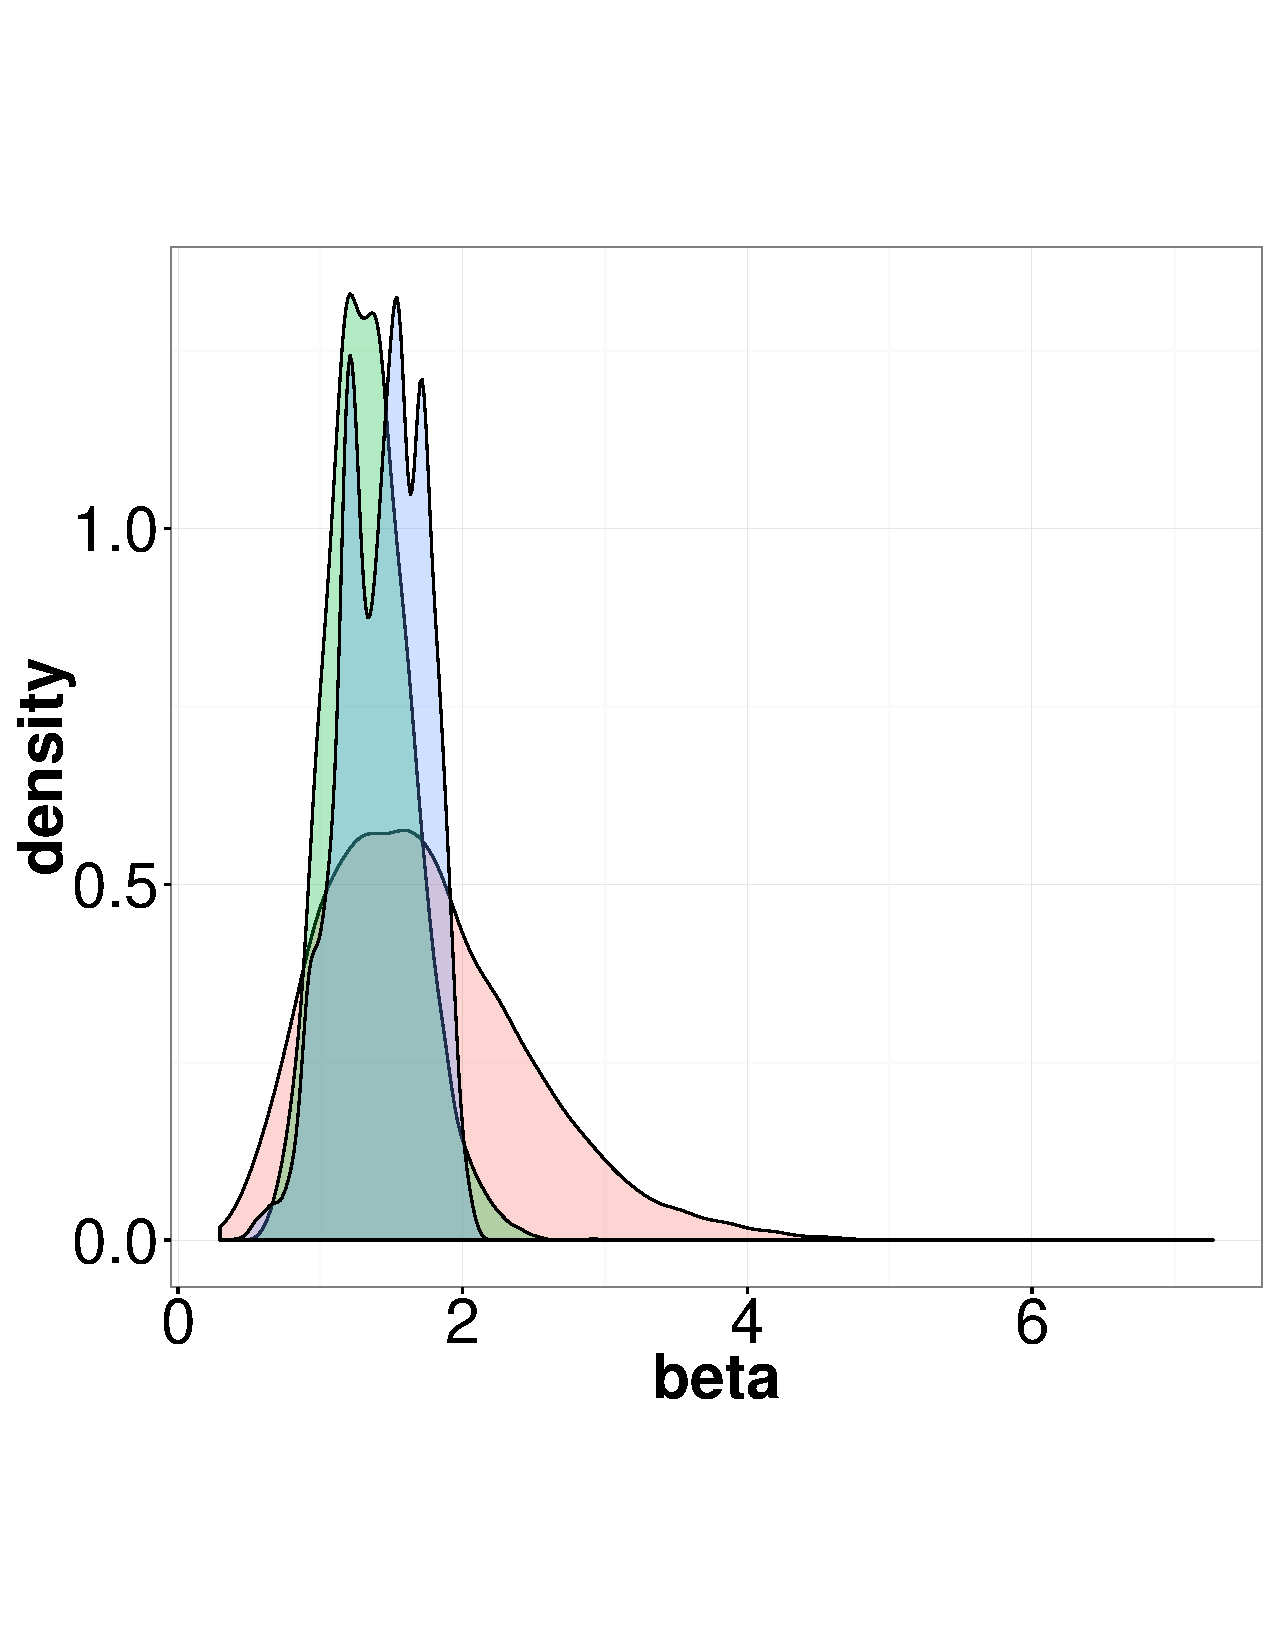
\includegraphics [width=0.98\textwidth, angle=0]{figs/dist_beta.pdf}
%   \vspace{0.2 in}
  \end{minipage}
% \begin{minipage}[!hp]{0.4\linewidth}
% \centering
%   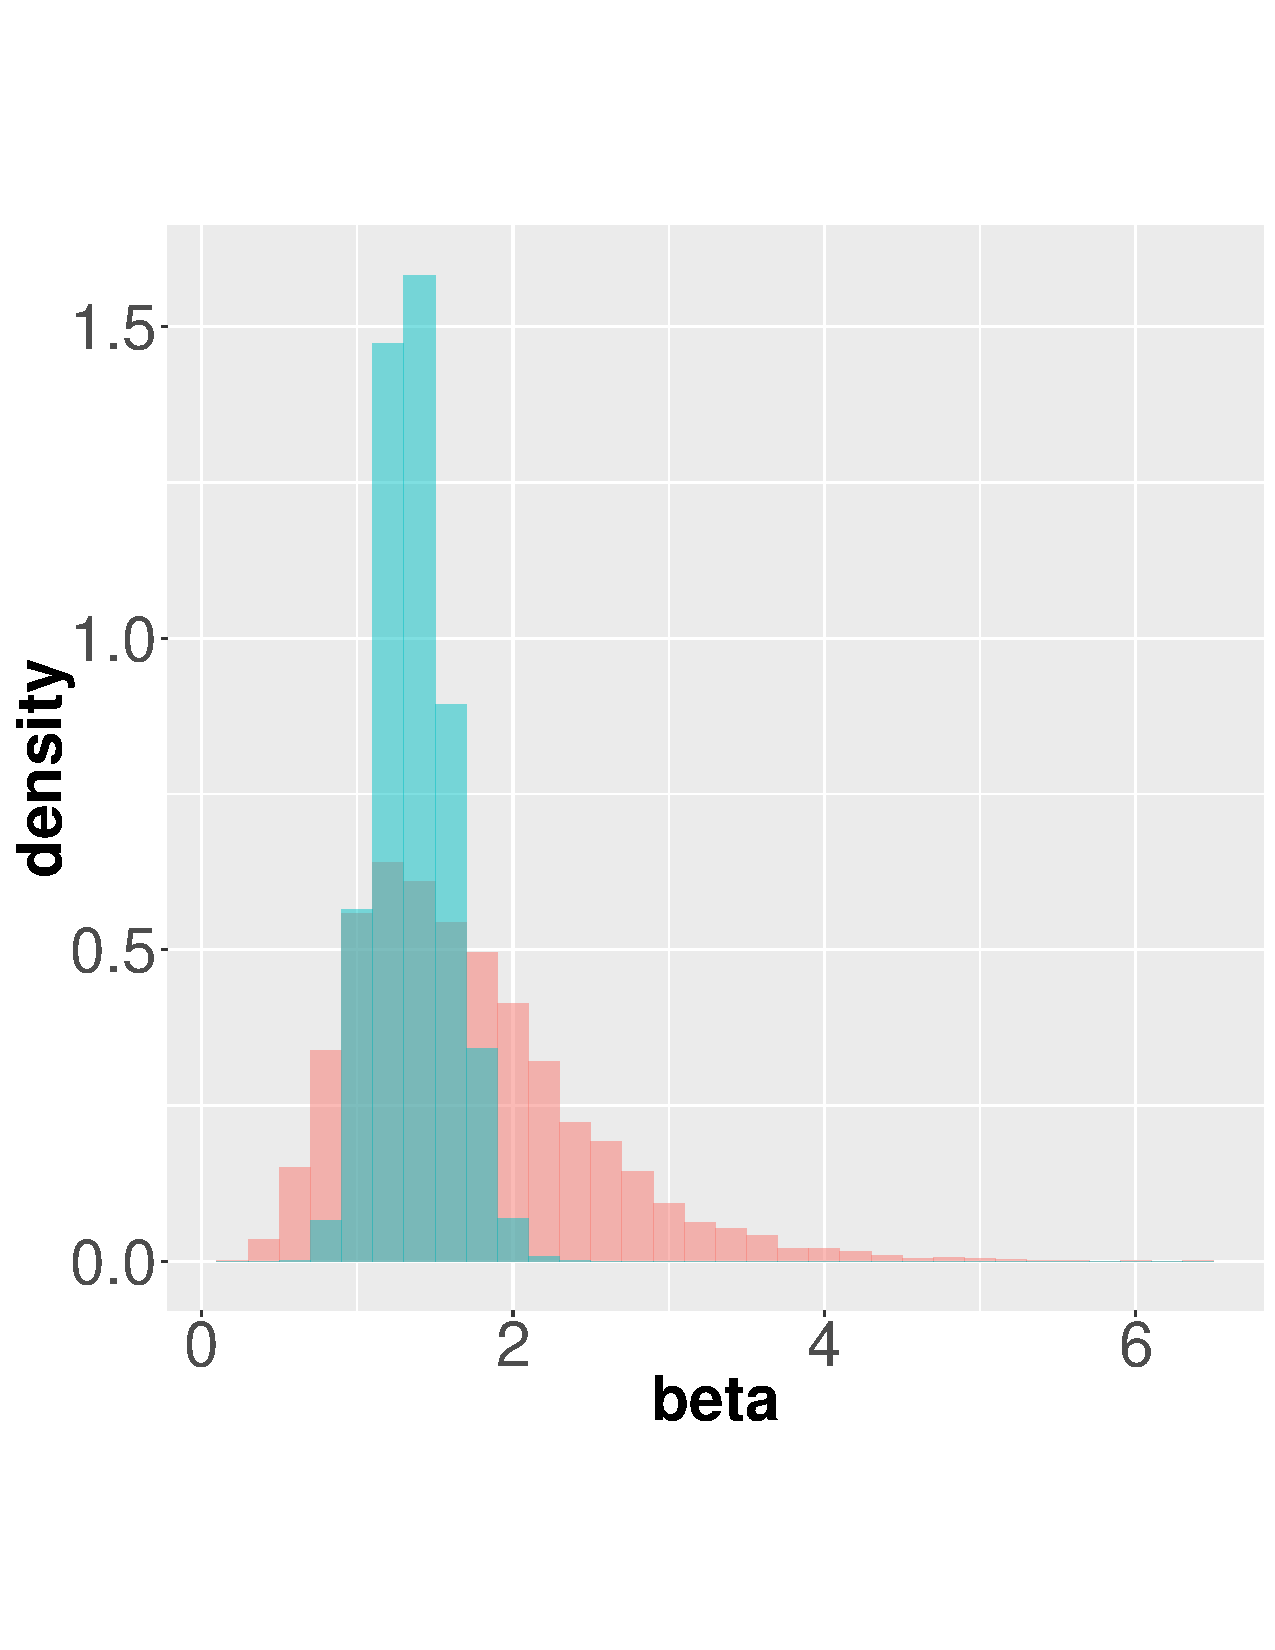
\includegraphics [width=0.90\textwidth, angle=0]{figs/hist_beta.pdf}
%   \vspace{-0 in}
% \end{minipage}
  \begin{minipage}[hp]{0.64\linewidth}
%   \vspace{-0.3 in}
  \caption{Prior distribution of an MJP parameter (the wide red density), with two conditional distributions. 
    Narrow dotted-green is the density conditioned on both the observations as well as a simulated MJP posterior. 
    The wider dashed-blue curve is density of interest: the marginal distribution of the parameters conditioned on observations. 
  Plots were produced from the experiment in section~\ref{sec:immig}.}
     \label{fig:hist}
  \end{minipage}
%   \vspace{-0.6 in}
  \end{figure}
  However, the Gibbs sampling approach coupling between path and parameters can result in a very sluggish exploration of parameter and path space. 
  We illustrate this in figure~\ref{fig:hist}~\citep[inspired by][]{papaspiliopoulos2007general}), which shows the posterior distribution of an MJP parameter (in dashed-blue) is less concentrated than the distribution conditioned on both observations as well the MJP trajectory (dotted-green). 
The coupling is strengthened as the trajectory grows longer, and the Gibbs sampler can mix very poorly for situations with long observation periods, even if the observations themselves are sparse and only mildly informative about the parameters.

% \subsection{A marginal sampler for MJP parameters} 
% For the discrete-time case, this problem of parameter-trajectory
% coupling can be circumvented by marginalizing out the MJP trajectory 
% and directly sampling from the posterior over parameters $P(\theta|X)$.
% In its simplest form (Algorithm~\ref{alg:disc_time_mh}), this 
% involves a Metropolis-Hastings scheme that proposes a new parameter 
% $\vartheta$ from some proposal distribution 
% $q(\vartheta|\theta)$, accepting or rejecting according to the usual
% Metropolis-Hastings probability. The latter step requires calculating the 
% marginal probabilities $P(X|\theta)$ and $P(X|\theta')$, integrating out
% the exponential number of possible latent trajectories. Fortunately,
% this marginal probability is a by-product of the forward-backward
% algorithm used to sample a new trajectory, so that no 
% additional computational burden is involved. 
% %The overall algorithm then is:
% \begin{algorithm}[H]
%   \caption{Metropolis-Hastings parameter inference for a discrete-time 
% Markov chain}
%    \label{alg:disc_time_mh}
%   \begin{tabular}{l l}
%    \textbf{Input:  } & \text{Observations $X$},
%    proposal density $q(\vartheta|\ctheta)$, and 
%    \text{previous parameters $\ctheta$}.\\
%    \textbf{Output:  }& \text{A new Markov chain parameter $\ntheta$}.\\
%    \hline
%    \end{tabular}
%    \begin{algorithmic}[1]
%   \State Propose a new parameter $\vartheta$ from the proposal distribution
%   $q(\vartheta|\ctheta)$.
%   \State Run the forward pass of the forward-backward algorithm to 
%     obtain the marginal likelihood of the observations, $P(X|\vartheta)$.
%     \State Set $\ntheta = \vartheta$ with probability 
%     $\min(1,\frac{P(X,\vartheta)q(\ctheta|\vartheta)}{P(X,\ctheta)q(\vartheta|\ctheta)})$, else 
%     $\ntheta = \ctheta$.
%   \State Sample a new path with
%     the backward pass of the forward-backward algorithm.
%     %for the chosen parameter.
% \end{algorithmic}
% \end{algorithm}

% %\vspace{-.35in}
% Constructing a marginal sampler over the MJP parameters by
% integrating out the continuous-time trajectory is harder.
% %the set of transition times is unbounded, with individual elements
% %unconstrained over the observation interval $[0,\cT]$.
% %Naively calculating this marginal probability for the continuous-time
% %case is not straightforward, as there is no finite set of candidate
% %times to make a pass over. 
% One approach~\citep{FearnSher2006} makes a sequential 
% forward pass through all {\em observations} $X$, using matrix exponentiation
% to marginalize out all
% continuous-time paths between successive times. As
% shown in~\cite{RaoTeh13}, this approach is cubic rather than 
% quadratic in the 
% number of states, cannot exploit structure like sparsity in the 
% transition matrix, and can depend in not trivial ways on the exact 
% nature of the observation process.
% Also, the number of expensive matrix exponentiations depends on
% the number of observations rather than the number of transitions.
% %
% %
% A second approach, particle MCMC~\citep{Andrieu10}, uses 
% particle filtering to get an unbiased estimate of the marginal 
% $P(X|\theta)$. Plugging this into the Metropolis-Hastings 
% acceptance probability results in an MCMC sampler that targets the 
% correct posterior, however %~\cite{Andrieu09}, 
% the resulting scheme does not exploit the structure 
% of the MJP, and we show that it is quite inefficient.

% The advantage of introducing the thinned events $U$ was demonstrated in 
% \cite{RaoTeh13, RaoTeh12} : this allows exploiting discrete-time 
% algorithms like FFBS for path sampling.
% %be brought to playthe thinning-based approach over matrix exponential and particle-MCMC
% %approaches for trajectory inference. 
% In the next section, we outline a \naive\  first attempt at extending this 
% approach to 
% parameter inference.
% We describe why this approach is not adequate, and then describe our
% final algorithm. % in the section after. 

\vspace{-.2in}
\section{\Naive\ parameter inference via Metropolis-Hastings}
%A natural approach to reduce the coupling in the Gibbs sampler is to reduce ?Bayesian fraction of missing information?. 
For discrete-time HMMs, path-parameter coupling can be circumvented by marginalizing out the Markov trajectory, and directly sampling from the marginal posterior $P(\theta|X)$.
In its simplest form, this involves a Metropolis-Hastings (MH) scheme that proposes a new parameter $\vartheta$ from some proposal distribution $q(\vartheta|\theta)$, accepting or rejecting according to the usual MH probability.
The marginal probabilities over $X$ given parameters are computed using the FFBS algorithm.
The Rao-Teh algorithm, which recasts posterior simulation for continuous-time models as discrete-time simulation on a random grid, then provides a simple mechanism to incorporate such an MH-scheme into continuous-time settings: directly update $\theta$, conditioning on the random grid $W$, but marginalizing out the states $(v_0, V)$.
%, following the scheme from Algorithm~\ref{alg:disc_time_mh}.
%The resulting scheme updates $\theta$ conditioned on the random 
%grid, but with the trajectory integrated out 

Specifically, given $\theta$ and the Poisson grid $W$, rather than simulating new path values (the backward pass in algorithm~\ref{alg:Unif_gibbs}), and then conditionally updating $\theta$ (the second step in algorithm~\ref{alg:MJP_gibbs}), we {\em first} propose a parameter $\vartheta$ from $q(\vartheta|\theta)$. This is accepted with probability 
$$ \texttt{acc} = \min\left(1, 
\frac{P(X|W,\vartheta) P(W|\vartheta)P(\vartheta)q(\theta|\vartheta)} {P(X|W,\theta) P(W|\theta)P(\theta)q(\vartheta|\theta)}\right),$$ 
%Only after accepting or rejecting do we simulate state values via a backward pass.
thereby targeting the distribution $P(W,\theta|X)$.
In the equation above, $P(X|W,\theta)$ is the probability of the observations $X$ given $W$ with $(v_0,V)$ marginalized out. 
Uniformization says this is the marginal probability of $X$ under a discrete-time HMM on $W$, with transition matrix $B(\theta)$. This can be computed using the forward pass of FFBS algorithm (steps 4 and 6 of algorithm~\ref{alg:MH_naive}). 
The term $P(W|\theta)$ is the probability of $W$ under a rate-$\Omega(\theta)$ Poisson process. 
These, and the corresponding terms for $\vartheta$ allow the acceptance probability to be computed.
%make a forward pass over $W$, and calculate and $P(X|W,\vartheta)$. % as in algorithm~\ref{alg:disc_time_mh}.
Only {\em after} accepting or rejecting $\vartheta$ do we simulate new states $(v'_0,V')$, using the new parameter $\theta'$ in a backward pass over $W$. 
%Then discard all self-transitions, resample $W$ and repeat. 
The new trajectory and parameter are used to simulate a new grid $W'$, and the process is repeated.
Algorithm~\ref{alg:MH_naive} includes all the details of this algorithm, with figure~\ref{fig:naive_mh} in the appendix sketching out the main idea.

%\vspace{-.1in}
%\vspace{-.32in}
\begin{algorithm}[H]
   \caption{\Naive\  MH for parameter inference for MJPs }
   \label{alg:MH_naive}
  \begin{tabular}{l l}
   \textbf{Input:  } & \text{Observations $X$}, 
                       \text{the MJP path $S(t) = (s_0, S, T)$, the  parameters $\theta$ }and $\pi_0$.\\ 
      %               & \text{A  Metropolis-Hasting proposal $q(\cdot | \theta)$}.\\
   \textbf{Output:  }& \text{A new MJP trajectory $S'(t) = (s'_0, S', T')$, 
                            new MJP parameters $\theta'$}.\\
   \hline
   \end{tabular}
   \begin{algorithmic}[1]
     \State Set $\Omega(\theta) > \max_s{A_s(\theta)}$ for
     some function $\Omega(\cdot)$, e.g.\ $\Omega(\theta) = 
      2\max_s A_s(\theta)$.
      \State \textbf{Simulate the thinned times $U$} from a rate-$(\Omega(\theta)-A_{S(t)}(\theta))$ Poisson process: 

      $\qquad \qquad \qquad \qquad U \sim \text{PoissProc}(\Omega(\theta) - A_{S(t)}(\theta)).$

      \State 
      Set $W = T \cup U$ and discard $(s_0,S)$. Define $\tilde{W} = 0 \cup W \cup t_{end}$.
    \State 
    \textbf{Forward pass:}
    Set $B(\theta) = I + \frac{1}{\Omega(\theta)}A(\theta)$ and
    $\fwd^\theta_0(\cdot) = \pi_0$.
 %   Sequentially update $\fwd^\theta_i(\cdot)$ at time $w_i \in W$ as: 
\vspace{-.1in}
    $$\textbf{for } i=1\rightarrow |\tilde{W}|\textbf{ do:} \quad \fwd^{\theta}_i(s') = \sum_{s \in \cS} \ell_{i-1}(s) \cdot \fwd^\theta_{i-1}(s)\cdot B_{ss'}(\theta), \quad \forall s' \in \cS.\qquad\qquad\quad $$
    \State \textbf{Propose $\vartheta \sim q(\cdot| \theta)$.}
    For all elements of $\tilde{W}$, calculate $\fwd^\vartheta_i(\cdot)$ similar to above.
      \State \textbf{Accept/reject:} 
      Set $P(X|W,\theta) = \sum_{s \in \cS} \fwd_{|\tilde{W}|}^\theta(s),$ $P(W|\theta) = \Omega(\theta)^{|W|}\exp(-\Omega(\theta)t_{end})$, with similar expressions for $\vartheta$. 
      With probability $\texttt{acc}$, set $\theta'$ to $\vartheta$, else set it to $\theta$, where: %Here 
      %The acceptance probability for $\vartheta$ is given by 
%         \vspace{-.05in}
          \begin{align}
            \label{eq:ncp_acc}
            \texttt{acc} &=  1 \wedge \frac{P(\vartheta|W, X)}{P(\theta|W, X)} \frac{q(\theta|\vartheta)}{q(\vartheta|\theta)}
          =  1 \wedge \frac{P(X| W,\vartheta) P(W | \vartheta)P(\vartheta)}
            {P(X|W, \theta)P(W | \theta)P(\theta)} \frac{q(\theta|\vartheta)}{q(\vartheta|\theta)}.
          \end{align}
%         \vspace{-.1in}
          %$P(X|W,\vartheta) = \sum_{s \in \cS} \fwd_{|W|}^\vartheta(s) $. Use these, and the fact that $P(W|\theta)$ is Poisson-distributed to accept or reject the proposed $\vartheta$. Write the new parameter as $\theta'$.
    %as \boqian{$(W,\theta,\vartheta)$}.
    \State %For the new parameter $\theta'$, simulate states $V$. 
    \textbf{Backward pass:}
    Set $v_{|W|} \sim \bck^{\theta'}_{|W|}(\cdot)$, where $\bck^{\theta'}_{|W|}(s) \propto \fwd^{\theta'}_{|W|}(s)\cdot\ell_{|W|}(s) \quad \forall s \in \cS.$ 
    %at time $w_i$ given $v_{i+1}$  at time $w_{i+1}$:
\vspace{-.1in}
    $$ \textbf{for } i=(|W|-1)\rightarrow 0\textbf{ do:} \quad v_i \sim \bck^{\theta'}_i(\cdot),\ \ \text{where } 
    \bck^{\theta'}_i(s) \propto \fwd^{\theta'}_i(s)\cdot B_{sv_{i+1}}(\theta') \cdot \ell_i(s)  \ \forall s \in \cS.$$
   % Here, $\bck^{\theta'}_{|W|}(\cdot) = \fwd^{\theta'}_{|W|}(\cdot)$.  This completes the FFBS algorithm.
    \State Set $s'_0=v_0$. Let $T'$ be the set of times in $W$ when $V$ changes state. Define $S'$ as the corresponding set of state values. Return $(s'_0, S', T', \theta')$.
\end{algorithmic}
\end{algorithm}
\vspace{-.1in}
The resulting MCMC algorithm updates $\theta$ with the MJP trajectory 
integrated out, and by instantiating less `missing' information, can be expected to mix better. 
This can be quantified by the so-called Bayesian fraction of missing information~\citep{liu1994fraction, papaspiliopoulos2007general}. 
The Gibbs sampler of algorithm~\ref{alg:MJP_gibbs} can be viewed as operating on a centered parametrization~\citep{papaspiliopoulos2007general} or sufficient augmentation~\citep{yu2011center} of a hierarchical model involving $\theta$, the Poisson events $W$, and the state values $(v_0,V)$. The MH algorithm reverses the order in which the path and parameter are updated, and is closely related to noncentered parametrizations or ancillary augmentations. 
For a detailed review of the suitability of these two approaches, as well as ways to combine them together, we refer to~\citet{papaspiliopoulos2007general, yu2011center}.

We note that even with the state values $(v_0,V)$ marginalized out, $\theta$ is updated {\em conditioned on $W$}. 
The distribution of $W$ depends on $\theta$: $W$ follows a rate-$\Omega(\theta)$ Poisson process. This dependence manifests in the $P(W|\theta)$ and $P(W|\vartheta)$ terms in equation~\eqref{eq:ncp_acc}. 
The fact that the MH-acceptance involves the probability of the observations  $X$ is inevitable, however the $P(W|\theta)$ term is an artifact of the computational algorithm of Rao-Teh. 
In our experiments, we show that this term significantly affects acceptance probabilities and mixing. 
For parameter $\theta$, $|W|$ is Poisson distributed with mean and variance $\Omega(\theta)$. 
If the proposed $\vartheta$ is such that $\Omega(\vartheta)$ is half $\Omega(\theta)$, then the ratio $P(W|\vartheta)/P(W|\theta)$ will be small, and $\vartheta$ is unlikely to be accepted. 
%, resulting in a low acceptance probability.  
This will slow down mixing.
The next section describes our main algorithm that gets around this.


\section{An improved Metropolis-Hasting algorithm}
\vspace{-.05in}
Our main idea is to symmetrize the probability of $W$ under the old and 
proposed parameters, so that 
$P(W|\theta)$ disappears from the acceptance ratio. This results
in a significantly more efficient, and also a simpler MCMC scheme.
%This forms the main contribution of this paper.
As before, the MCMC iteration begins with the pair $(S(t), \theta)$. 
Instead of simulating the Poisson events $U$, we first generate a new 
parameter $\vartheta$ from $q(\vartheta|\theta)$. Treat this as an 
auxiliary variable, so that the augmented space now is the triplet 
$(S(t), \theta,\vartheta)$. We pretend $S(t) \equiv (S,T)$ was sampled by  
uniformization, where the dominating Poisson rate $\Omega$ equals 
$(\Omega(\theta) + \Omega(\vartheta))$ instead of just $\Omega(\theta)$ 
(recall any choice greater than $\max_s A_s$ is valid).
Now the set of thinned events $U$ is piecewise-constant
Poisson with intensity $\Omega(\theta) + \Omega(\vartheta) - 
A_{S(t)}$. Following algorithm~\ref{alg:Unif_gibbs} or~\cite{RaoTeh13}, 
the {\em a priori} probability of the reconstructed set $W = U \cup T$, 
$P(W|\theta,\vartheta)$, is a homogeneous Poisson 
%the union of $U$ with the actual trajectory transition times $T$, 
process with rate $\Omega(\theta) + \Omega(\vartheta)$. Discard all 
MJP state information, so that the MCMC state space is $(W, \theta, \vartheta)$,
and propose swapping $\theta$ with $\vartheta$. 
Observe from
symmetry that the Poisson skeleton $W$ has the same probability both
before and after this proposal, so that unlike the previous scheme,
the ratio $P(W|\vartheta)/P(W|\theta)$ equals $1$.  This simplifies 
computation, and significantly improves mixing.
The acceptance probability 
%depends only on the probability of the observations
%under both set of parameters, %as we can use the forward-backward algorithm
%to calculate this. Our acceptance probability 
equals
$ 
  \min\left(1, \frac{P(X,\vartheta)q(\theta|\vartheta)}
   {P(X,\theta)q(\vartheta|\theta)}\right) = 
  \min\left(1, \frac{P(X|\vartheta)p(\vartheta)q(\theta|\vartheta)}
   {P(X|\theta)p(\theta)q(\vartheta|\theta)}\right).
   $
   The terms $P(X|\vartheta)$ and  $P(X|\theta)$ can be calculated by 
   running a forward pass of the forward-backward algorithm, and after
   accepting or rejecting the proposal, a new trajectory is sampled by
   completing the backward pass. Finally, the thinned events are
   discarded. We sketch out our algorithm in Algorithm~\ref{alg:MH_improved}
   and figure~\ref{fig:MH_improved} in the appendix. 
\begin{algorithm}[H]
   \caption{Symmetrized MH for parameter inference for MJPs }
   \label{alg:MH_improved}
  \begin{tabular}{l l}
   \textbf{Input:  } & \text{The observations $X$,}
                      \text{the MJP path $S(t) = (S, T)$, parameters $\theta$} and $\pi_0$.\\ 
                     & \text{A  Metropolis-Hasting proposal $q(\cdot | \theta)$}.\\
   \textbf{Output:  }& \text{A new MJP trajectory $S'(t) = (S', T')$, 
                            new MJP parameters $\theta'$}.\\
   \hline
   \end{tabular}
   \begin{algorithmic}[1]
      \State Sample $\vartheta \sim q(\cdot| \theta)$, and 
      set %$\Omega = \max_i A_i(\theta) + \max_i A_i(\theta^*)$. 
	$\Omega \assign \Omega(\theta) + \Omega(\vartheta)$ for some function 
    $\Omega(\theta) \ge \max_s A_s(\theta)$.
      %In the case of uniformization, we
      %have a single $\Omega$ for all states, with $\Omega = \max_i A_i(\theta) + \max_i A_i(\theta^*)$.
      %, with $h(\theta) > max_s{|A_s(\theta)|}$, $h(\theta^*) > max_s{|A_s(\theta^*)|}$ using some deterministic function $h$.
    \State Sample thinned jumps $U\subset[0, t_{end}]$ from a Poisson process with 
    piecewise-constant rate $R(t) = (\Omega - A_{S(t)}(\theta))$. 
    Set $W = T \cup U$ and discard MJP states.
    \State The current MCMC state-space is $(W,\theta,\vartheta)$. Propose swapping
    $\theta$ and $\vartheta$. %the new state-space is 
   %\boqian{ $(W, \vartheta, \theta)$.}
%$(W, \theta, \vartheta)$    
     The acceptance probability is given by
   % accept $\theta^*$ as $\tilde{\theta}$ with probability $\alpha$.
     \vspace{-.15in}
        \begin{align*}
        \alpha %&=  1 \wedge \frac{P(W,(\vartheta, \theta)| y)}{P(W, (\theta, \vartheta)| y)}\\
       % &=  1 \wedge \frac{P(y| W,\vartheta, \theta) P(W | (\vartheta, \theta))p((\vartheta, \theta))}{P(y| W,(\theta, \vartheta)) P(W | (\theta, \vartheta))p((\theta, \vartheta))}\\
        &=  1 \wedge \frac{P(X| W,\vartheta,\theta)p(\vartheta)q(\theta|\vartheta)}
        {P(X| W,\theta, \vartheta)p(\theta) q(\vartheta|\theta)}.
        \end{align*}
    \State For both $\theta$ and $\vartheta$, make a forward pass through the 
    elements of $W$, sequentially updating the distribution over states at 
    $w \in W$ given observations up to $w$. At the end, we have calculated
    $P(X|W,\theta, \vartheta)$ and $P(X|W,\vartheta, \theta)$. Use these to accept or reject the
    proposed swapping of $\theta$ and $\vartheta$. Write the new state-space
    as $(W,\theta',\vartheta')$.
    \State For the new transition matrix $B(\theta',\vartheta')$, make a backward pass through 
    the elements of
    $W$, sequentially assigning a state to each element $w_i \in W$ given 
    $w_{i+1}$.
%    Sample a path $\tilde{V}$, from a discret-time Markov chain with $|W| + 1$ steps, using FFBS algorithm. The transition matrix of the Markov chain is $B = (I + \frac{A(\tilde{\theta})}{\Omega})$ while the initial distribution over states is $\pi_0$. The likelihood of state $s$ at step $i$ is 
%    $$ L_i(s) = P(Y_{[w_i, w_{i + 1})} | S(t) = s \; for\; t \in [w_i, w_{i + 1})) = \prod_{j: t_j \in [w_i, w_{i + 1})}p(y_{t_j} | S(t_j) = s).$$\\
%%(i.e. $V(i) \sim P(V |  \theta(i), W(i - 1), y).$) Then delete all the virtual jumps to get $S(i), T(i) .$\\
    \State Let $T'$ be the set of times in $W$ when the Markov chain changes state. Define $S'$ as the corresponding set of state values. Return $(S', T', \theta')$.
\end{algorithmic}
\end{algorithm}




\section{Verifications of Algorithm 1}
\label{sec:verify}
Proof of Algorithm 1:\\
\noindent Assume: $S = [S_0,S_1, ...,S_N] \;, T = [T_0, T_1,...,T_N, T_{N+1}(T_{end})]$, and y as observations.\\
In JMLR-2013 Fast MCMC Sampling for MJP and Extensions, the FFBS frame contains $\alpha_t$ as follows.\\
Since after uniformization, the virtual jumps are added.  Then the state process of the trajectory with virtual jumps is just a discrete time markov jump process. The key point is that we need to have $W$ be conditioned, to get the marginal probability $P(y_{[T_0, T_{N + 1})} | \theta, W)$ from FFBS algorithm. \\
\begin{align*}
\alpha^\theta_t(s) = P(S_t = s\;, y_{[T_0, T_t)}, U, T).\\
P(y_{[T_0, T_{N + 1})} | \theta, W) = \sum_{s = 0}^{N-1} \alpha^\theta_N(s) \cdot P(y_{[T_N, T_{N+1})} | S_N = s).\\
P(\theta, W| y) \propto P(\theta, W, y) = P(y| W, \theta) P(W | \theta) P(\theta).
\end{align*}
$P(y|W, \theta)$ is the marginal probability we get after Forward Filtering Algorithm and the $P(W | \theta)$ is the probability density for the $poisson(\Omega)$, because of the uniformization procedure.
Let denote the kernel for (a), (b) and (c) as  $\kappa_1(\theta^*| \theta, W, T, S, y)$ , $\kappa_2(S^*, T^*|S, T, W, \theta^*, y)$ and $\kappa_3(W^*| S^*, T^*, \theta^*, y)$.\\
For Step (a) $\kappa_1(\theta^*| \theta, W, T, S)$:\\
 \begin{align*} 
P((W, T, S, \theta) \rightarrow (W, T, S, \theta^*)) P(\theta, W | y) &=  P(\theta^*, W | y)q(\theta | \theta^*)
 \wedge P(\theta, W|y) q(\theta^*| \theta) \\&= P((W, T, S,\theta^*) \rightarrow (W, T, S,\theta)) P(\theta^*, W | y).\\
\end{align*}
Thus, $  \int ab \kappa_1(\theta^*| \theta) P(\theta, W|y) d\theta = P(\theta^*, W |y). $\\
So the stationary distribution of $\kappa_1$ is $P(\theta, W | y)$.\\
Step (b) $\kappa_2(S^*, T^*|S, T, W, \theta^*, y)$: \\ 
Step(b) is the same as Fast MJPs Gibbs sampling scheme.   \\
\begin{align*}
((S, T, \theta, W) \rightarrow (S^*, T^*,\theta, W)|  y) = P(V^* | W, \theta, y) = P(V^* | W, \theta, y) / P(W, \theta, y) \end{align*}
\begin{align*}
P((S, T) \rightarrow (S^*, T^*)| W, \theta, y) P(S, T| W, \theta, y) &= P(V^* | W, \theta, y)P(V | W, \theta, y) \\&= P((S^*, T^*) \rightarrow (S, T)| W, \theta, y) P(S^*, T^*| W, \theta, y)
\end{align*}
\\So the stationary distribution of $\kappa_2(S^*, T^*| S,T,  W, y)$ is $P(S, T | W, \theta, y).$
Now, let's consider $\kappa_2 \circ \kappa_1(S^*, T^*, \theta^* | S, T, \theta, y, W)$.\\
\begin{align*}
((S, T, \theta, W) \rightarrow (S^*, T^*, \theta^*, W)|  y) = P((W, T, S, \theta) \rightarrow (W, T, S, \theta^*)) P((S, T, \theta^*.W) \rightarrow (S^*, T^*, \theta^*, W)| y) .
\end{align*}
The stationary distribution of $\kappa_1(S^*, T^*, U^*|S, T, U)$ is $P(S,T,U| \theta, y).$ And the stationary distribution of $\kappa_2(U^*| U)$ is $P(U| S, T, \theta, y).$ \\
\begin{align*}
&P((S, T, \theta, W) \rightarrow (S^*, T^*, \theta^*, W)|  y) P(S,T,\theta | W, y) \\&= P((W, T, S, \theta) \rightarrow (W, T, S, \theta^*))\cdot P(\theta|W,y) \cdot P((S, T, \theta^*.W) \rightarrow (S^*, T^*, \theta^*, W)| y) P(S, T | \theta , W, y) \\&=P((W, T, S, \theta^*) \rightarrow (W, T, S, \theta))\cdot P(\theta^*|W,y) \cdot P((S^*, T^*, \theta^*.W) \rightarrow (S, T, \theta^*, W)| y) P(S^*, T^* | \theta , W, y) \\&=P((S^*, T^*, \theta^*, W) \rightarrow (S, T, \theta, W)|  y) P(S,T,\theta | W, y).
\end{align*}
So the stationary distribution of $\kappa_2 \circ \kappa_1$ is $P(S, T,\theta| W,y).$\\
Obviously, $\kappa_3(W^*| W, S^*, T^*, \theta^*, y)$ has $P(W| S^*, T^*, \theta^*,y)$ as stationary distribution.\\
Therefore, $\int \kappa_3(W^*| W, S^*, T^*, \theta^*, y) P(W,S^*, T^*, \theta^*|y ) dW= P(W^*,S^*, T^*, \theta^*|y )$.\\
Thus, $\int \kappa_3 \cdot (\int \kappa_2 \circ \kappa_1\cdot P(W,S, T, \theta | y) d\theta dS dT)dW = \int \kappa_3 P(W,S^*, T^*, \theta^*|y )dW = P(W^*,S^*, T^*, \theta^*|y )$.\\
So the stationary distribution of $\kappa_3 \circ \kappa_2 \circ \kappa_1$ is $P(W^*,S^*, T^*, \theta^*|y )$.
%\end{proof}

\section{Verifications of Algorithm 2}
\label{sec:verify2}
Proof:
Our state is $(W, S, T, \theta, \theta^*)$. 
\begin{align*}
 p(y, W, S, T, \theta, \theta^*) &= p(\theta) q(\theta^* | \theta) P(S,T| \theta, \theta^*) P(W| S, T, \theta, \theta^*)P(y | S, T, \theta, \theta^*)\\
 &=p(\theta) q(\theta^* | \theta) P(S,T| \theta) P(W| S, T, \theta, \theta^*)P(y | S, T).
\end{align*}
The marginal distribution of $(y, S, T, \theta, \theta^*)$ and $(y, S, T, \theta)$ as follows.\\
\begin{align*}
 p(y, S, T, \theta, \theta^*) &= p(\theta) q(\theta^* | \theta) P(S,T| \theta, \theta^*)P(y | S, T, \theta, \theta^*)\\
 &=P(y, S, T, \theta) q(\theta^* | \theta).
\end{align*}
\begin{align*}
 p(y, S, T, \theta) &= p(\theta)P(S,T| \theta)P(y | S, T, \theta).
\end{align*}
So the conditional distribution over $\theta^*$ given $(y, S, T, \theta)$ is $q(\theta^* | \theta)$. And the conditional distribution over W given $(y, S, T, \theta, \theta^*)$  is $P(W | S, T, \theta, \theta^*)$, which is actually the distribution of Non Homogeneous Poisson Process with piecewise constant rate $h(\theta) + h(\theta^*) - A_{S(t)}(\theta)$.\\
Thus the Step 1 + Step 2 is actually equivalent to sampling from the conditional distribution $P(\theta^* , W| S, T, \theta, y)$.\\
The Step 3 + Step 4 satisfy the detailed balance condition. The reason is as follows.
\begin{align*}
&P((W, S, T, (\theta, \theta^*)) \rightarrow (W, S^*, T^*, (\theta^*, \theta))) P(S,T, (\theta, \theta^*) | W, y)\\
&= (1 \wedge \frac{P((\theta^*,\theta) | W, y)}{P((\theta,\theta^*) | W, y)})P(S^*, T^* | W, (\theta^*, \theta), y)P(S, T | W, (\theta, \theta^*), y)P((\theta, \theta^*) | W, y)\\
&= P((W, S^*, T^*, (\theta^*, \theta)) \rightarrow (W, S, T, (\theta, \theta^*))) P(S^*,T^*, (\theta^*, \theta) | W, y)
\end{align*} 
Therefore the stationary distribution of this MCMC sampler is $P(W, S, T, (\theta, \theta^*) | y)$. Thus the stationary distribution of $(S, T, \theta)$ is the corresponding marginal distribution $P(S, T, \theta | y)$.  

\section{Generic Exponential Model}~
\begin{algorithm}[!ht]
   \caption{Generic Gibbs sampling for MJPs for Gamma priors}
   \label{alg:Generic Gibbs}
\begin{algorithmic}
   \State {\bfseries Input:} observations $y_{[t_0, t_{k+1})}$
   \State Initialize, $i = 0$
   \\ (a) Set $\alpha(0), \beta(0)$ arbitrarily and set current trajectory $[S,T](0)$ arbitrarily.\\
    (b) Uniformize $[S,T](0)$, to get virtual jumps $U$.
   \Repeat
   \For{$i=1$ {\bfseries to} $N$}
    \State (a) Sample $U(i) \sim P( U | \beta(i - 1), \alpha(i - 1), S(i - 1), T(i - 1), y)$.\\	
    \State (b) Use FFBS algorithm to  sample states given all the jump times(both true jumps and virtual jumps).
(i.e. $V(i) \sim P(V |  \beta(i - 1), \alpha(i - 1), W(i ), y).$) Then delete all the virtual jumps to get $S(i), T(i) .$\\
    \State (c) Propose $\beta^* \sim q(.| \beta(i -1))$.\\
      Set $\beta(i) = \beta^*$, with probability $P_{acc} = 1 \wedge \frac{P(\beta^* |S(i), T(i))}{P(\beta(i - 1) |S(i), T(i))} \frac{q(\beta(i - 1)|\beta^*)}{q(\beta^*|\beta(i - 1))}$;\\Otherwise set $\beta(i) = \beta(i-1)$.\\	  
    \State (d) Sample $\alpha(i) \sim P(. | \beta(i), S(i), T(i), y)$.\\ It is a $Gamma(\mu + N, \lambda + \sum_{0}^NF_{S_i}(\beta)(t_{i + 1} - t_i))$ distribution actually.\\
    \EndFor
    \Until{$ i = N$ }
 \end{algorithmic}
 \end{algorithm}
  \begin{figure}[H]
  \centering
  \begin{minipage}[!hp]{0.45\linewidth}
  \centering
    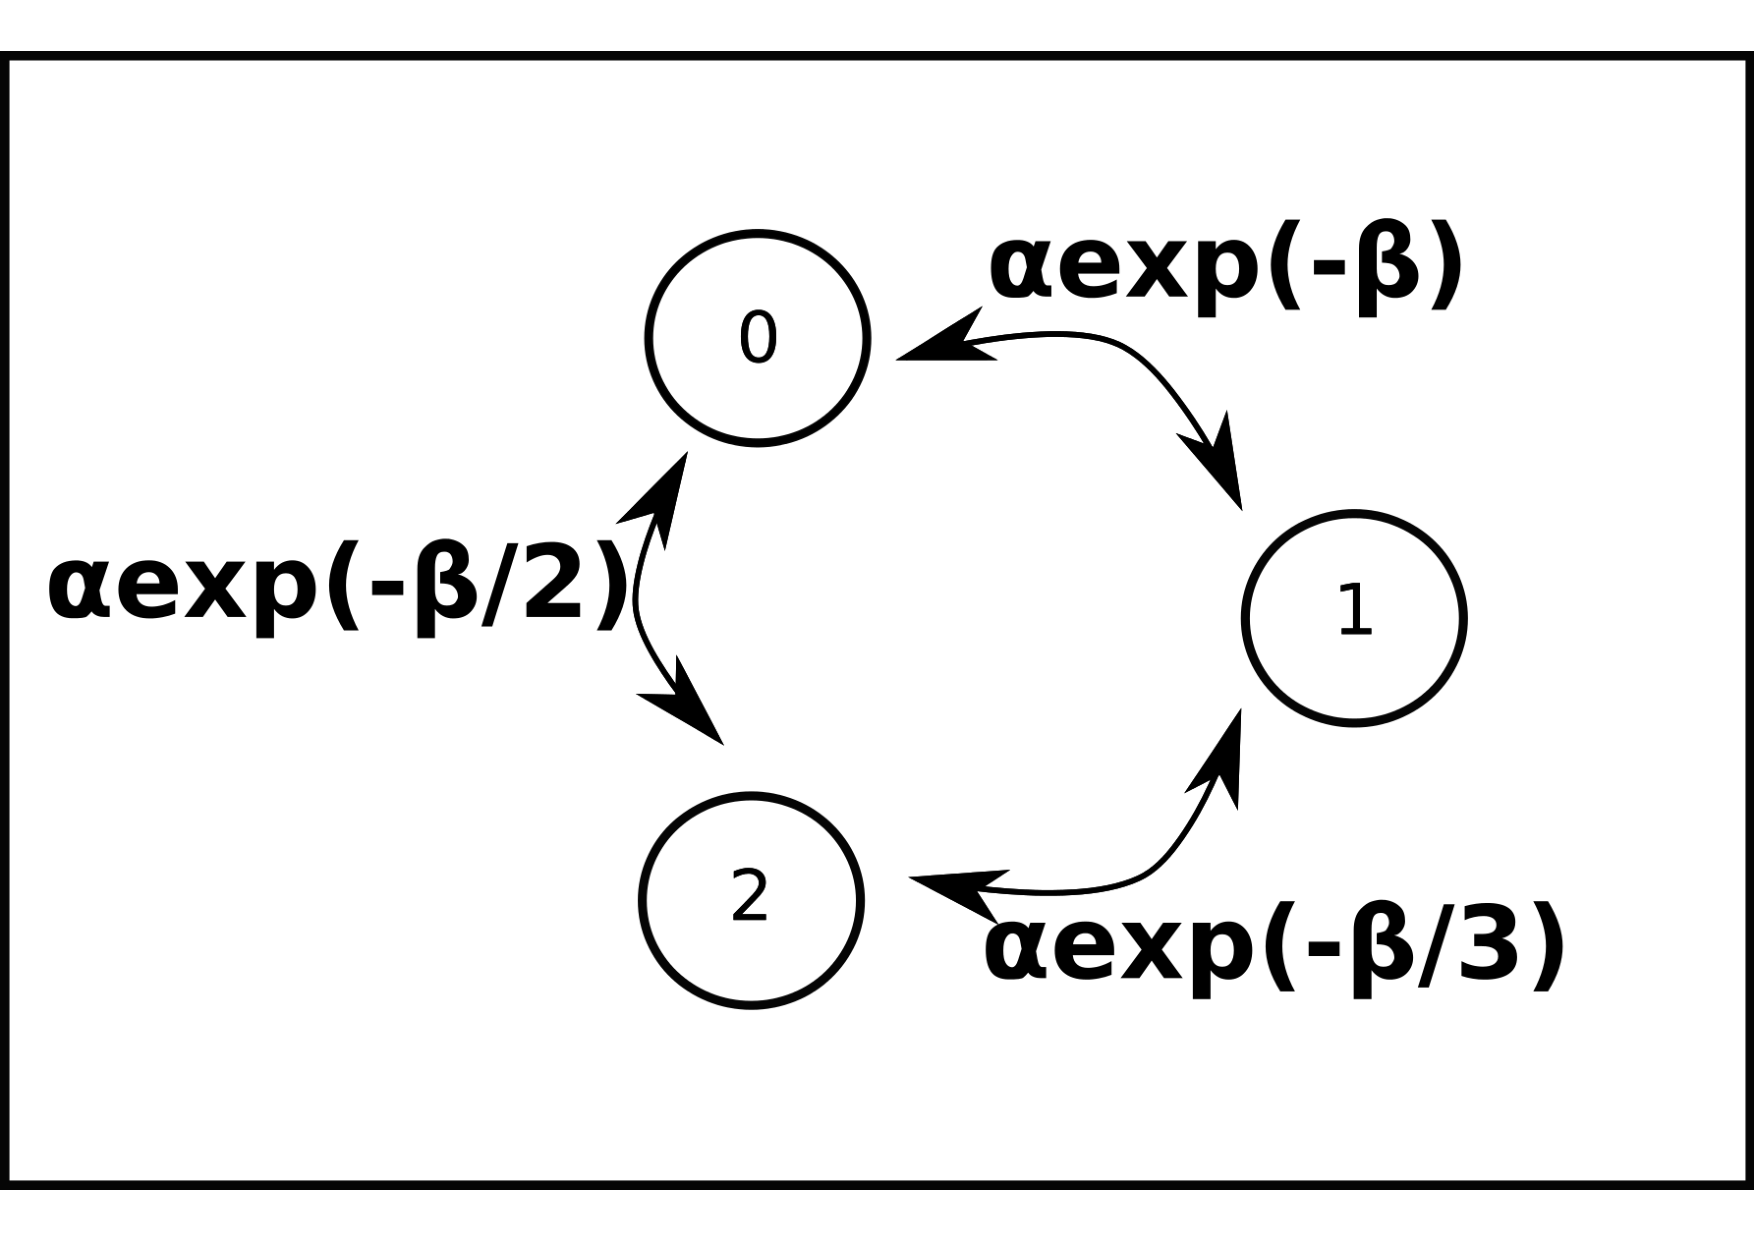
\includegraphics [width=0.70\textwidth, angle=0]{figs/exp_model.pdf}
      \end{minipage}
    \caption{exp model}
  \end{figure}

\noindent Assume: $S = [S_0,S_1, ...,S_N] \;, T = [t_0(t_{start}), t_1,...,t_N, t_{N+1}(t_{end})]$, and y as observations.\\
We consider a specific structure of rate matrix $A$. $A_{ij} = \alpha f_{ij}(\beta), \; i \neq j$. $A_{ii} = -\sum_{j \neq i} A_{ij}$. $0 \leq f_{ij} \leq 1$. Denote $F_i(\beta) = \sum_{j \neq i} f_{ij}(\beta)$.\\
\begin{align*}
P(s_0, S, T | \alpha, \beta) &= \pi_0(s_0)\prod_{i = 1}^N A_{S_{i - 1}S_i} \exp(- \int_{t_{start}}^{t_{end}} |A_{S(t)}| dt)\\
&= \pi_0(s_0) \alpha^N \prod_{i = 1}^N f_{S_{i - 1}S_i} \exp(-\alpha  \sum_{i = 0}^{N} F_{S_i}(\beta)(t_{i + 1} - t_i))\\
\end{align*}
We can assume the prior distributions of $\alpha, \beta$ are $p_1(\alpha)$ and $p_2(\beta)$.\\
Then the posterior distribution of parameters $\alpha, \beta$ will be as follows.\\
\begin{align*}
P(\alpha, \beta | s_0, S, T ) \propto \alpha^N \prod_{i = 1}^N f_{S_{i - 1}S_i} \exp(-\alpha  \sum_{i = 0}^{N} F_{S_i}(\beta)(t_{i + 1} - t_i)) p_1(\alpha)p_2(\beta)\\
\end{align*}
If we assume the priors of $\alpha$, $\beta$ are $Gamma(\mu, \lambda)$, $Gamma(\omega, \theta)$, then the posterior will have a simper form as follows. 
\begin{align*}
P(\alpha, \beta | s_0, S, T ) = C \alpha^{\mu + N - 1}\exp(-\alpha (\lambda + \sum_{i = 0}^{N} F_{S_i}(\beta)(t_{i + 1} - t_i))) \prod_{i = 1}^N f_{S_{i - 1}S_i}  \beta ^{\omega - 1} \exp(-\theta \beta)\\
\end{align*}
We notice that given $\beta,\; S,\; T$, $\alpha$ is distributed as a $Gamma$ distribution.\\
$\alpha | \beta, S, T, y  = \alpha | \beta, S, T \sim Gamma(\mu + N, \lambda + \sum_{0}^NF_{S_i}(\beta)(t_{i + 1} - t_i))$.\\
There is no conjugate distribution to sample $\beta \sim P(\beta| s_0, S, T)$. We will have to use Metropolis Hasting within Gibbs to sample $\beta$. The target distribution is the following one.
$$ P(\beta | S, T) = C \frac{\prod_{i = 1}^N f_{S_{i -1}S_i}(\beta)\beta^{\omega - 1} \exp(-\theta \beta)}{(\lambda + \sum_{i = 0}^{N} F_{S_i}(\beta)(t_{i + 1} - t_i))^{\mu + N}}.$$
Such doubling might slow the mixing of the Markov chain. We can apply our Metropolis Hasting algorithm on this model.
\subsection{Experiments}
In the following, we evaluate a Python implementation of our algorithms compared to other exact samplers which include Gibbs sampler and Particle MCMC sampler. We consider one special case when $f_{ij}(\beta) = \exp(-\beta / (i + j))$. We consider three different dimensions which are 3, 5, and 10 and three different k which are 1.5, 2, and 3. We generated random parameters $\alpha$, $\beta$ from prior distributions ($Gamma(3,2), Gamma(5, 2)$), and used these parameters to construct the transition matrix A. Then we generate an MJP trajectory with a uniform initial distribution over states and the transition matrix A. The state of this MJP trajectory was observed via a Normal distribution with mean equal to the value of state and variance 1, and the proposal kernel is a lognormal distribution with location parameter $\log(\theta_{old})$ and scale parameter$\sigma$. Posterior samples given the observations were produced by a Python implementation of our algorithm. 100 MCMC runs were performed, each run consisting of 10000 iterations except for Particle MCMC algorithm. For Particle MCMC, each run consists 3000 iterations while the number of particles can be 5, 10 or 20. We also explored the gradient information of the target distribution to apply Hamiltonian Monte Carlo with different step sizes and different numbers of leapfrog jumps. For HMC,  each run consists 20000 iterations while the numbers of leapfrog jumps can be 1, 3, 5, or 10, and the leapfrog stepsize can be  0.02, 0.05 and 0.1. For each run, the acceptance rates as well as the time spent was calculated, and effective sample sizes (ESSs) of MCMC sampling parameters) were calculated using R-CODA (Plummer et al., 2006). The overall ESS per unit time of a run is defined to be the mean ESS per unit time across all these ESSs per unit time.\\
Figure 1, 2 and 3 plot the overall  ESS per unit time against the variance of the proposal kernel per run, for different methods and different scaling parameters k($k = 1.5, 2, 3$) and different dimensions($p = 3, 5, 10$), where the  $\Omega = k \max(\Omega_{old}, \Omega_{new})$ when $k < 2$, or $\Omega = k (\Omega_{old} + \Omega_{new})$ when $k \leq 2$. We see that the improved MH algorithm is more efficient in these cases with respect to the overall ESS per unit time. We also see that increase the scaling parameter will decrease the efficiency of the improved MH algorithm respect to overall ESS per unit time, when $k > 2$. If we set $\Omega = 1.5 \max(\Omega_{old}, \Omega_{new})$, the performance of the improved MH will not be as good as the case we set $\Omega = 2(\Omega_{old} + \Omega_{new})$ when the proposal log variance is large.\\
Figure 4 shows the initial burn-in of a sampler with this setting for different initializations. The vertical axis shows the number of state transitions in the MJP trajectory of each iteration. This quantity quickly reaches its equilibrium value within a few iterations.\\

Figure 5 plots ESS per unit time a
Figure 6 plots ESS per unit time as observation interval and the number of observations both increase when the dimension is $3$ and the scaling parameter k is $2$. Gibbs sampler decreases faster than Metropolis Hasting Method, due to the doubling of MJP paths and the parameters. \\

Figure 7 plots ESS per unit time as observation interval increases with number of observations fixed, when the dimension is $3$ and the scaling parameter k is $2$.Gibbs sampler decreases faster than Metropolis Hasting Method, due to the doubling of MJP paths and the parameters. In addition Gibbs sampler decreases even more faster than previous case when the number of observations is not fixed. \\

Figure 8 plots ESS plots the overall  acceptance rate against the log variance of the proposal kernel per run for dimension $3$. 


  \begin{figure}%[b]
  \centering
  \begin{minipage}[!hp]{0.45\linewidth}
  \centering
    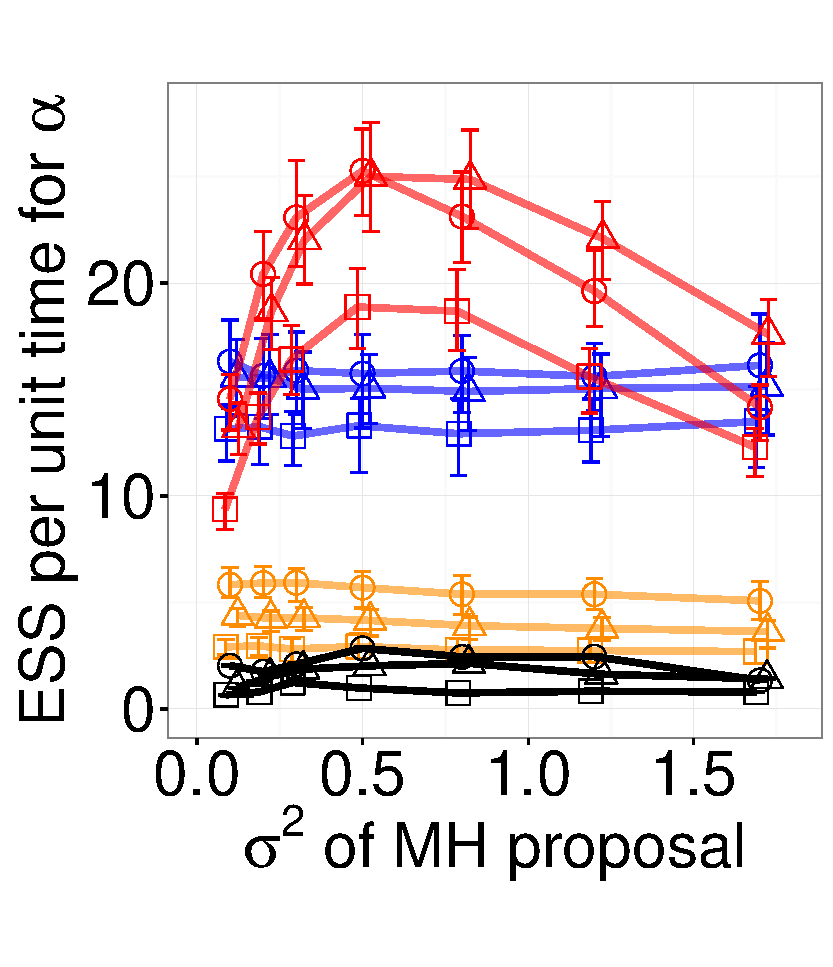
\includegraphics [width=0.70\textwidth, angle=0]{figs/exp_3_alpha.pdf}
      \end{minipage}
  \begin{minipage}[hp]{0.45\linewidth}
  \centering
    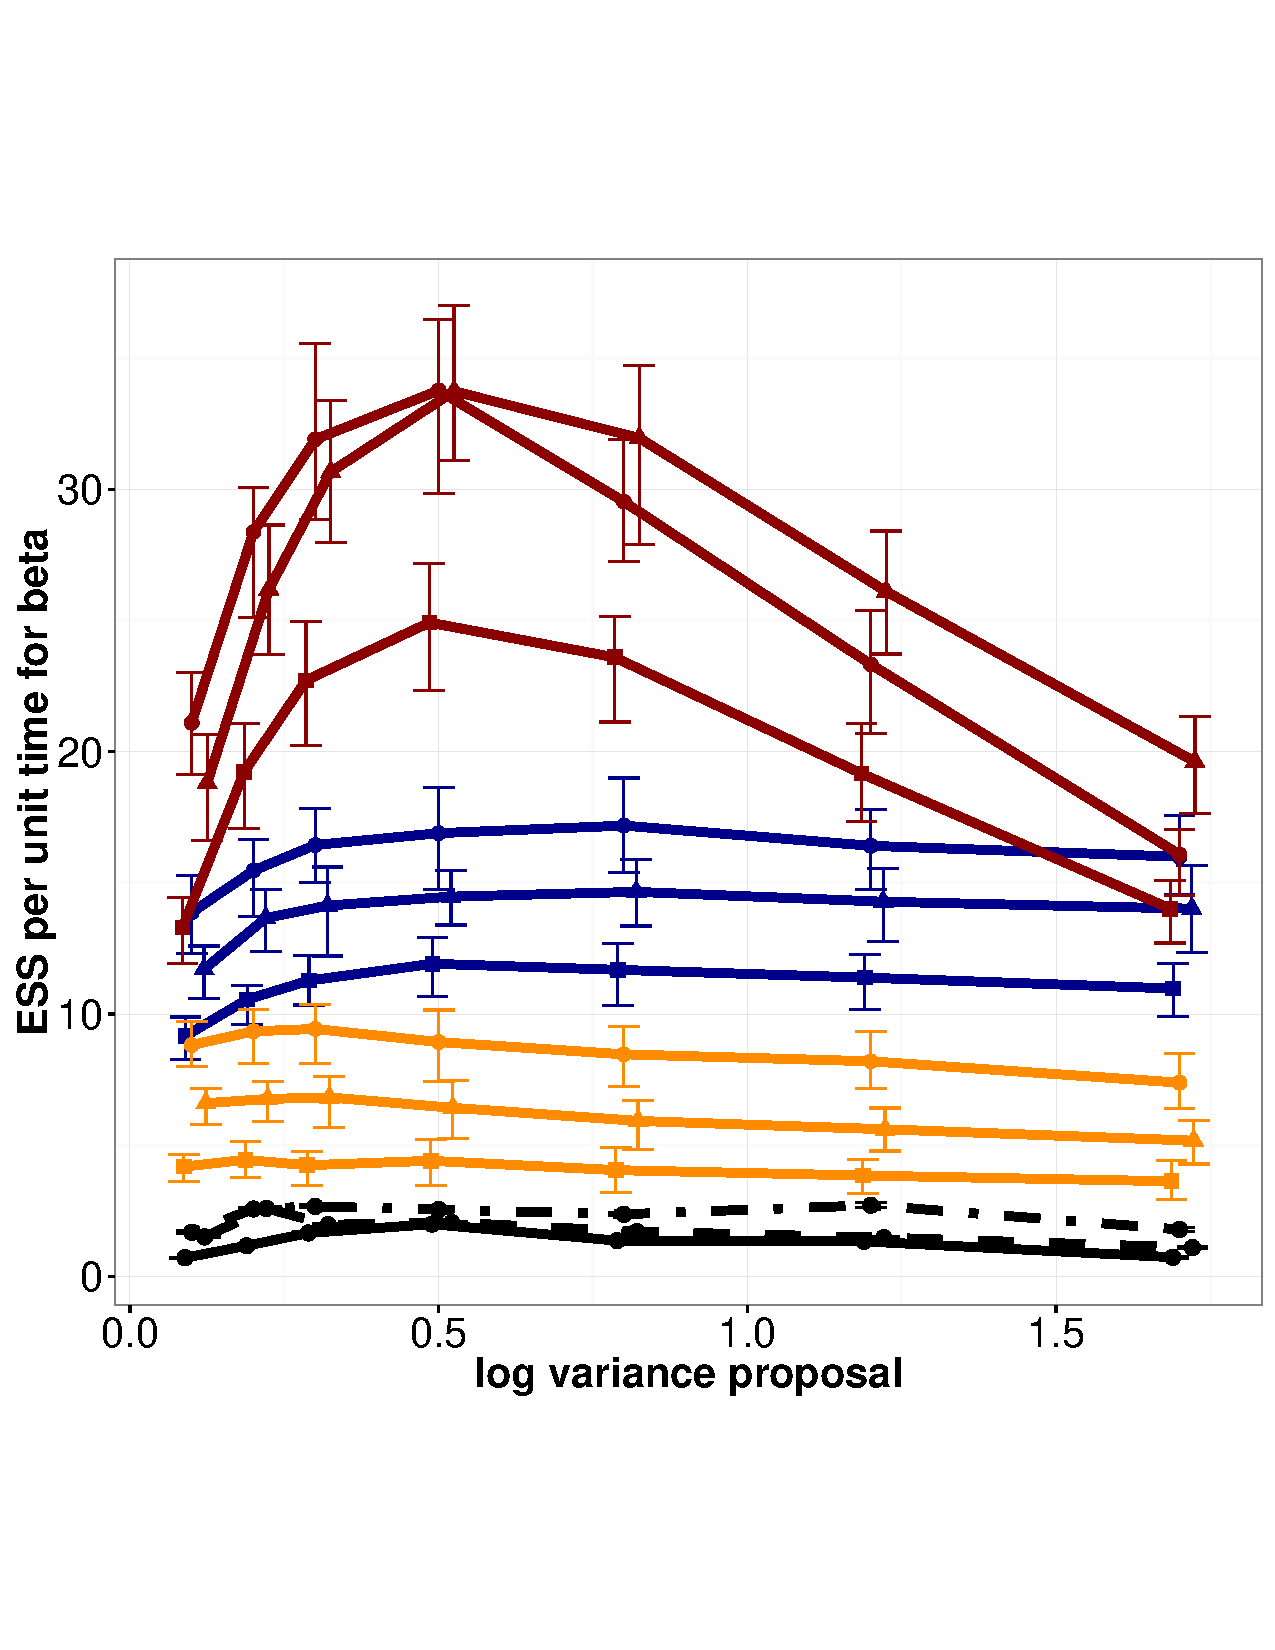
\includegraphics [width=0.70\textwidth, angle=0]{figs/exp_3_beta.pdf}
    \vspace{-0 in}
%    \caption{ESS/sec for exp model (beta, dim 3)}
     \label{fig:ESS_EXP_D3}
  \end{minipage}
    \caption{ESS/sec for exp model (dim 3). The left is for $\alpha$, and the right is for $\beta$.}
  \end{figure}
  \begin{figure}[H]
  \centering
  \begin{minipage}[hp]{0.45\linewidth}
  \centering
    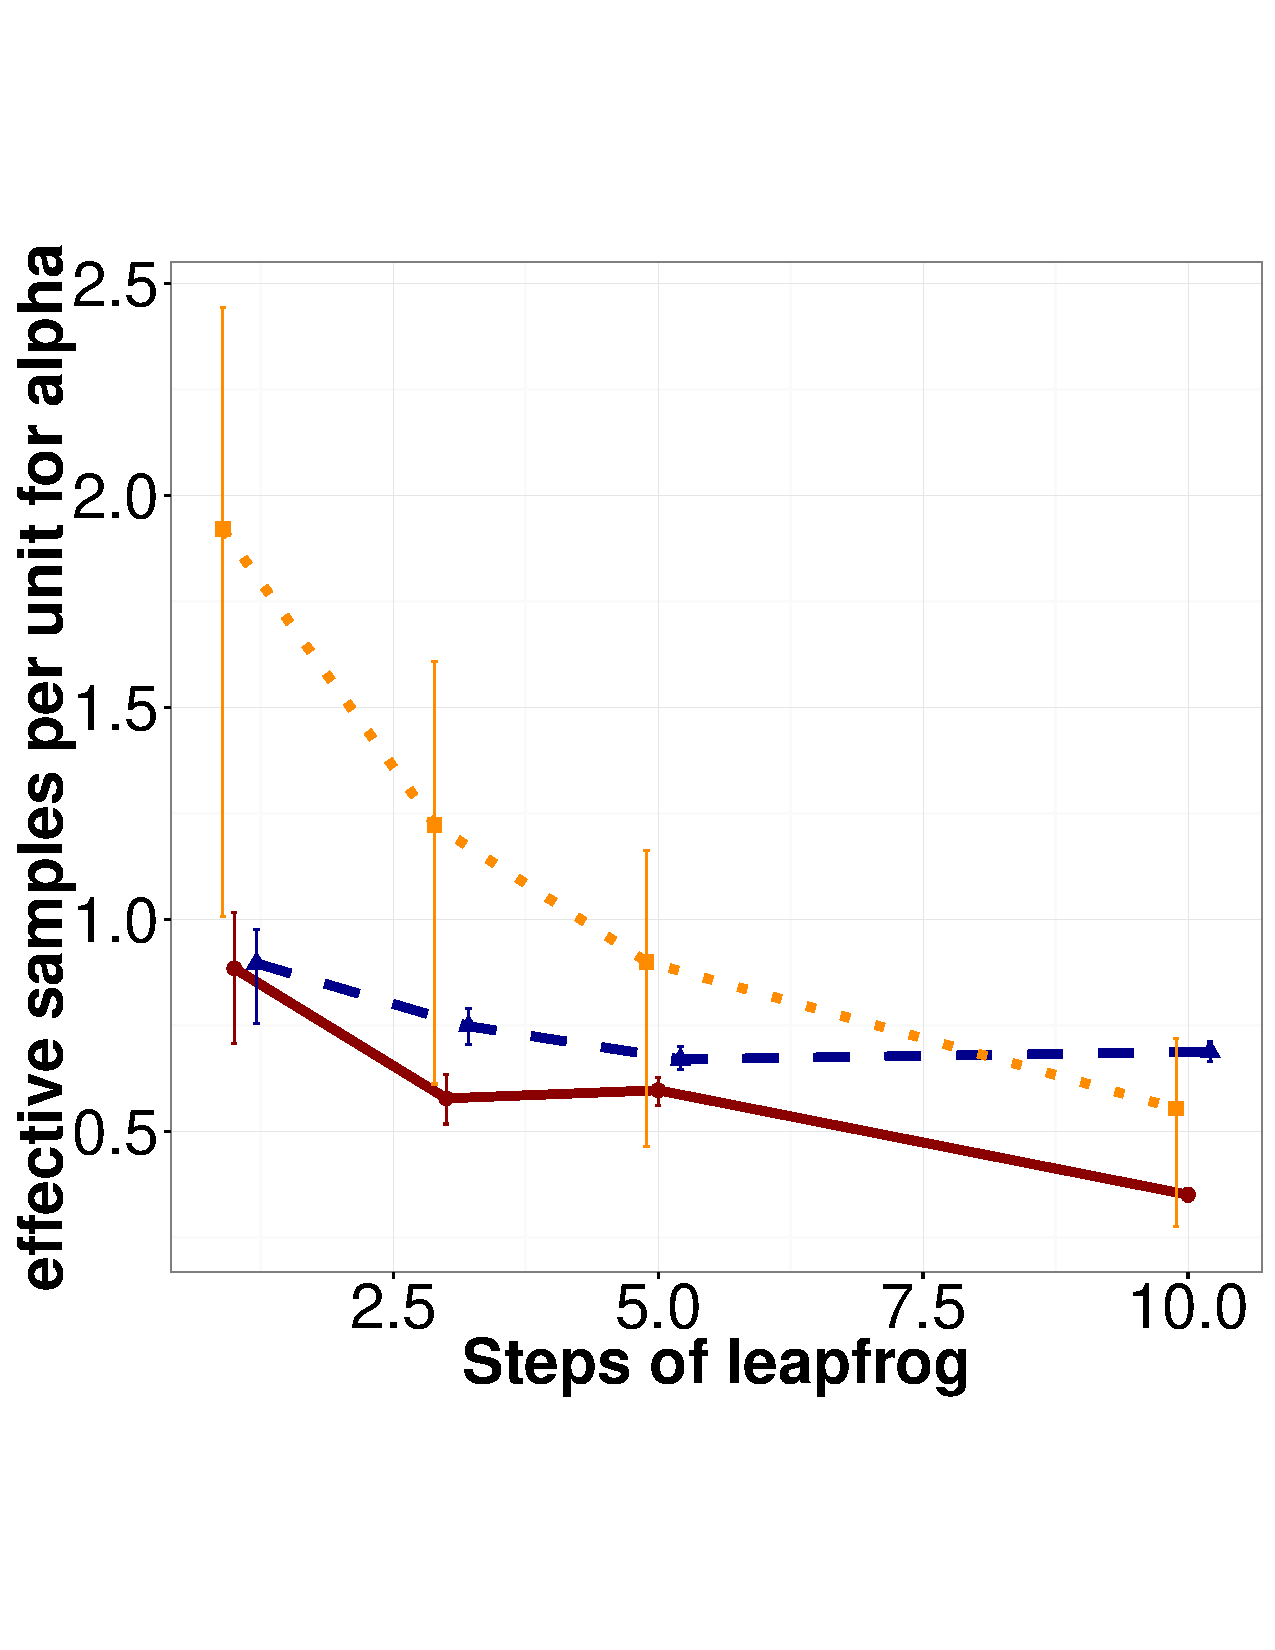
\includegraphics [width=0.70\textwidth, angle=0]{figs/h_alpha.pdf}
      \end{minipage}
  \begin{minipage}[hp]{0.45\linewidth}
  \centering
    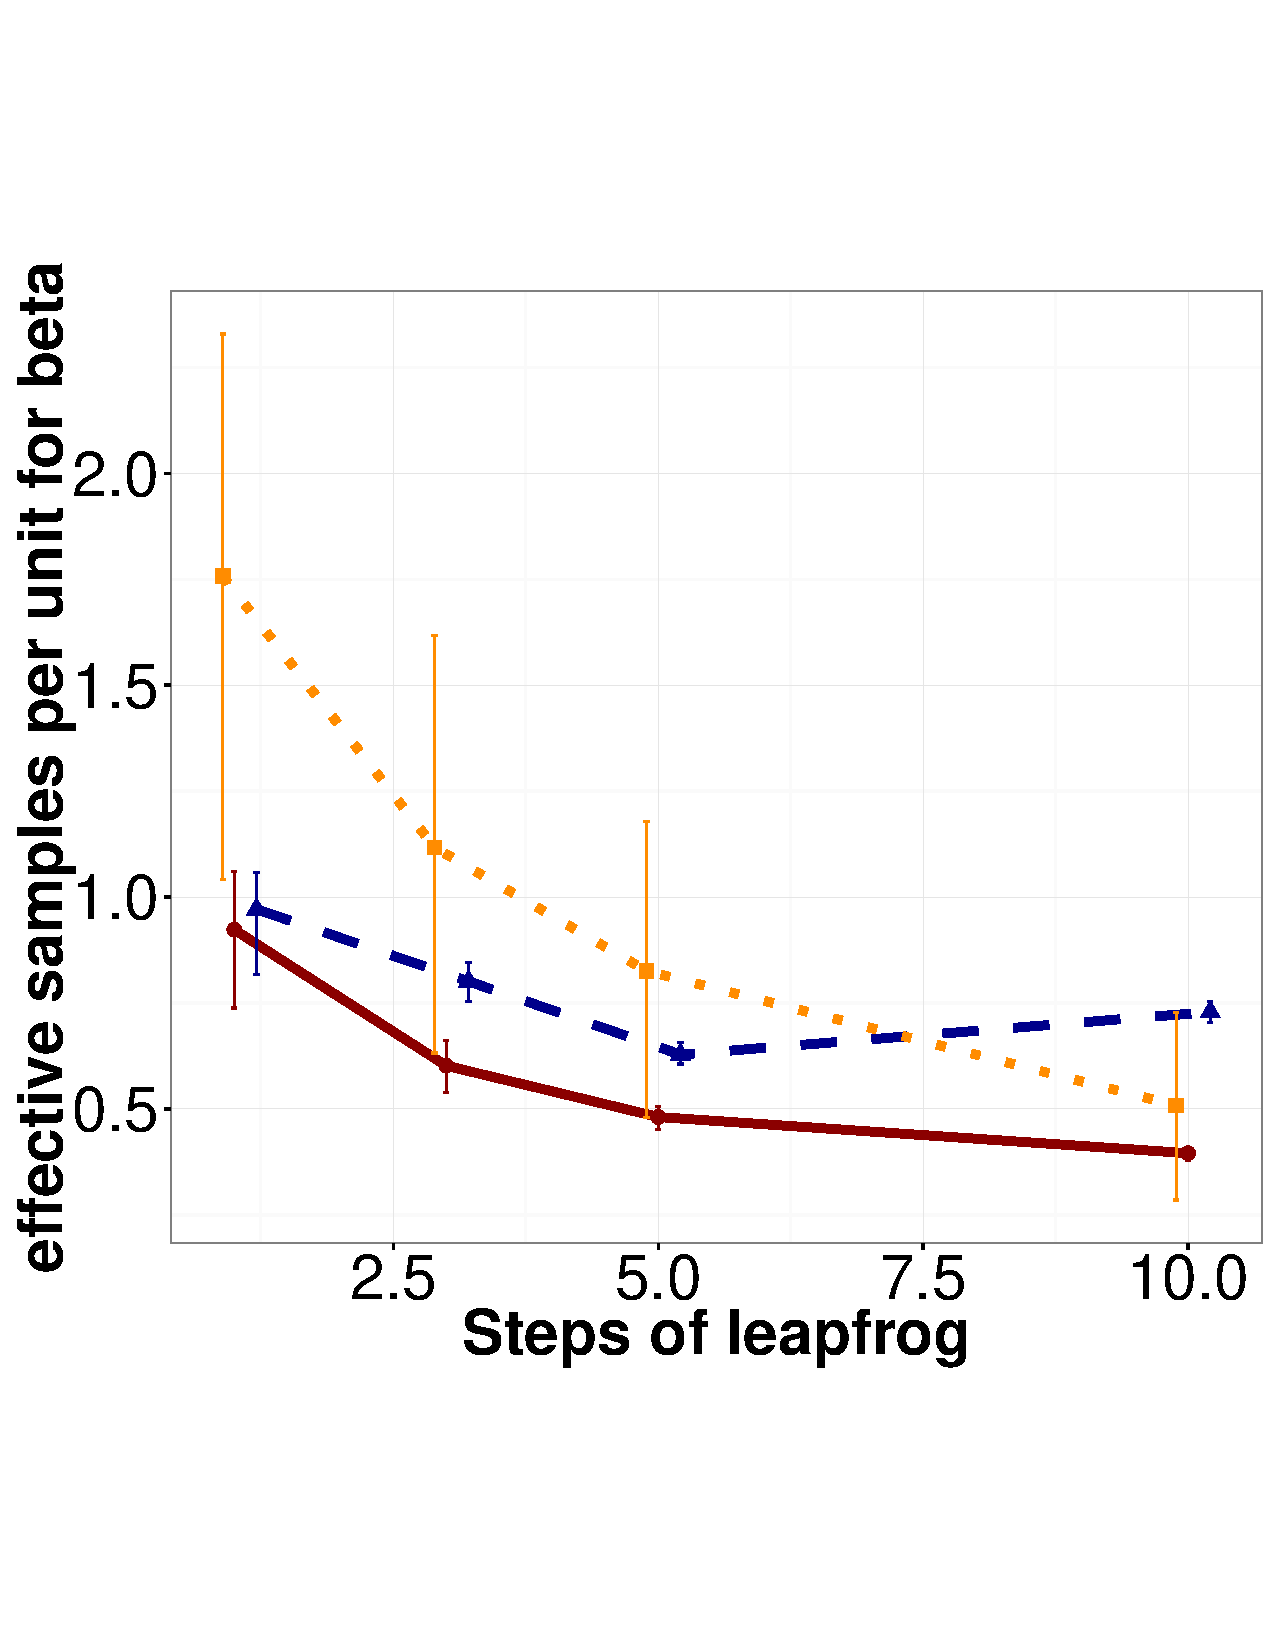
\includegraphics [width=0.70\textwidth, angle=0]{figs/h_beta.pdf}
      \end{minipage}

    \caption{HMC for dim 3}
  \end{figure}


  \begin{figure}%[b]
  \centering
  \begin{minipage}[hp]{0.45\linewidth}
  \centering
    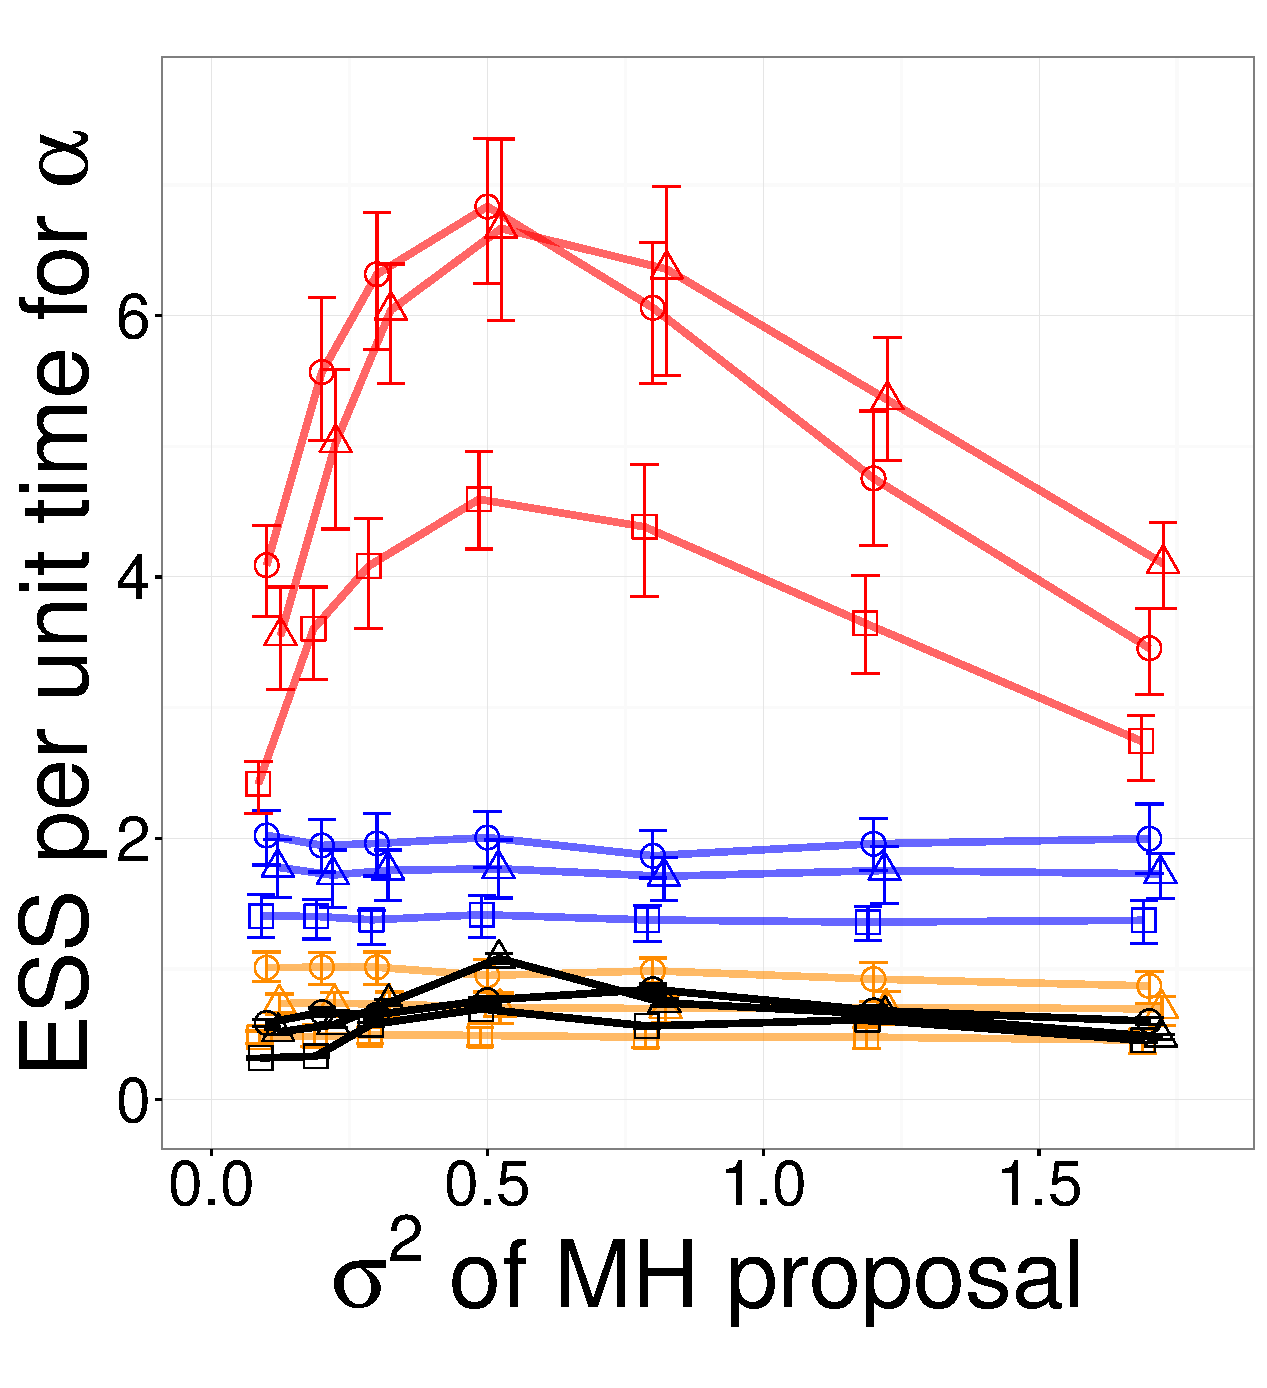
\includegraphics [width=0.70\textwidth, angle=0]{figs/exp_5_alpha.pdf}
%    \caption{ESS/sec for exp model (alpha, dim 5)}
      \end{minipage}
  \begin{minipage}[hp]{0.45\linewidth}
  \centering
    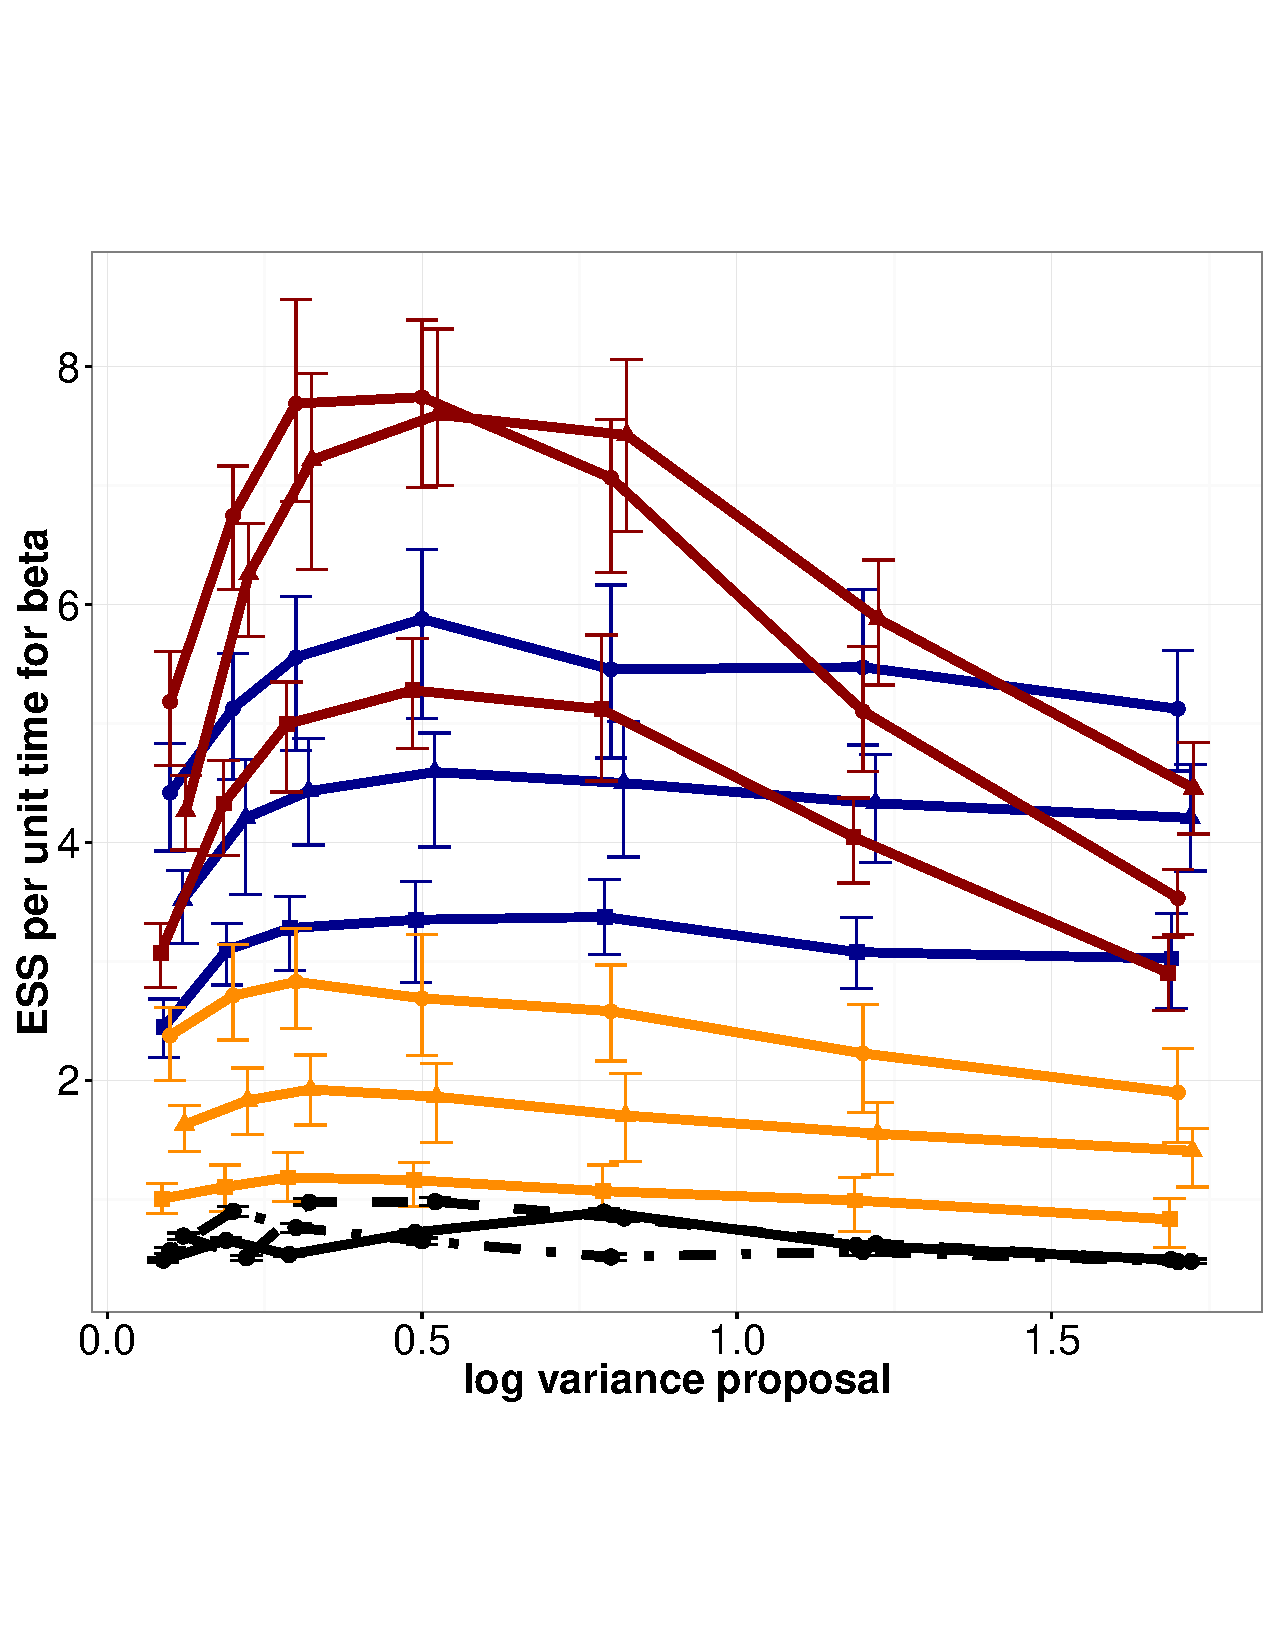
\includegraphics [width=0.70\textwidth, angle=0]{figs/exp_5_beta.pdf}
    \vspace{-0 in}
%    \caption{ESS/sec for exp model (beta, dim 5)}
     \label{fig:ESS_EXP_D5}
  \end{minipage}
    \caption{ESS/sec for exp model (dim 5)}
  \end{figure}

  \begin{figure}%[b]
  \centering
  \begin{minipage}[hp]{0.45\linewidth}
  \centering
    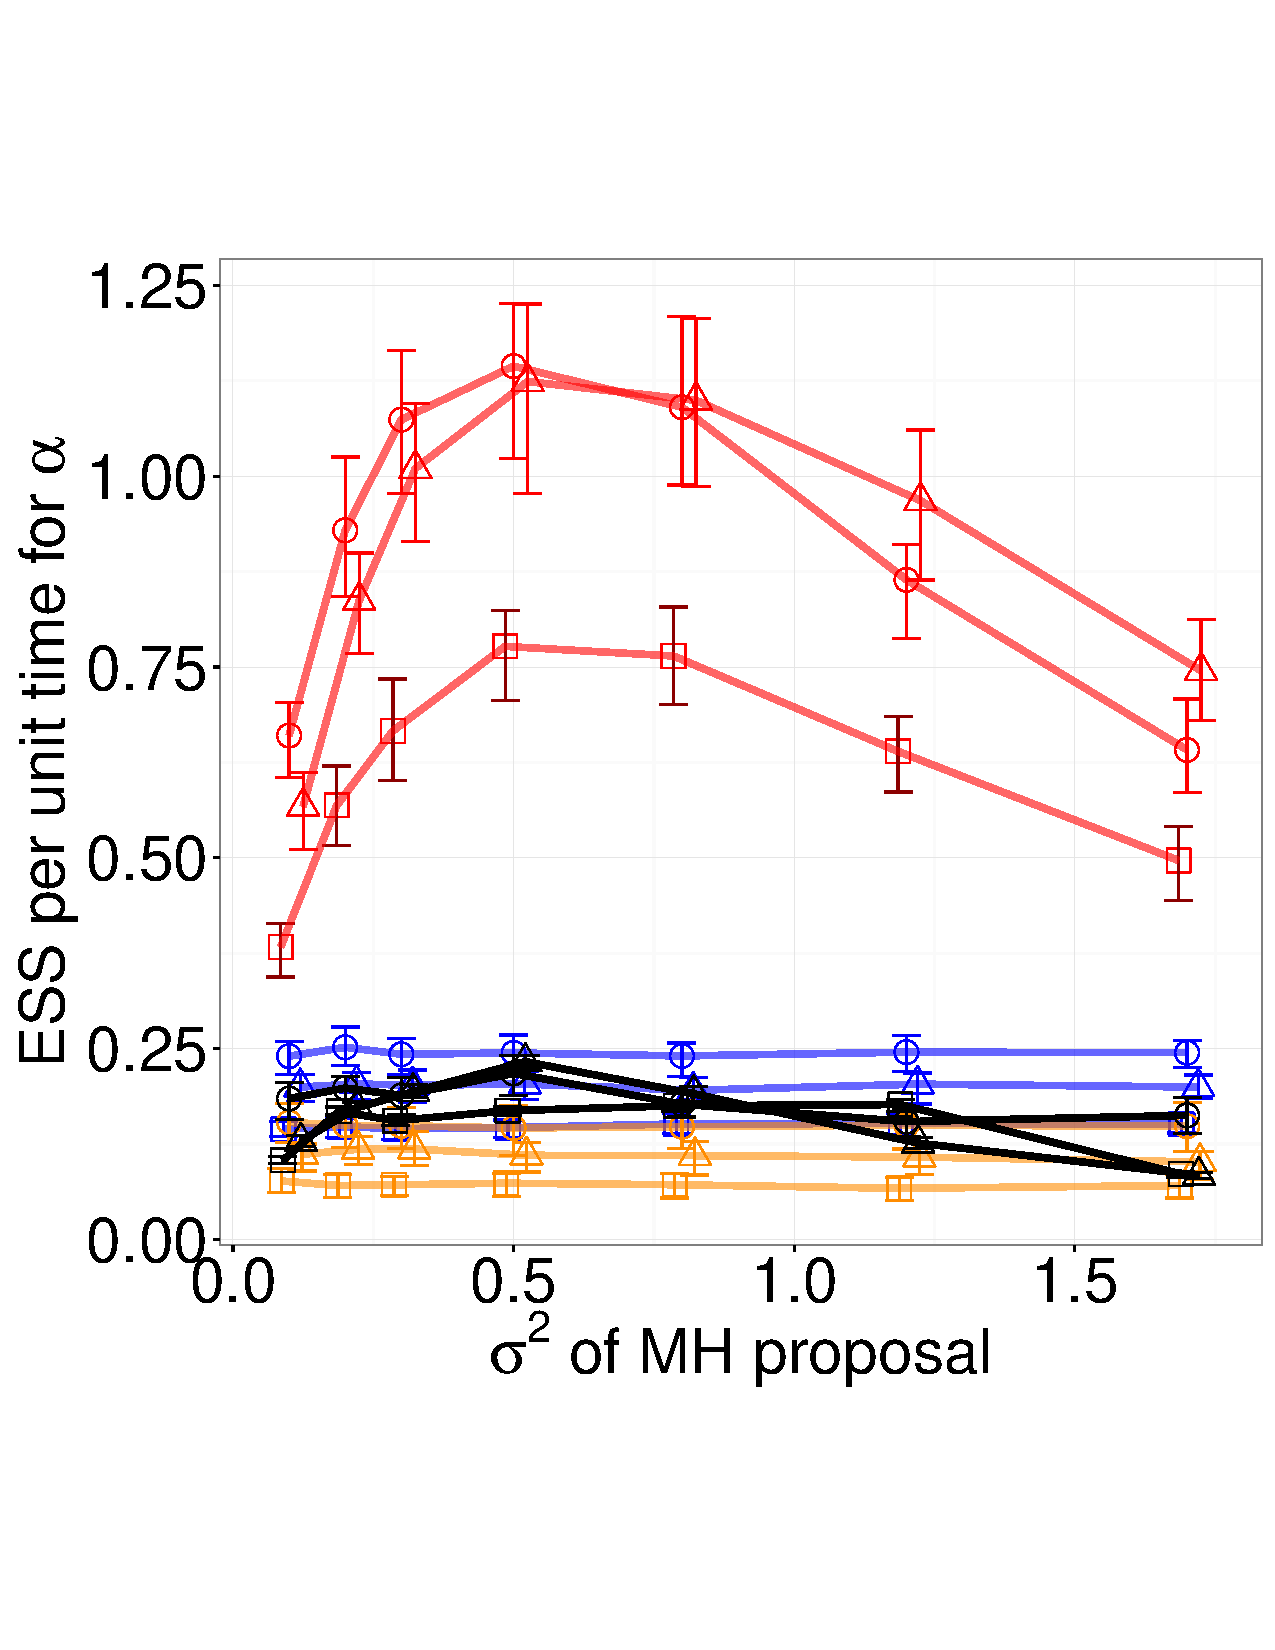
\includegraphics [width=0.70\textwidth, angle=0]{figs/exp_10_alpha.pdf}
      \end{minipage}
  \begin{minipage}[!hp]{0.45\linewidth}
  \centering
    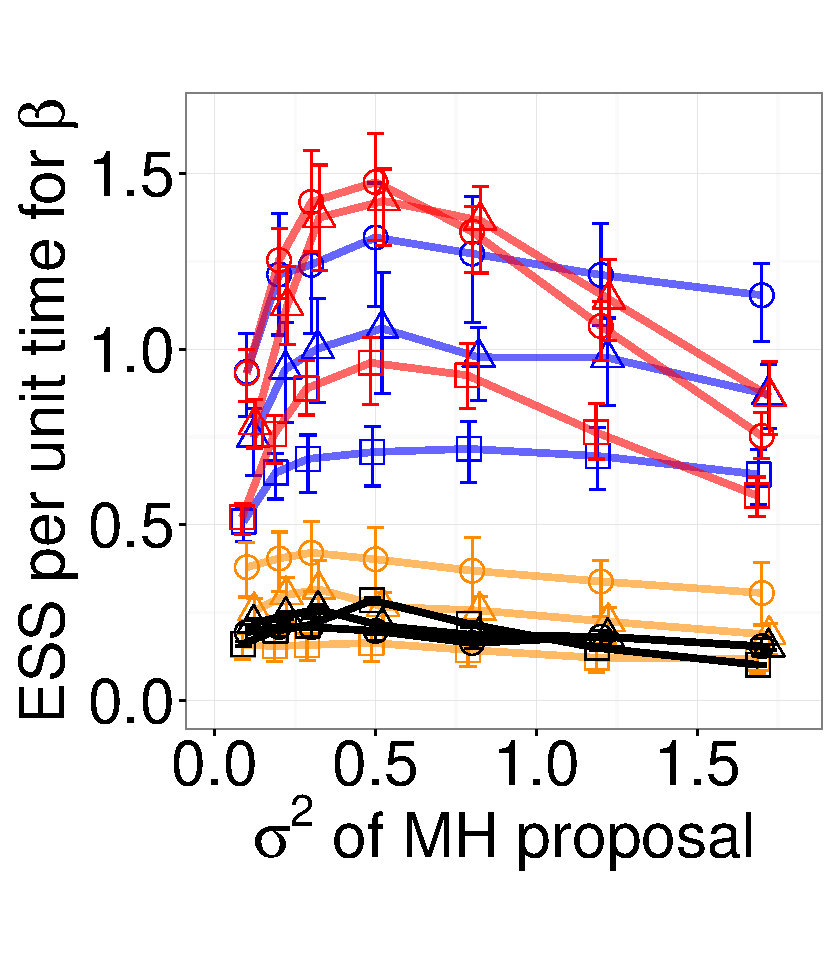
\includegraphics [width=0.70\textwidth, angle=0]{figs/exp_10_beta.pdf}
    \vspace{-0 in}
     \label{fig:ESS_EXP_D10}
  \end{minipage}
    \caption{ESS/sec for exp model (dim 10)}
  \end{figure}
  
  
  
  \begin{figure}%[b]
  \centering
  \begin{minipage}[hp]{0.45\linewidth}
  \centering
    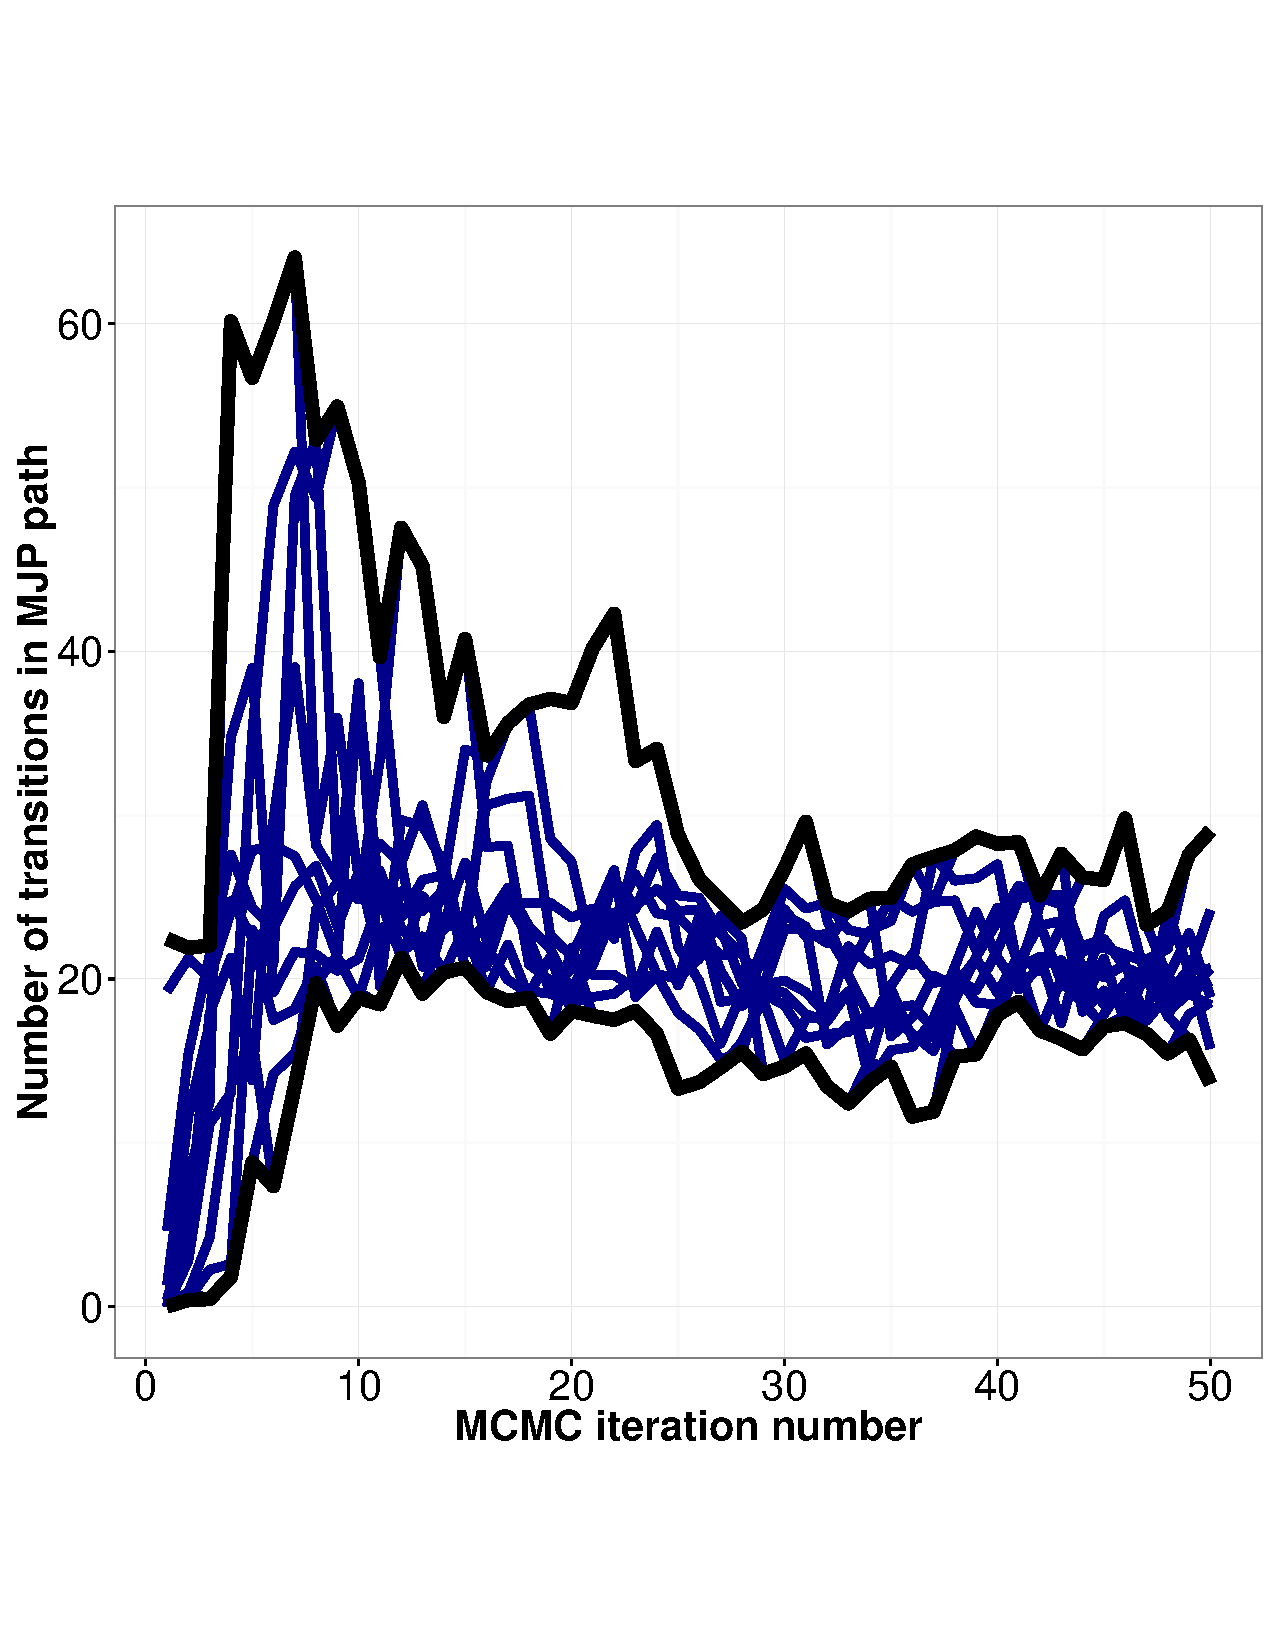
\includegraphics [width=0.70\textwidth, angle=0]{figs/exp3_k2_path_transition.pdf}
    \caption{Trace plot of the number of MJP transitions for different initializatoins for exponential model.}
      \end{minipage}
  \end{figure}

  \begin{figure}%[b]
  \centering
  \begin{minipage}[hp]{0.45\linewidth}
  \centering
    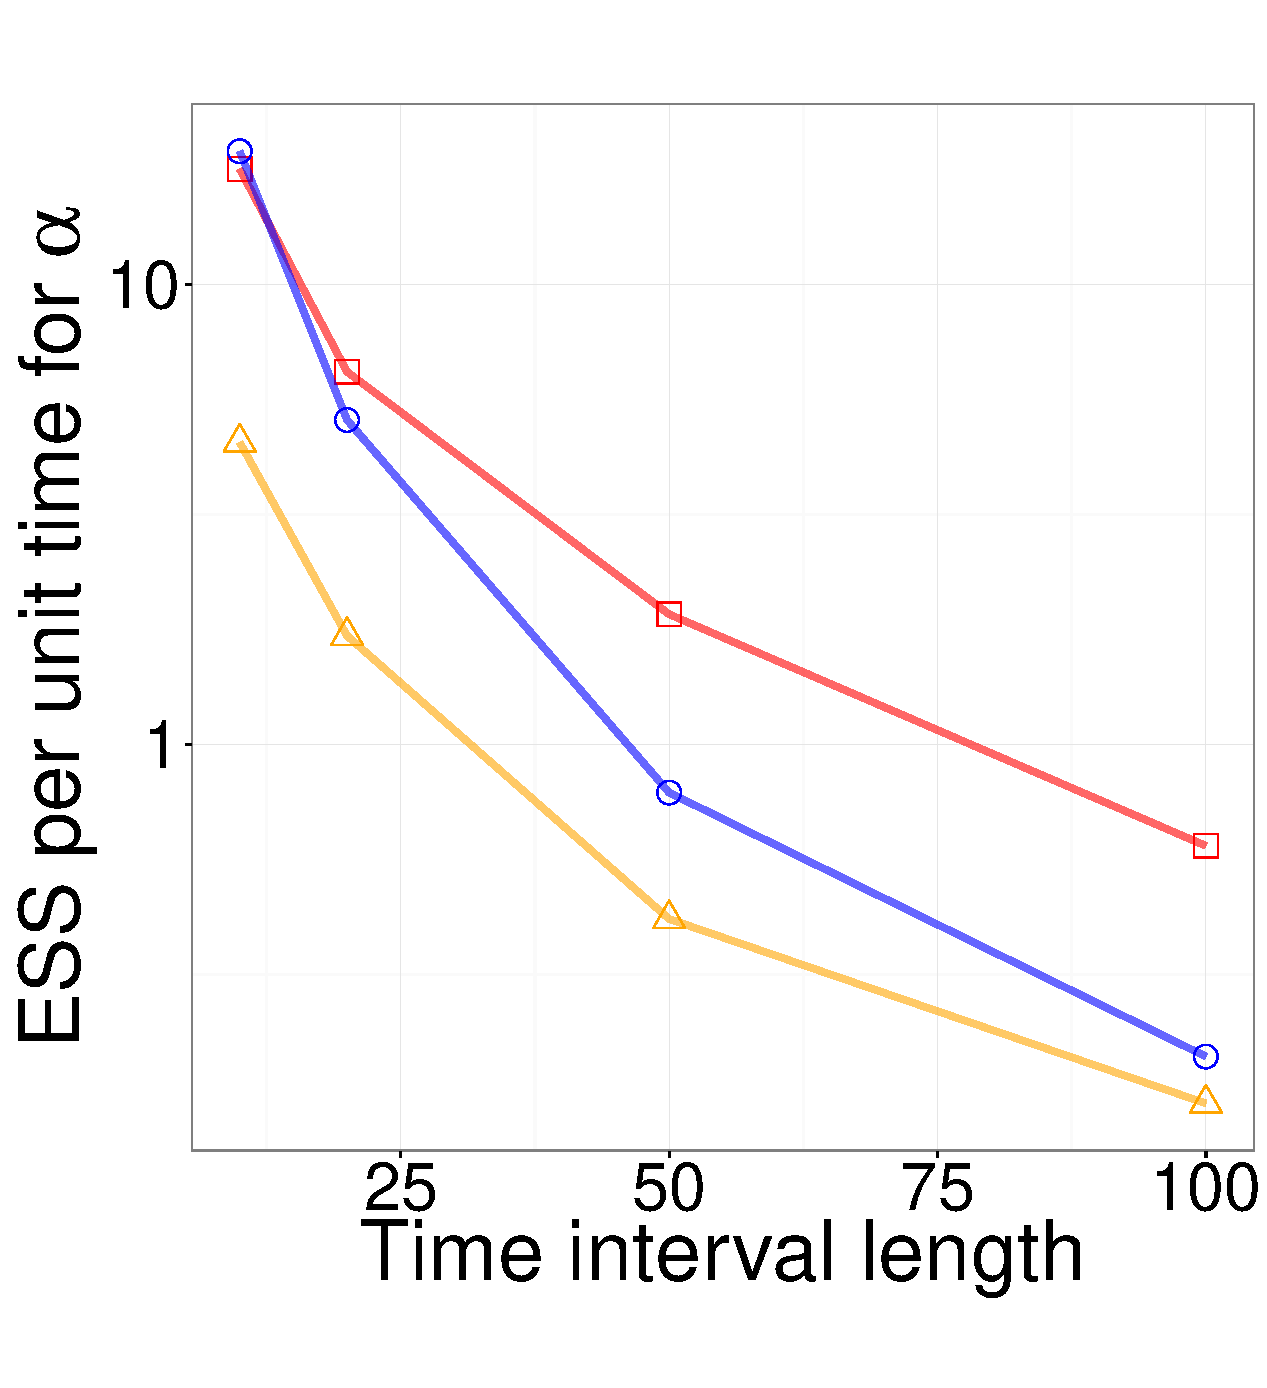
\includegraphics [width=0.70\textwidth, angle=0]{figs/ESS_vs_t_alpha.pdf}
      \end{minipage}
  \begin{minipage}[hp]{0.45\linewidth}
  \centering
    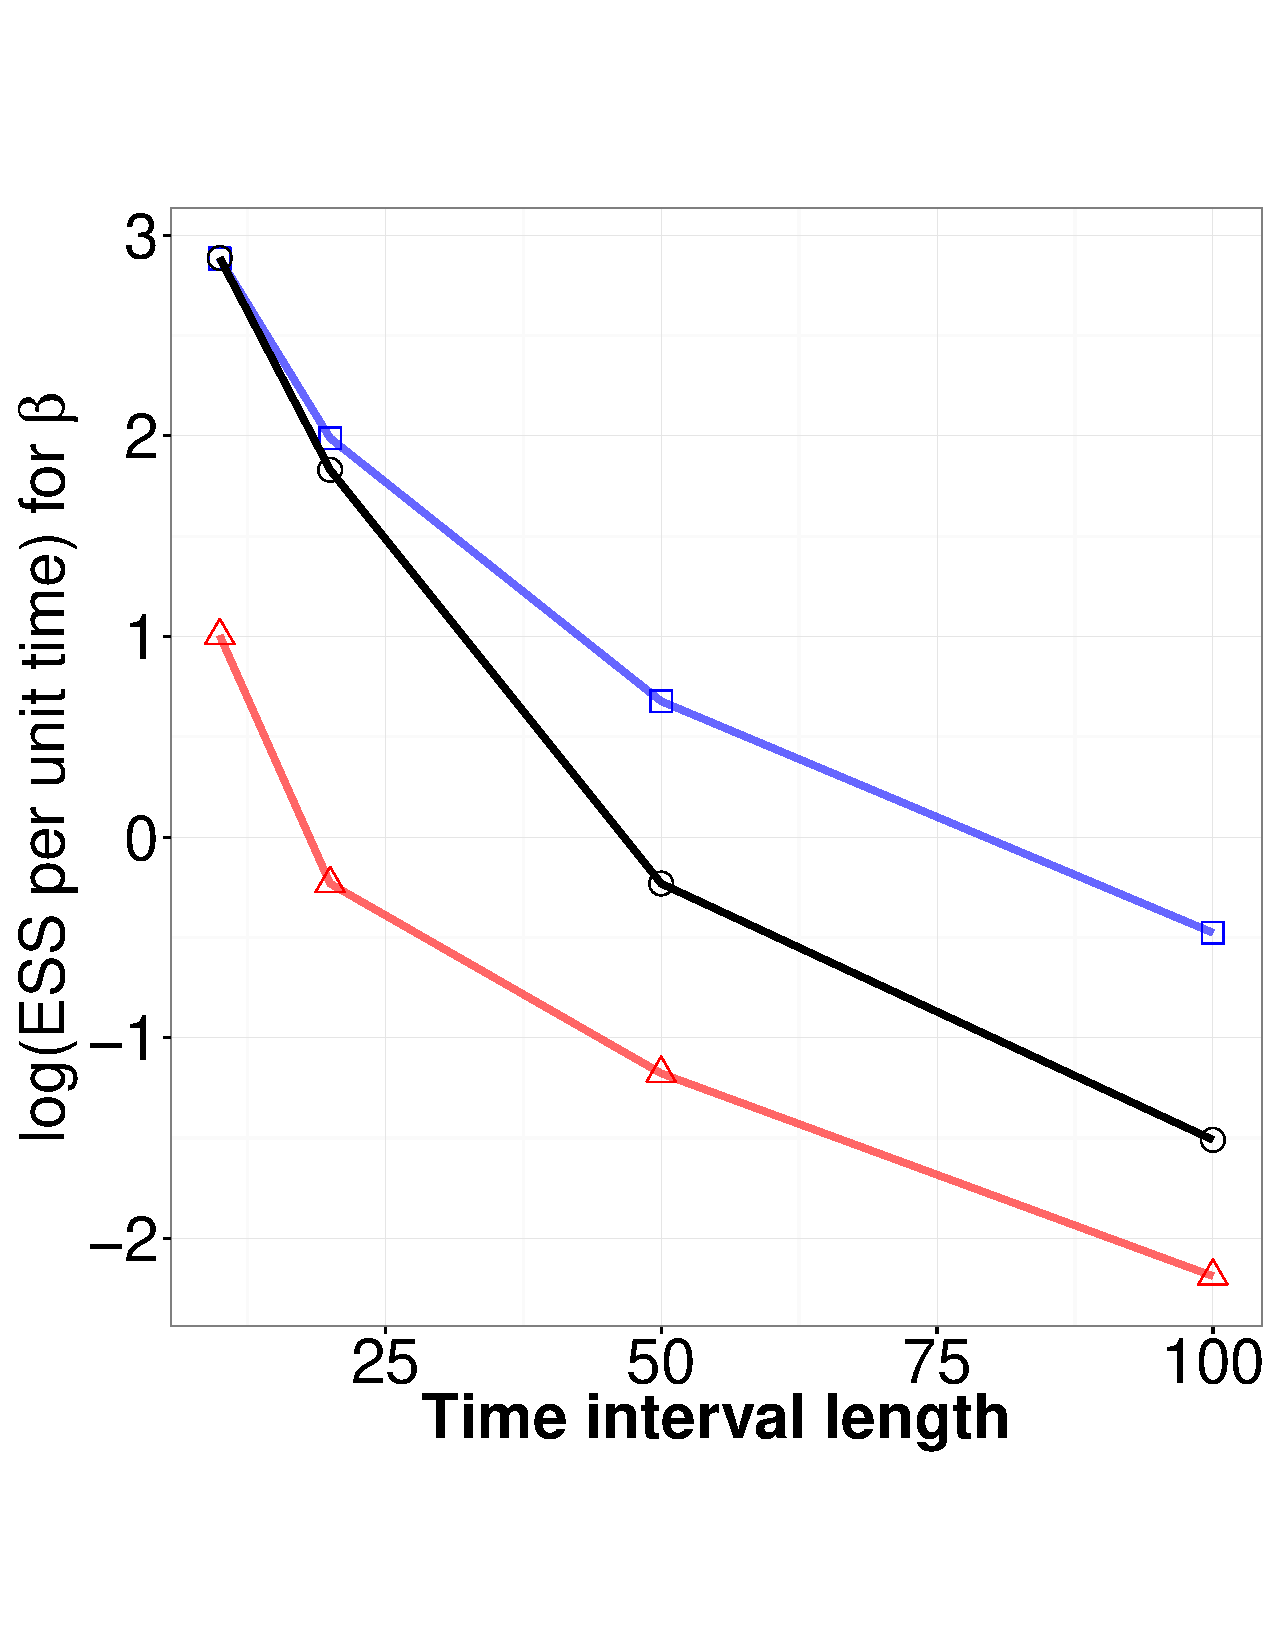
\includegraphics [width=0.70\textwidth, angle=0]{figs/ESS_vs_t_beta.pdf}
    \vspace{-0 in}
     \label{fig:TSS}
  \end{minipage}
    \caption{Time Interval vs. ESS / sec}
  \end{figure}

  \begin{figure}%[b]  
  \centering
  \begin{minipage}[hp]{0.45\linewidth}
  \centering
    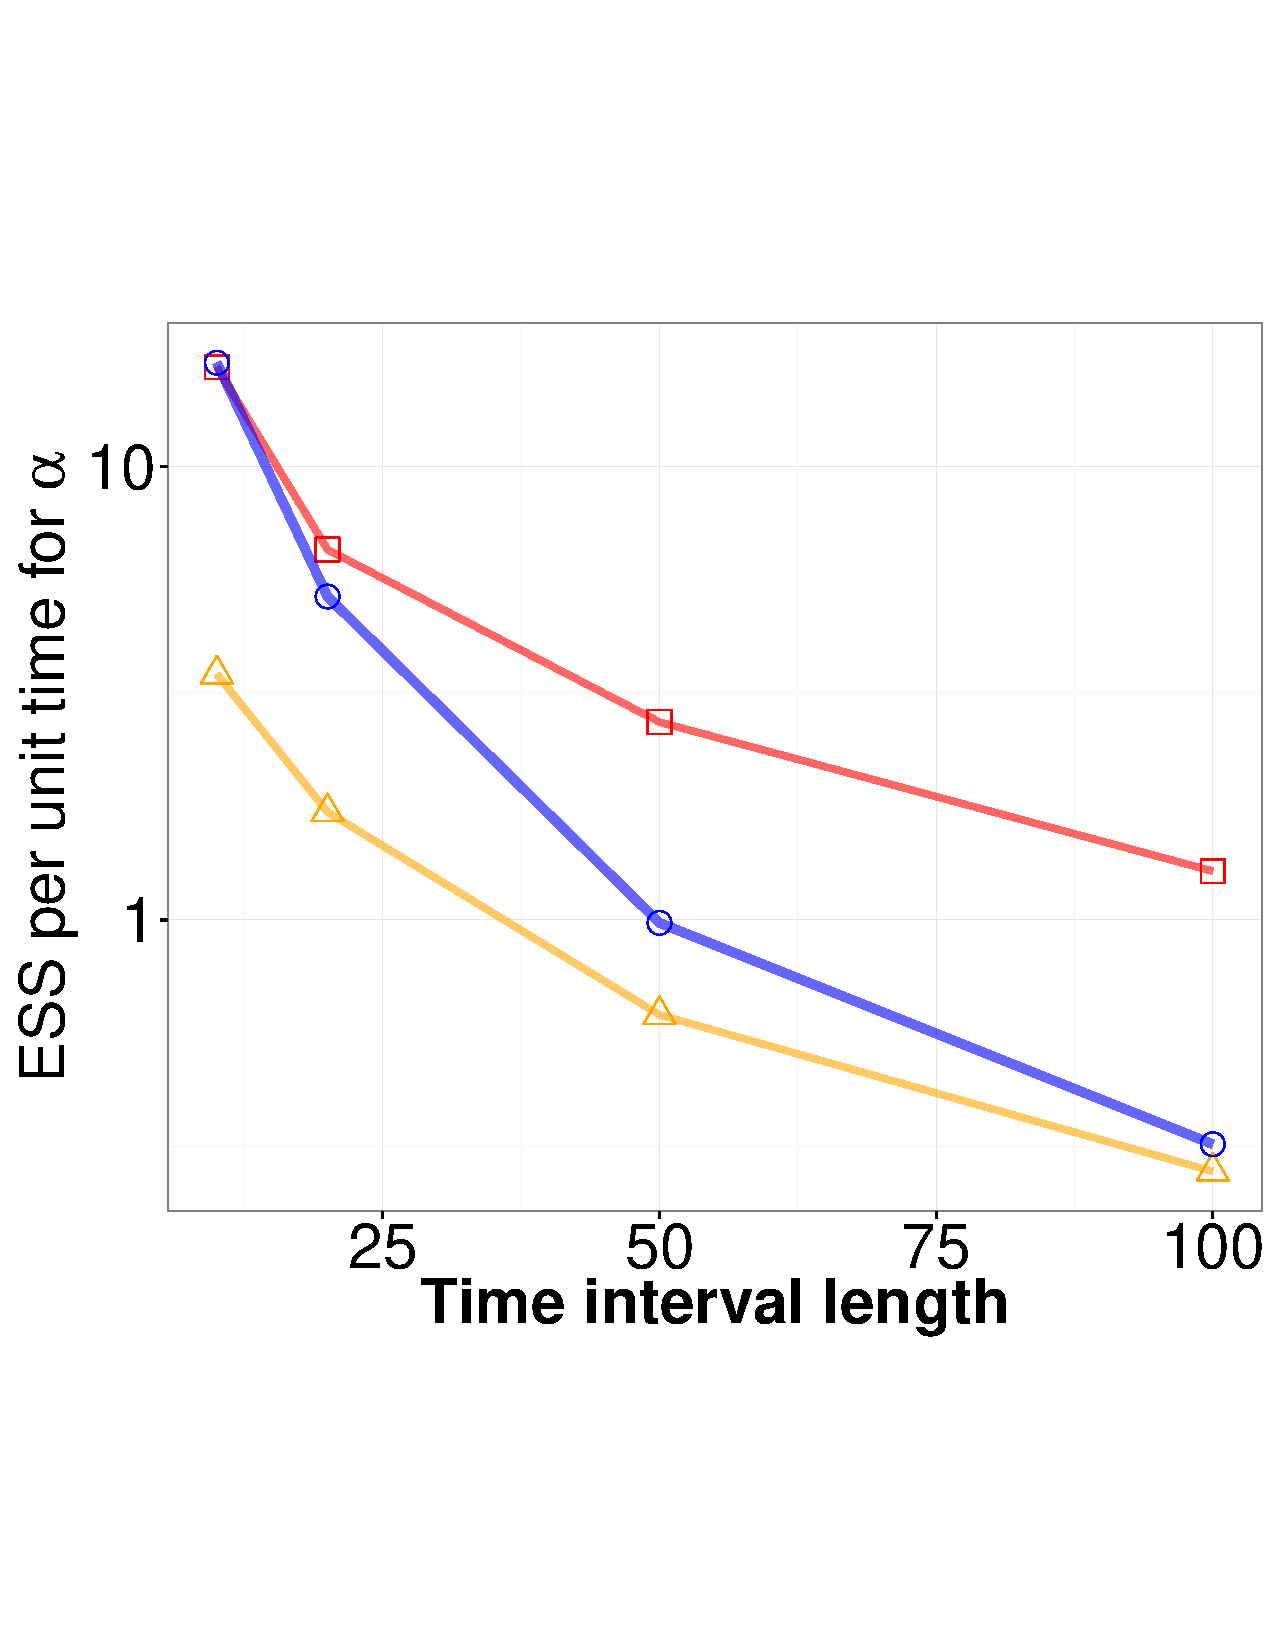
\includegraphics [width=0.70\textwidth, angle=0]{figs/ESS_vs_t_alpha_fixobservation.pdf}
    \end{minipage}
  \begin{minipage}[hp]{0.45\linewidth}
  \centering
    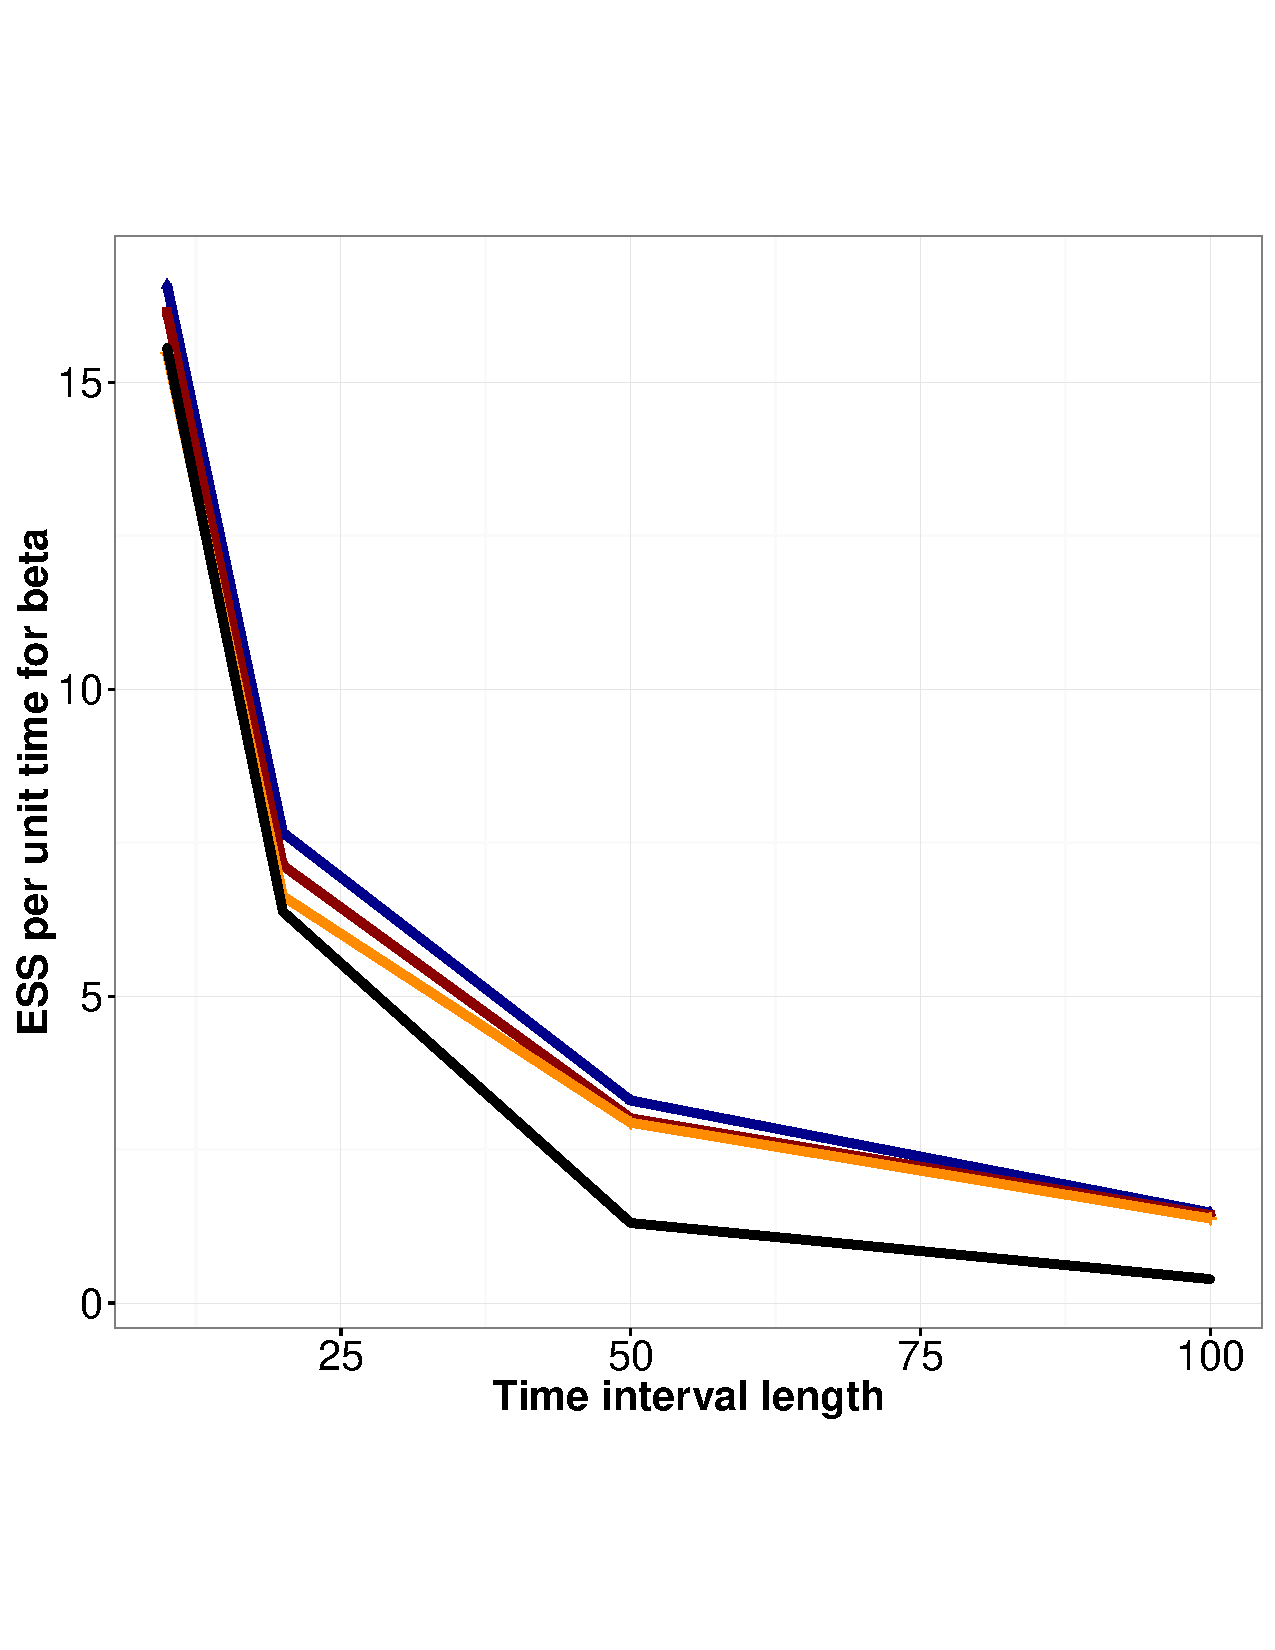
\includegraphics [width=0.70\textwidth, angle=0]{figs/ESS_vs_t_beta_fixobservation.pdf}
    \vspace{-0 in}
     \label{fig:TSS2}
  \end{minipage}
    \caption{Time Interval vs. ESS / sec (Number of observations is fixed)}
  \end{figure}
  \begin{figure}%[b]
  \centering
  \begin{minipage}[hp]{0.45\linewidth}
  \centering
    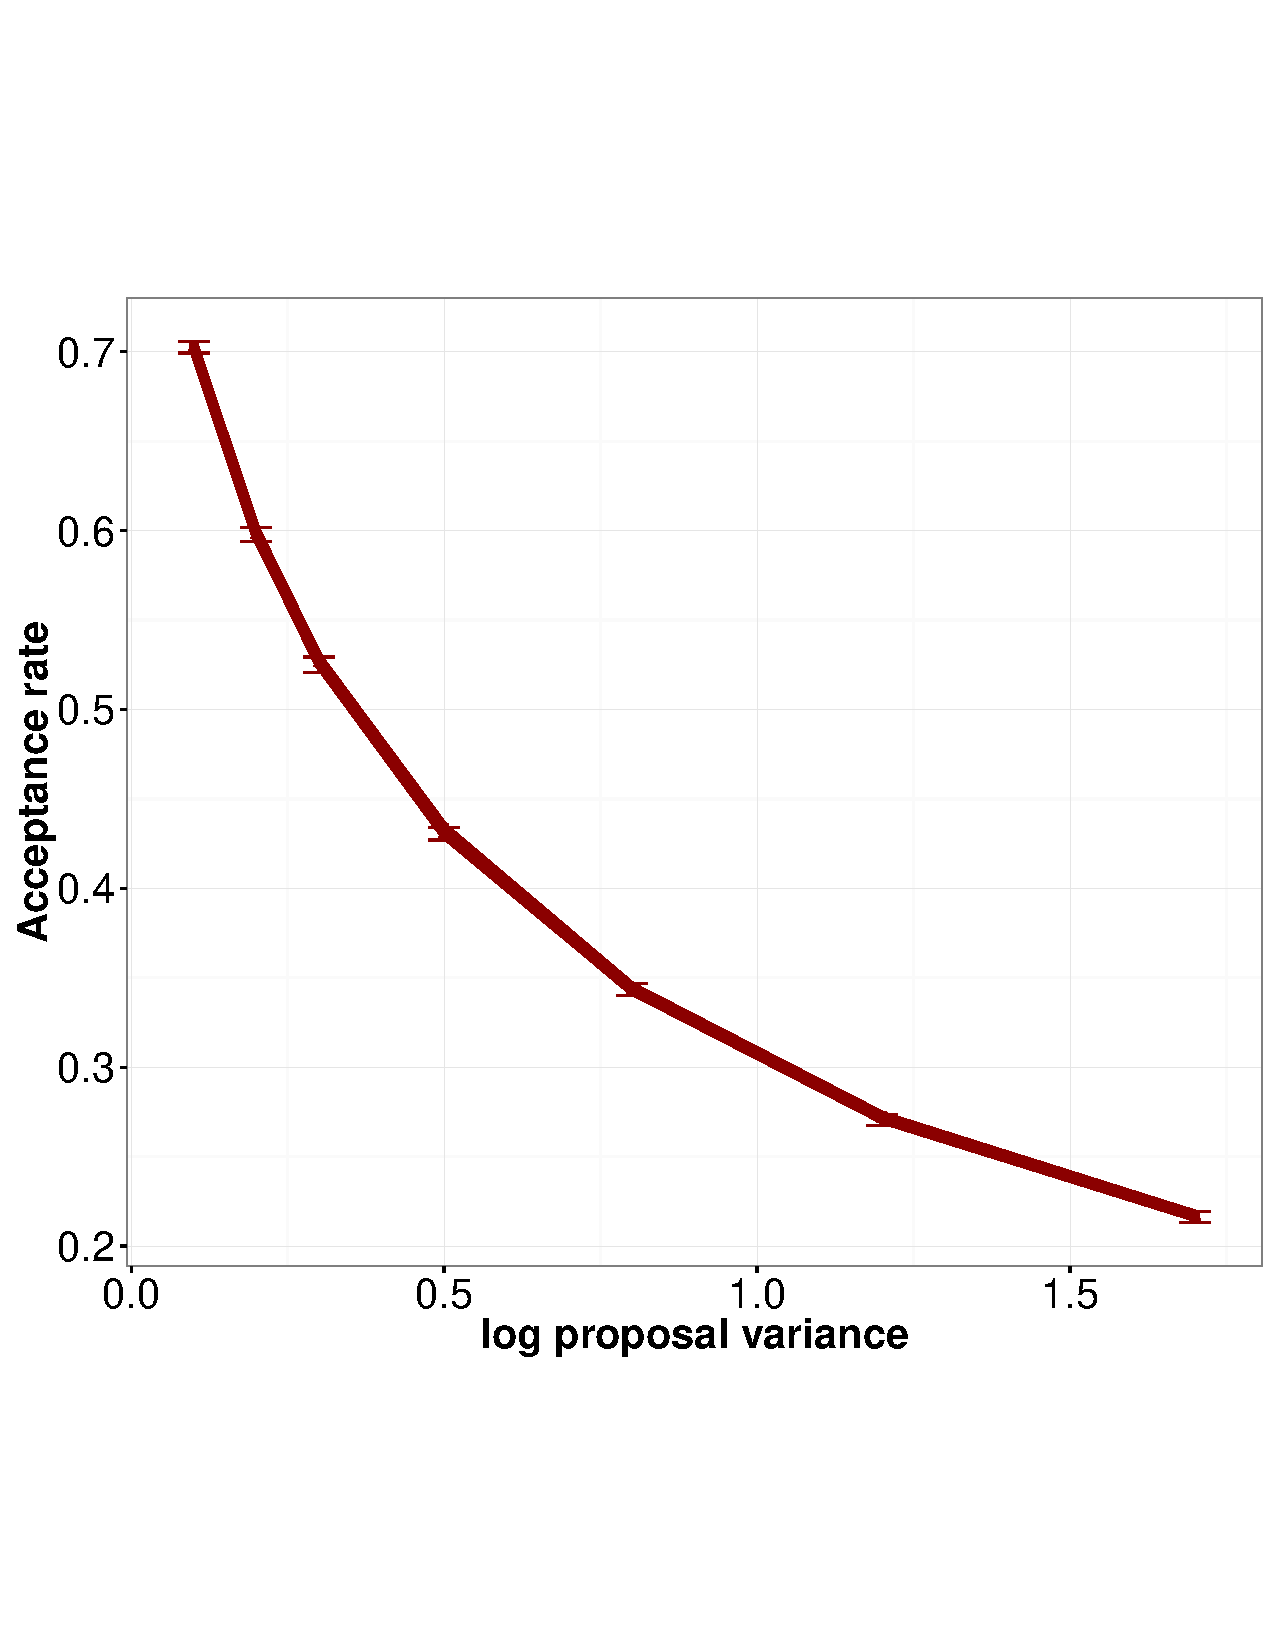
\includegraphics [width=0.70\textwidth, angle=0]{figs/acc_rate_exp_d3.pdf}
    \caption{Acceptance rate for exp model (dim 3)}
      \end{minipage}
  \end{figure}


\section{Immigration models with capacity}~
An $M/M/N/N$ queue is a stochastic process whose state space is the set $\{0, 1, 2, 3, ..., N - 1\}$ where the value corresponds to the number of customers in the system, including any currently in service. Arrivals occur at rate $\alpha$ according to a Poisson process and move the process from state $i$ to $i+1$. Service times have an exponential distribution with parameter $\beta$ in the $M/M/N/N$ queue. There are $N$ servers, which serve from the front of the queue. If there are less than $N$ jobs, some of the servers will be idle. Only $N$ customers can queue at any one time. Any further arrivals to the queue are considered "lost". 
  \begin{figure}[H]
  \centering
  \begin{minipage}[!hp]{0.6\linewidth}%0.45
  \centering
    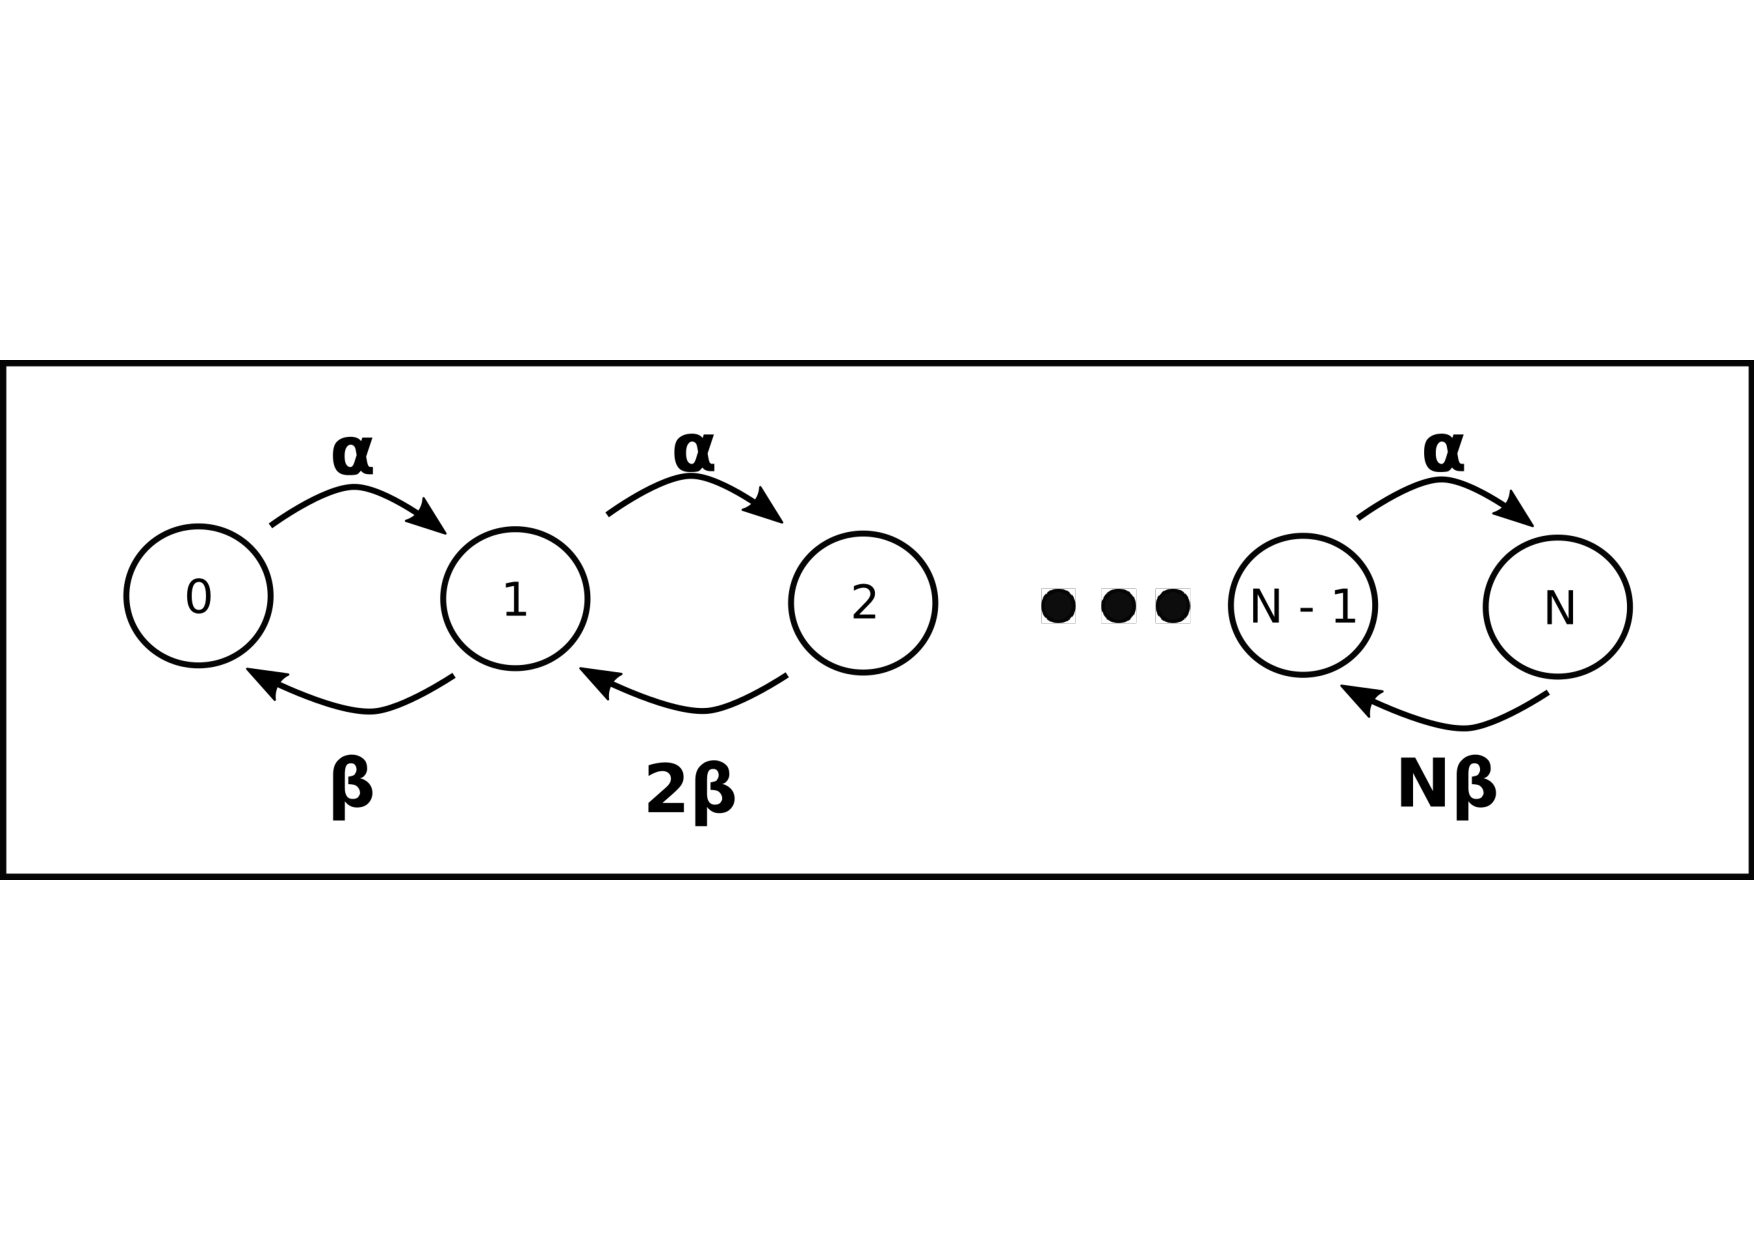
\includegraphics [width=1\textwidth, angle=0]{figs/queue_model.pdf}%0.70
      \end{minipage}
    \caption{exp model}
  \end{figure}

\noindent Assume: $S = [S_0,S_1, ...,S_N] \;, T = [t_0(t_{start}), t_1,...,t_N, t_{N+1}(t_{end})]$, and y as observations.\\
Now, let's consider a immigration model as follows. State space is $\{0, 1, 2, ..., N - 1\}$, representing the total population. The transition matrix is defined as follows. 
$$A_i =: A_{i,i} = -(\alpha + i\beta), \; \; i =0,1,...,N$$ $$A_{i, i+1} = \alpha, \; \; i =0,1,...,N-1,$$ $$A_{i, i-1}  = \beta, \; \;  i =1,...,N.$$
We already know the conditional density(given $\alpha,\; \beta$) of a MJP trajectory $(s_0, S, T)$ in time interval $[t_{start}, t_{end}]$, with $S=(s_1, s_2,..., s_k)$, $T=(t_1, t_2,..., t_k)$. 
$$f(s_0,S,T| \alpha, \beta) = \prod_{i=0}^{k-1} A_{s_i, s_{i+1}} \exp(\sum_{i=0}^{k} A_{s_i}(t_{i+1} - t_{i})), $$
where $t_0 = t_{start}$, $t_{k+1} = t_{end}.$\\
Let's denote some notations here.\\
$$U(s_0, S, T):= \sum_{i=0}^{k-1} \mathbb{I}_{\{s_{i+1} - s_i = 1\}}.$$
$$D(s_0, S, T):= \sum_{i=0}^{k-1} \mathbb{I}_{\{s_{i+1} - s_i = -1\}}.$$
Call them U and D for short.
Let's denote the total time when the trajectory state stays at state i as $\tau_i$, i.e. $\tau_i = \sum_{j=0}^{k} (t_{j+1} -t_j)\mathbb{I}_{\{s_j = i\}}$, then $\sum_{i=0}^k (t_{i+1} - t_i)s_i = \sum_{i=0}^N \tau_ii.$\\

$$f(s_0,S,T| \alpha, \beta) = \exp(-\alpha(t_{end} - t_{start}- \tau_N) )\alpha^U \cdot  \exp((-(\sum_{i=0}^k (t_{i+1} - t_i)s_i)\beta) \prod_{i=1}^N i^{\sum_{j=0}^{k-1}\mathbb{I}_{s_{j+1} = i -1 \;,  s_j = i} }   \beta^D$$\\
If we assume the prior of $\alpha$, and $\beta$ are $Gamma(\mu,\lambda)$, $Gamma(\omega, \theta)$, which are independent with each other. \\
$$p(\alpha) = \frac{\lambda^\mu}{\Gamma(\mu)}\alpha^{\mu -1}e^{-\lambda \alpha}. $$
$$p(\beta) = \frac{\theta^\omega}{\Gamma(\omega)}\beta^{\omega -1}e^{-\theta \beta}. $$
Then we can get the posterior distribution $$f(\alpha, \beta | s_0,S,T)$$ as follows.
$$ f(\alpha, \beta | s_0,S,T) \propto \exp(-(\lambda + t_{end} - t_{start}- \tau_N)\alpha) \alpha^{\mu + U -1} \cdot \exp(-(\sum_{i=0}^k (t_{i+1} - t_i)s_i + \theta)\beta) \beta^{\omega+ D -1}.$$
It means that the posterior distributions of $\alpha$, $\beta$ are still independent. \\
$\alpha | s_0,S,T$ is following $Gamma(\mu+ U,\lambda + t_{end} - t_{start}- \tau_N)$\\
$\beta | s_0,S,T$ is following $Gamma(\omega+ D,\theta + \sum_{i=0}^k (t_{i+1} - t_i)s_i)$, which is equivalent to $Gamma(\omega+ D,\theta +\sum_{i=0}^N \tau_ii)$\\
Such immigration models have perfectly conjugate posterior distributions when we assign $\gamma$ priors to $\alpha$ and $\beta$. We apply our Metropolis Hasting algorithms on such models to compare the performance with the performance of Gibbs Sampling algorithm.
\subsection{Experiments}
In the following, we evaluate a Python implementation of our algorithms compared to other exact samplers which include Gibbs sampler and Particle MCMC sampler. We consider three different dimensions which are 3, 5, and 10 and three different k which are 1.5, 2, and 3. We generated random parameters $\alpha$, $\beta$ from prior distributions ($Gamma(3,2), Gamma(5, 2)$), and used this to construct the transition matrix A. Then we generate an MJP trajectory with a uniform initial distribution over states. The state of this MJP trajectory was observed via a Normal distribution with mean equal to the value of state and variance 1, and posterior samples given the observations were produced by a Python implementation of our algorithm. 100 MCMC runs were performed, each run consisting of 10000(Varies among different dimensions) iterations. For each run, the number of transitions as well as the time spent was calculated, and effective sample sizes (ESSs) of these statistics (the number of independent samples with the same `information' as the correlated MCMC samples) were calculated using R-CODA (Plummer et al., 2006). The overall ESS of a run is defined to be the mean ESS across all these ESSs.

  \begin{figure}%[b]
  \centering
  \begin{minipage}[!hp]{0.45\linewidth}
  \centering
    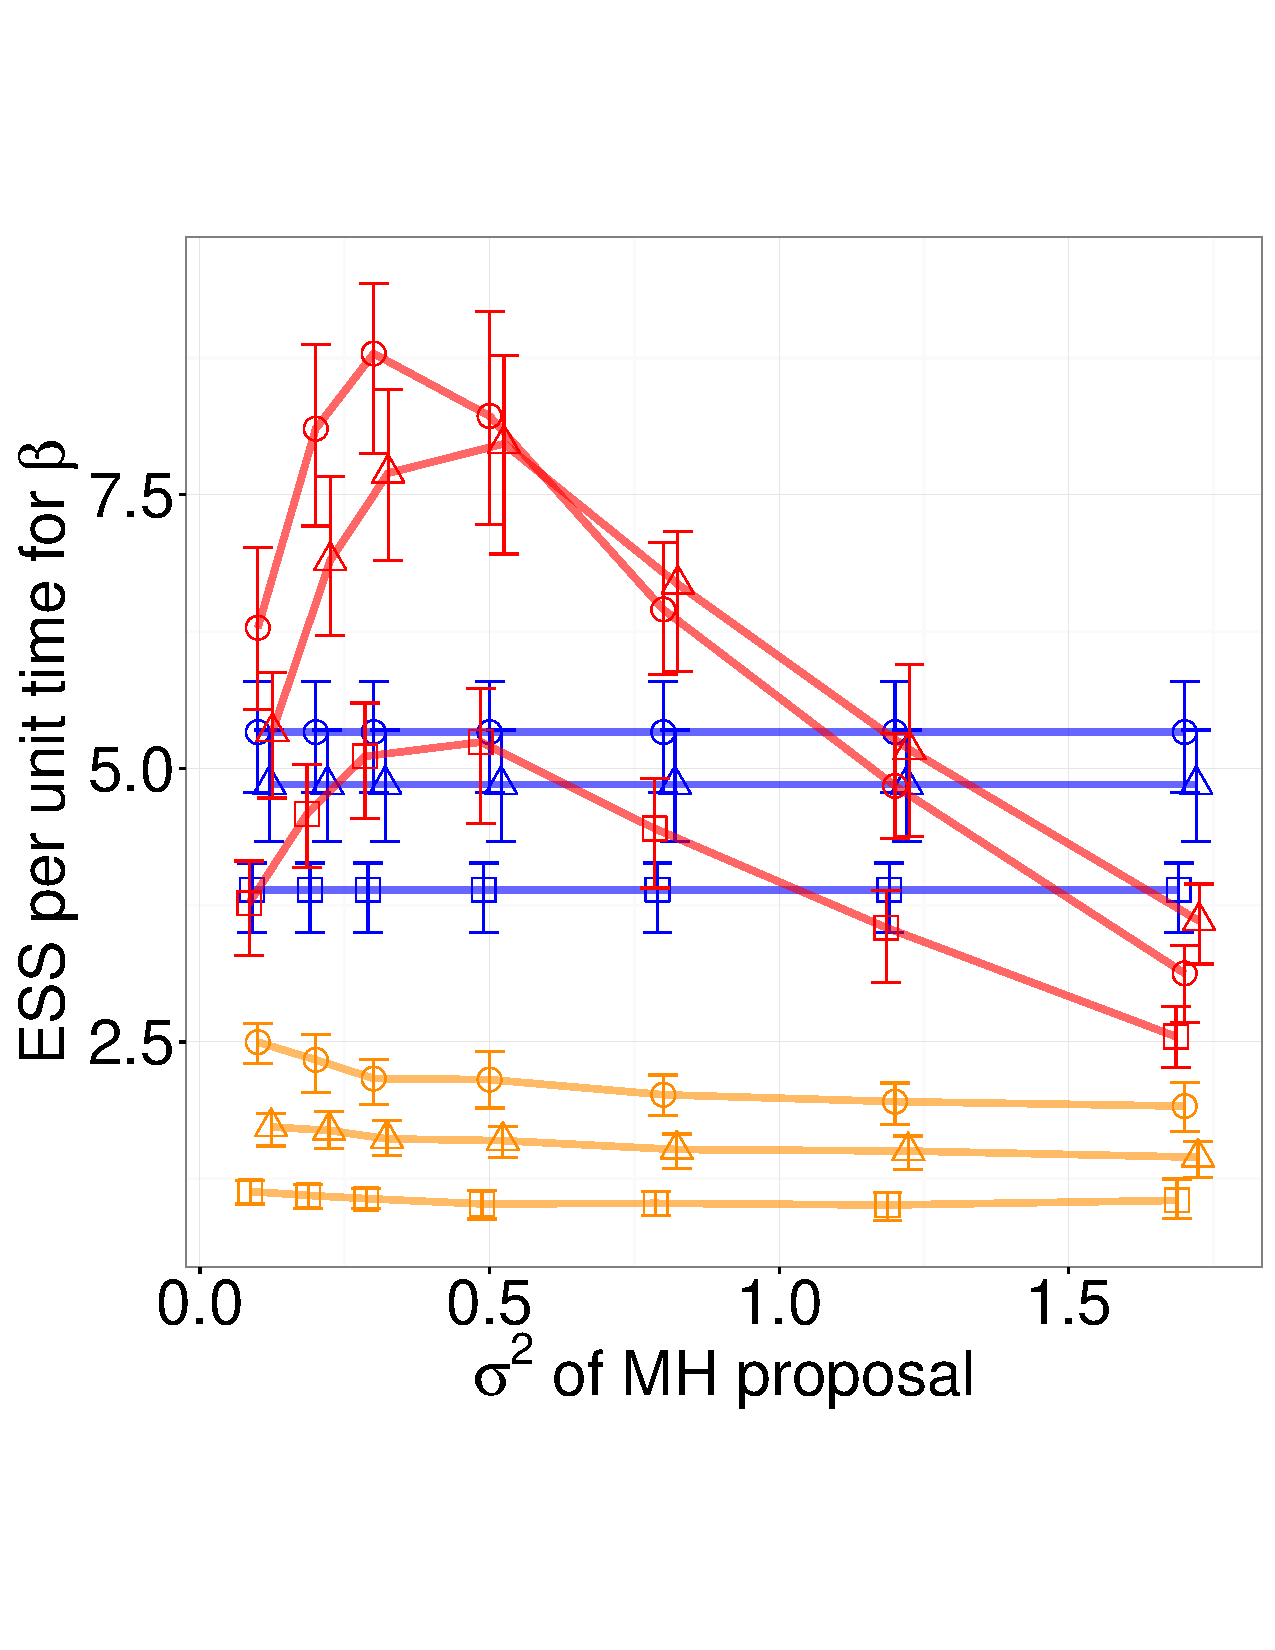
\includegraphics [width=0.70\textwidth, angle=0]{figs/q_3_alpha.pdf}
      \end{minipage}
  \begin{minipage}[!hp]{0.45\linewidth}
  \centering
    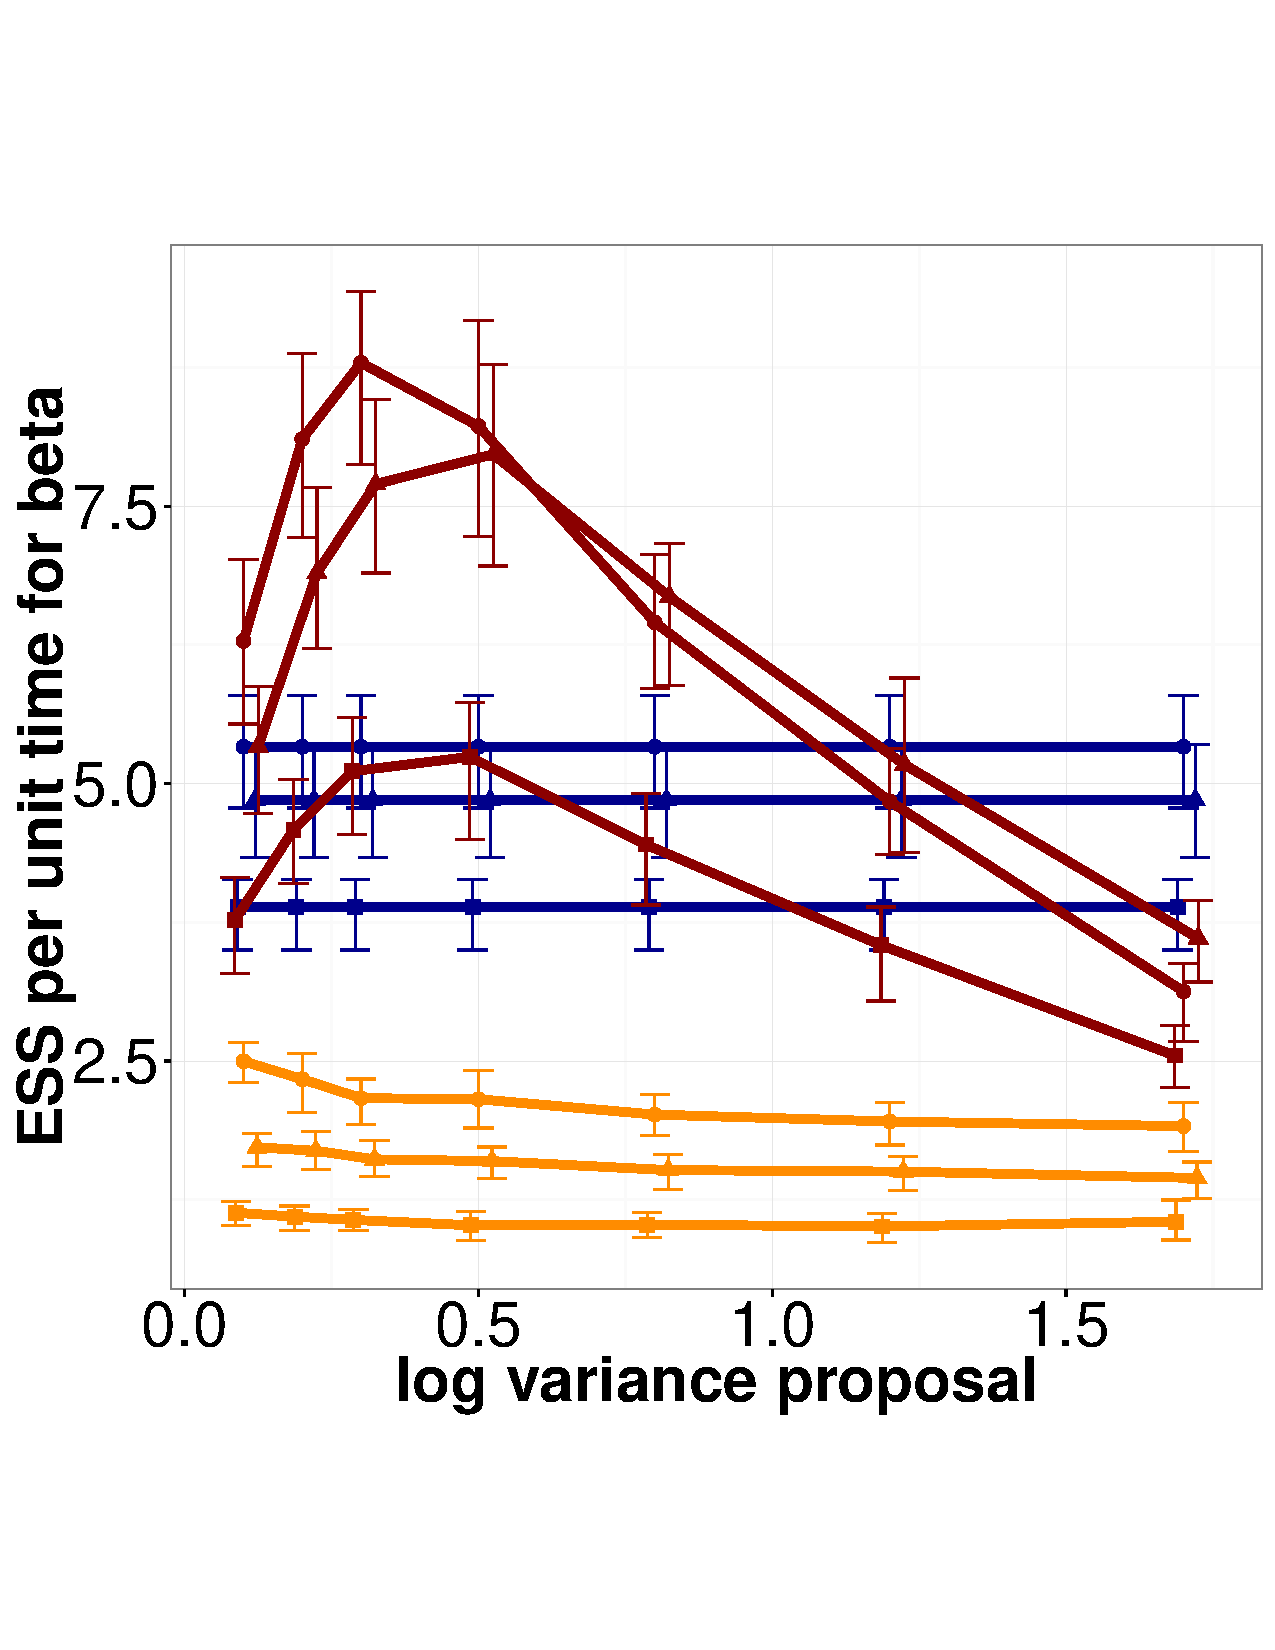
\includegraphics [width=0.70\textwidth, angle=0]{figs/q_3_beta.pdf}
    \vspace{-0 in}
     \label{fig:ESS_Q_3}
  \end{minipage}
    \caption{ESS/sec for Immigration model (dim 3)}
  \end{figure}
  \begin{figure}%[b]
  \centering
  \begin{minipage}[!hp]{0.45\linewidth}
  \centering
    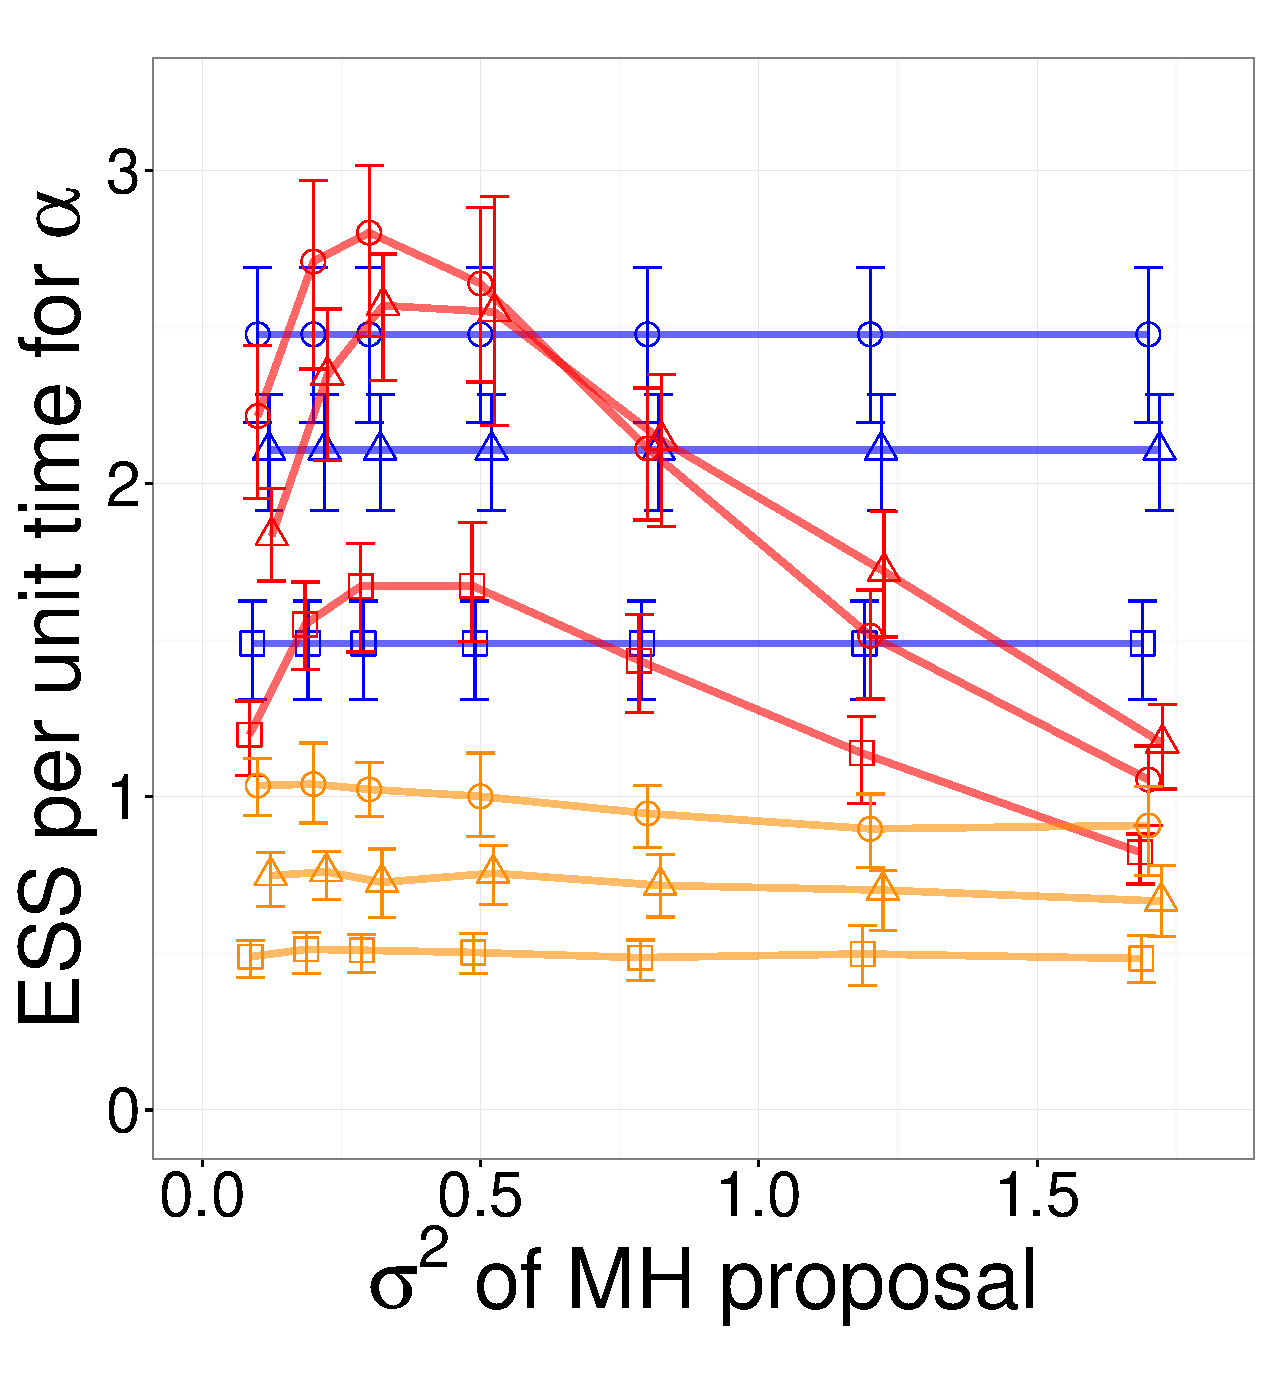
\includegraphics [width=0.70\textwidth, angle=0]{figs/q_5_alpha.pdf}
      \end{minipage}
  \begin{minipage}[!hp]{0.45\linewidth}
  \centering
    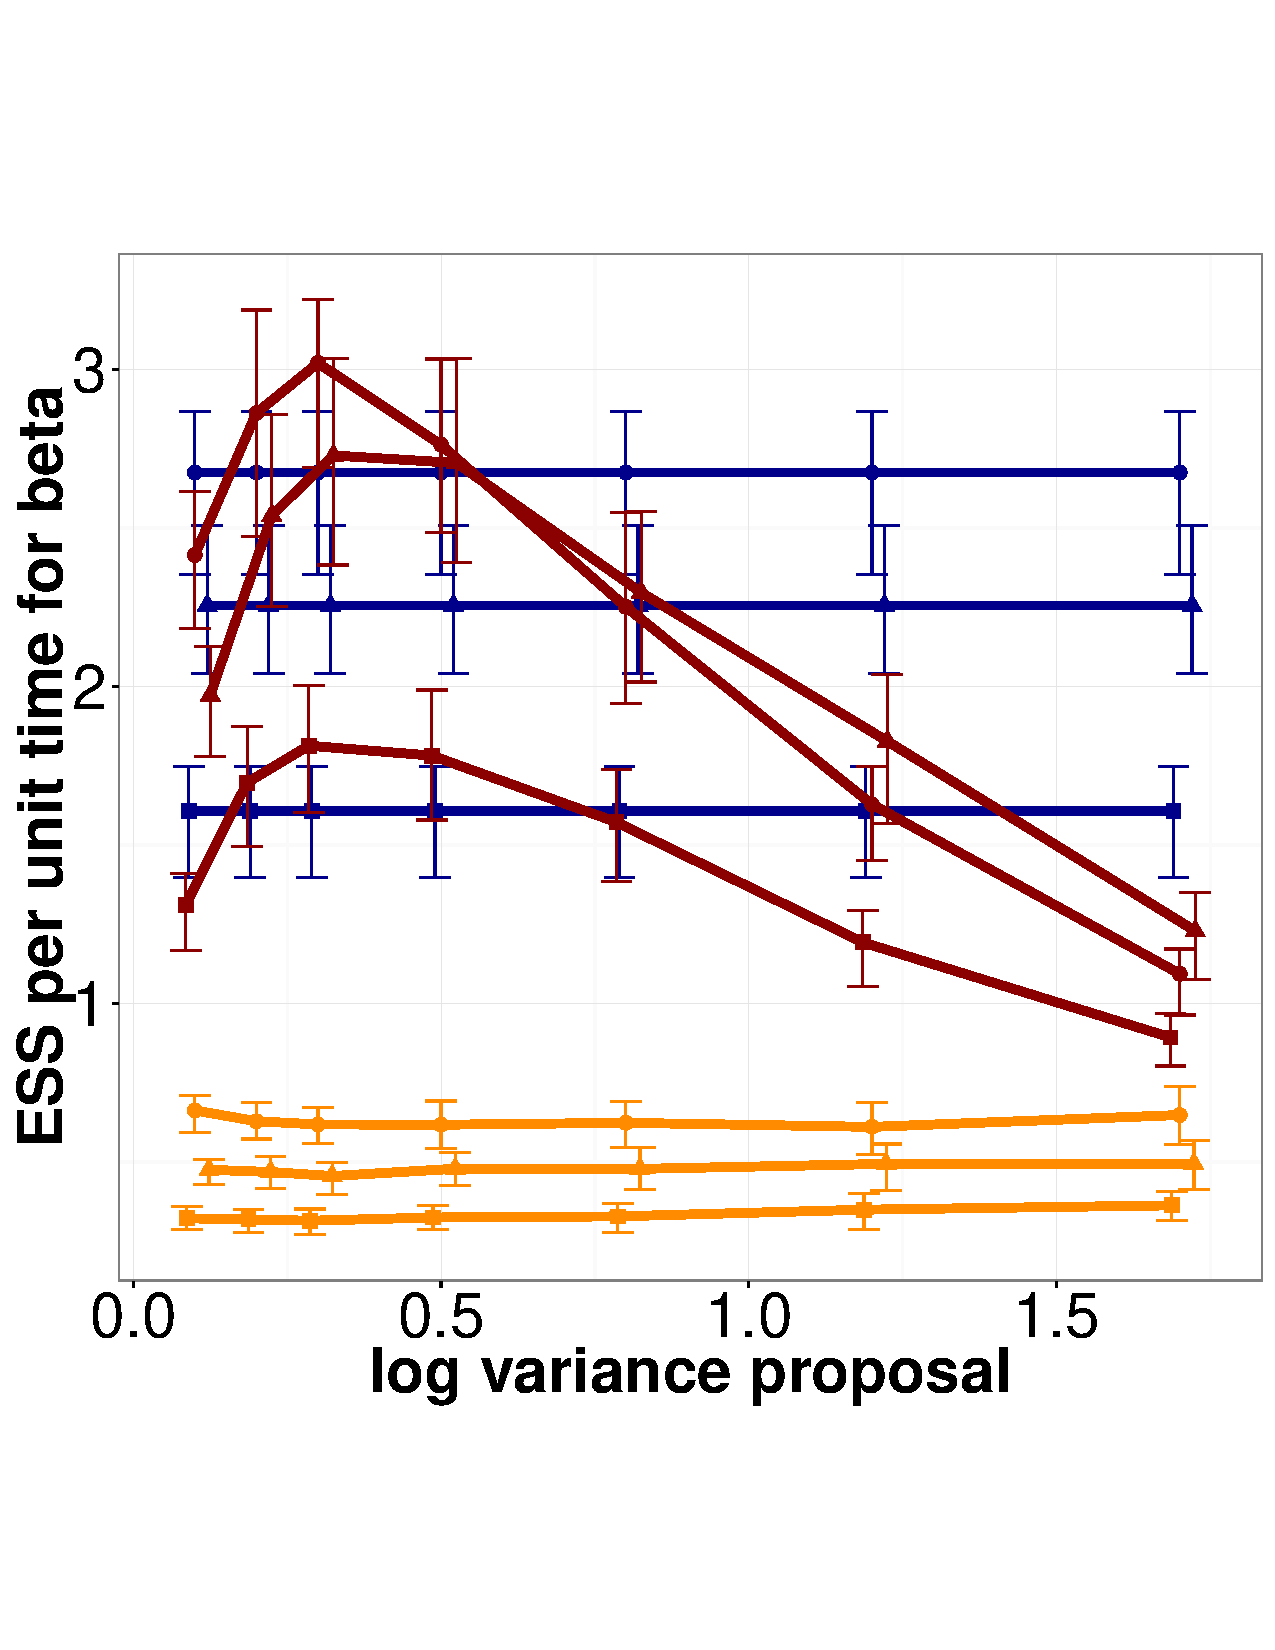
\includegraphics [width=0.70\textwidth, angle=0]{figs/q_5_beta.pdf}
    \vspace{-0 in}
     \label{fig:ESS_Q_5}
  \end{minipage}
    \caption{ESS/sec for Immigration model (dim 5)}
  \end{figure}

  \begin{figure}%[b]
  \centering
  \begin{minipage}[!hp]{0.45\linewidth}
  \centering
    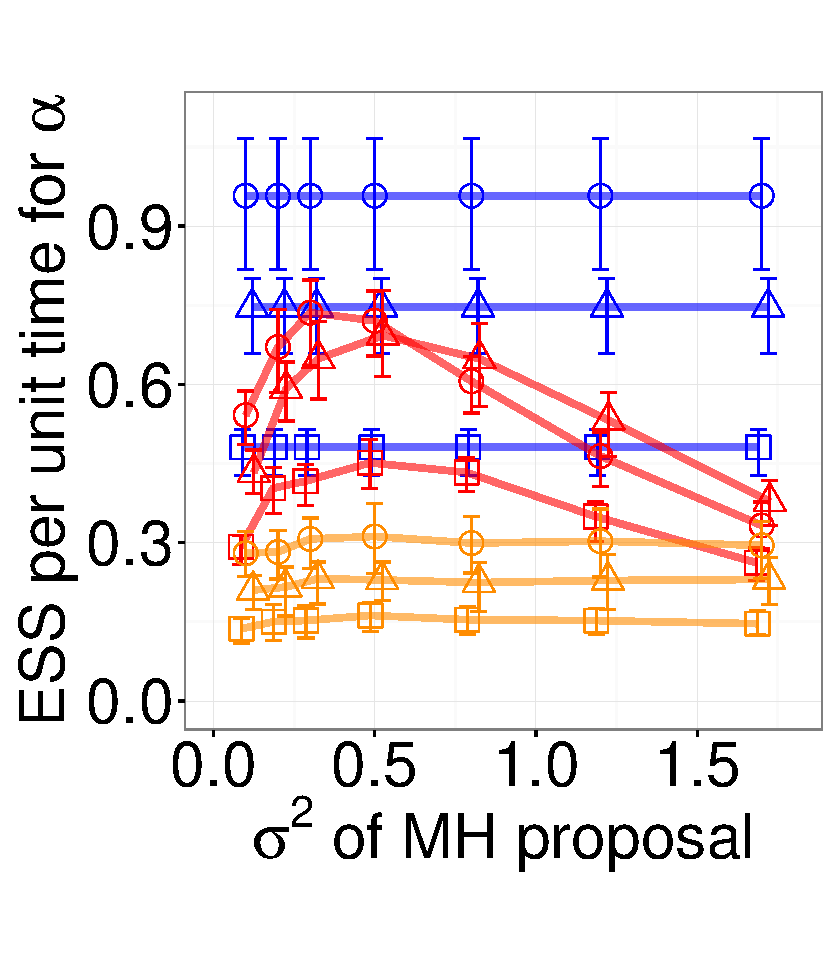
\includegraphics [width=0.70\textwidth, angle=0]{figs/q_10_alpha.pdf}
      \end{minipage}
  \begin{minipage}[!hp]{0.45\linewidth}
  \centering
    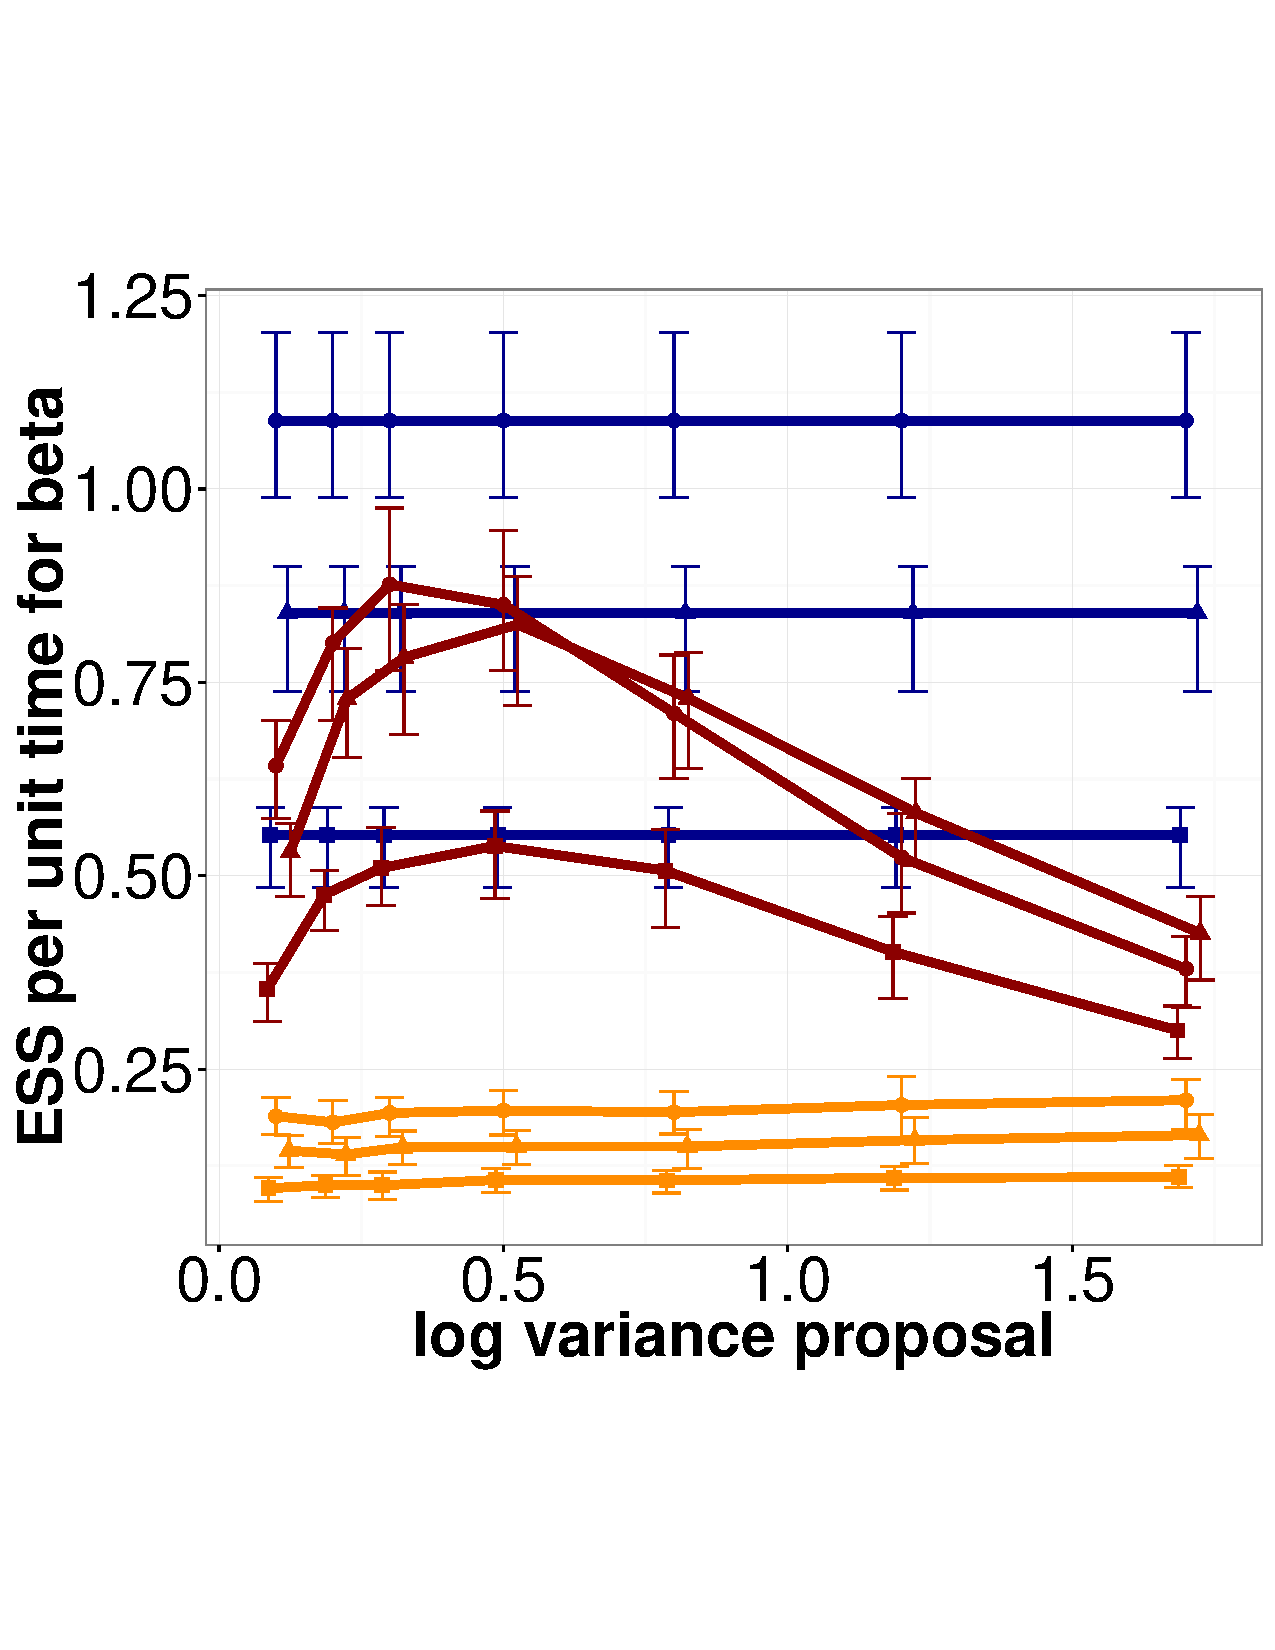
\includegraphics [width=0.70\textwidth, angle=0]{figs/q_10_beta.pdf}
    \vspace{-0 in}
     \label{fig:ESS_Q_10}
  \end{minipage}
    \caption{ESS/sec for Immigration model (dim 10)}
  \end{figure}

\begin{figure}
  \begin{minipage}[!hp]{0.45\linewidth}
  \centering
    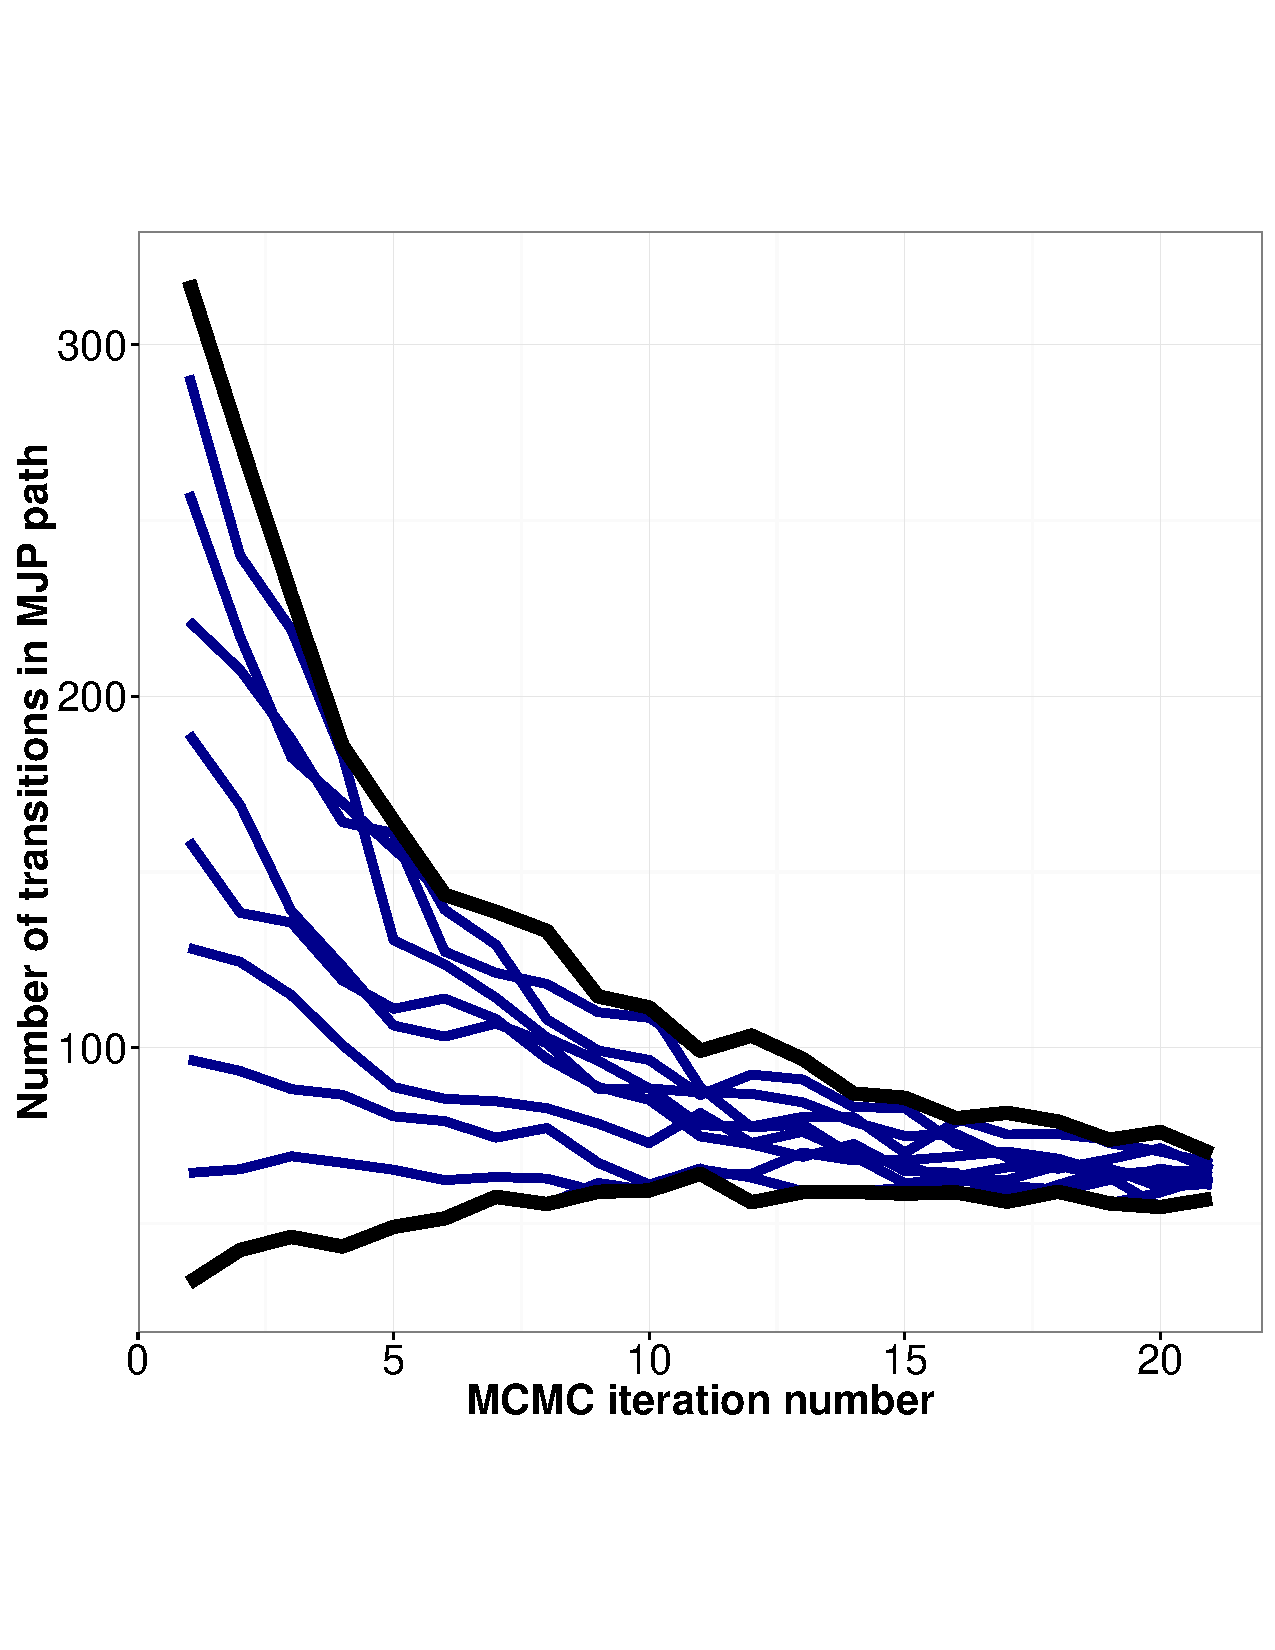
\includegraphics [width=0.70\textwidth, angle=0]{figs/q3_k2_path_transition.pdf}
    \vspace{-0 in}
    \caption{Trace plot of the number of MJP transitions for different initializatoins for immigration model.}
     \label{fig:ESS_EXP_TRANSITION}
  \end{minipage}
\end{figure}

  \begin{figure}%[b]
  \begin{minipage}[!hp]{0.45\linewidth}
  \centering
    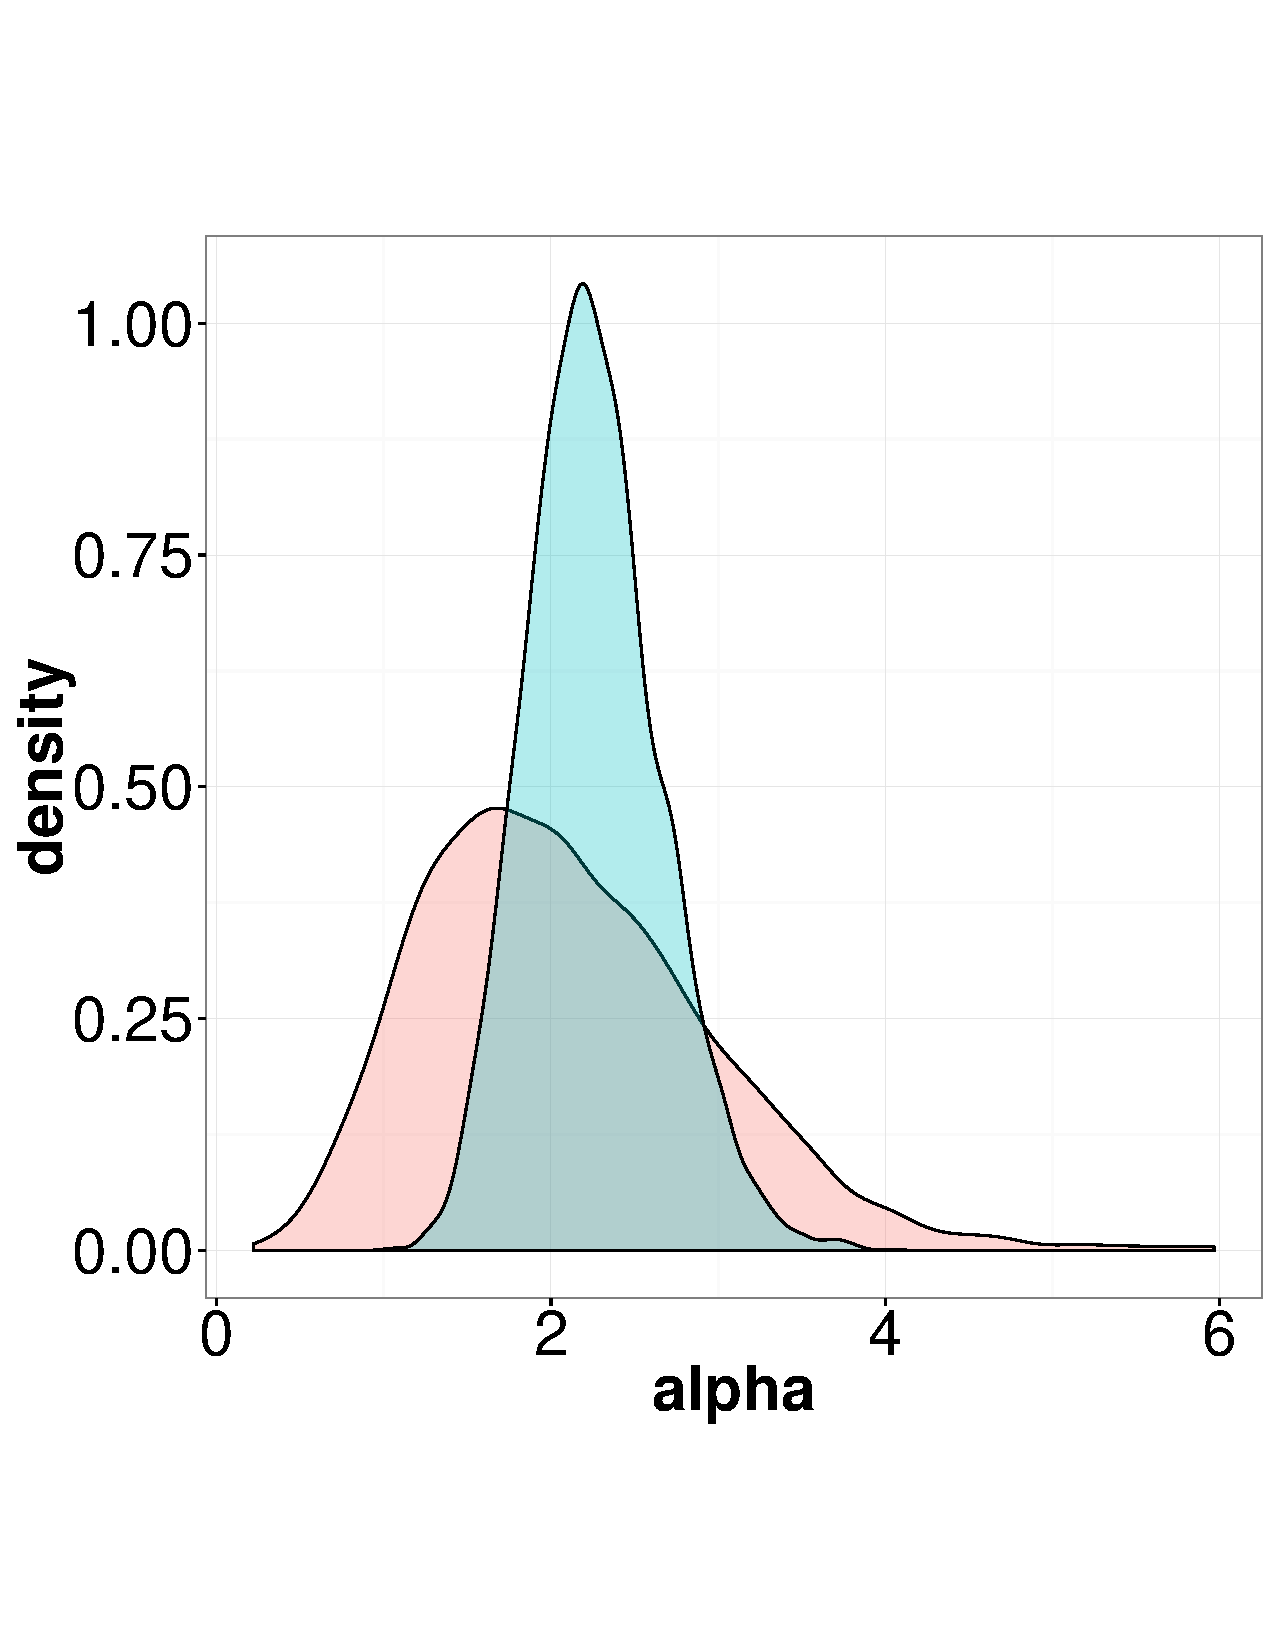
\includegraphics [width=0.70\textwidth, angle=0]{figs/dist_alpha.pdf}
    \vspace{-0 in}
     \label{fig:dist_alpha}
  \end{minipage}
  \begin{minipage}[!hp]{0.45\linewidth}
  \centering
    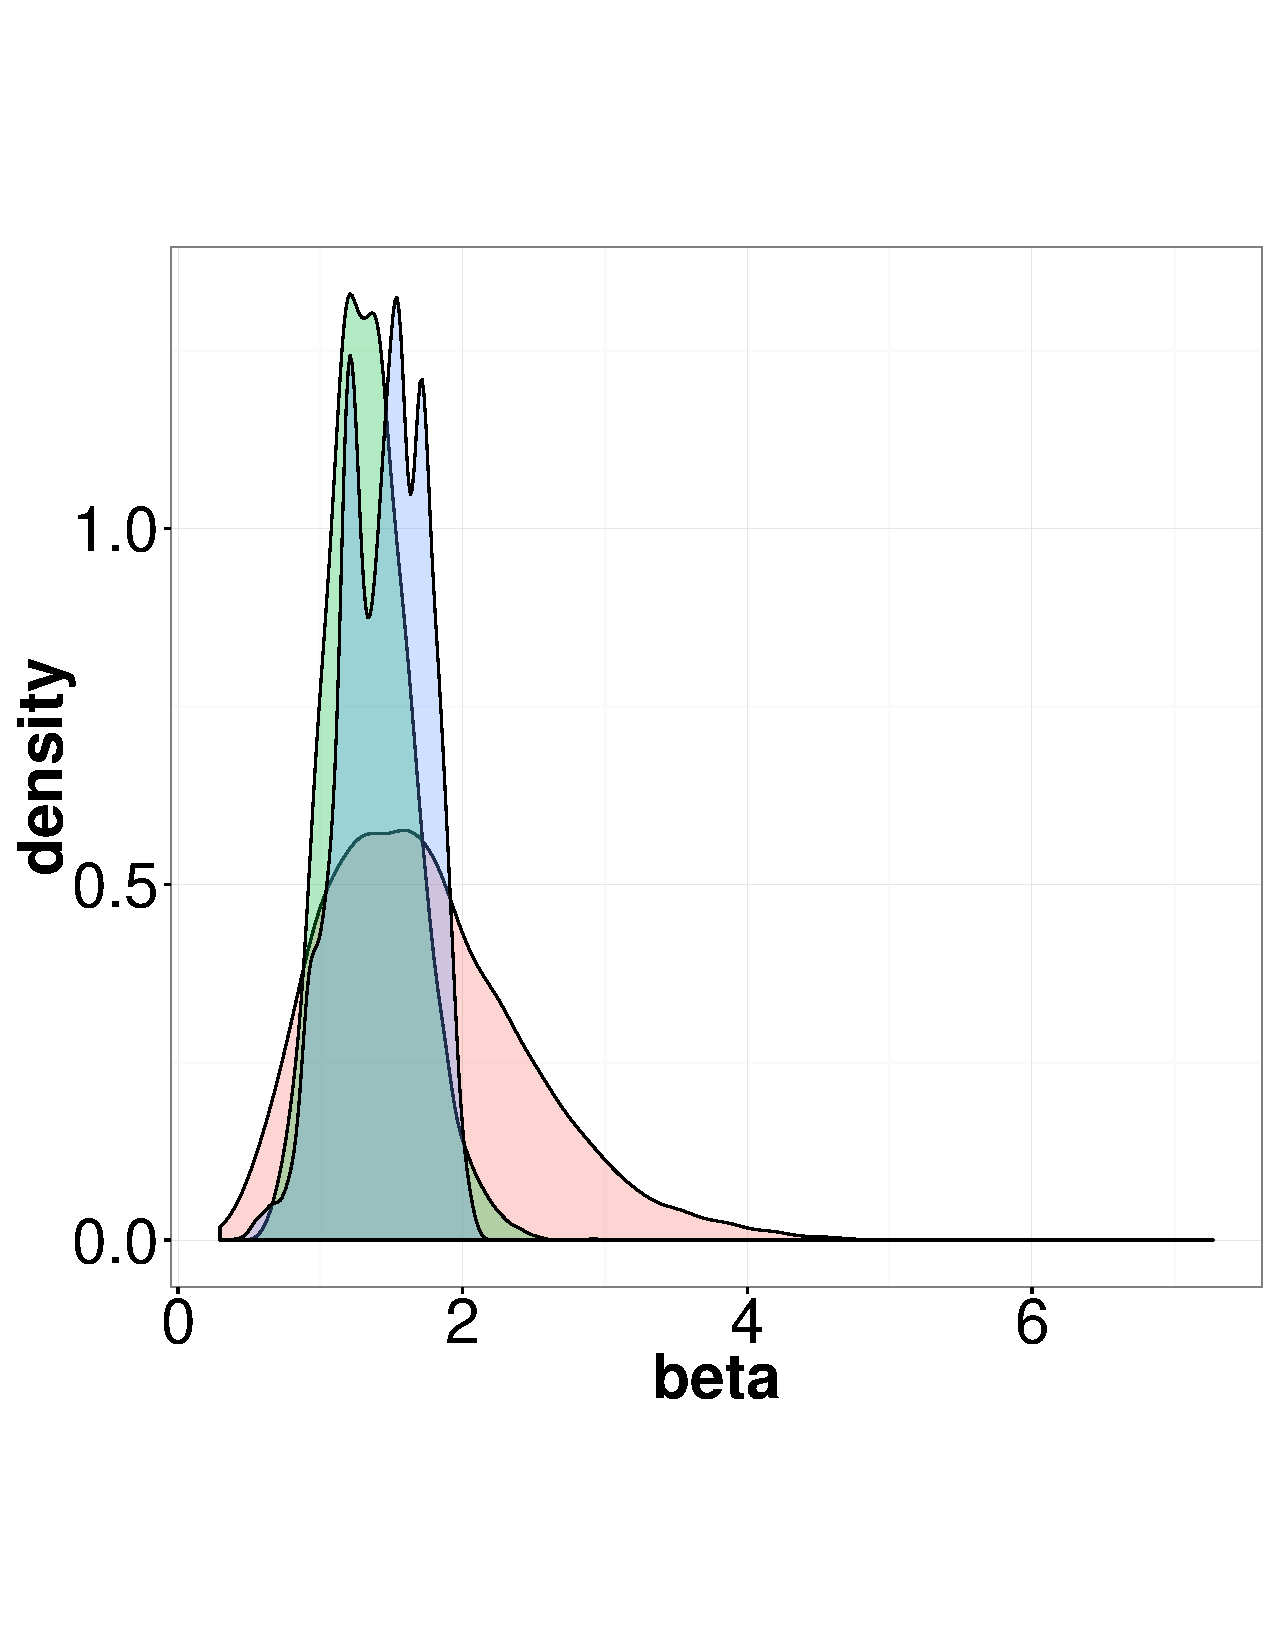
\includegraphics [width=0.70\textwidth, angle=0]{figs/dist_beta.pdf}
    \vspace{-0 in}
     \label{fig:dist_beta}
  \end{minipage}
    \caption{density}
  \end{figure}

  \begin{figure}%[b]
  \begin{minipage}[!hp]{0.45\linewidth}
  \centering
    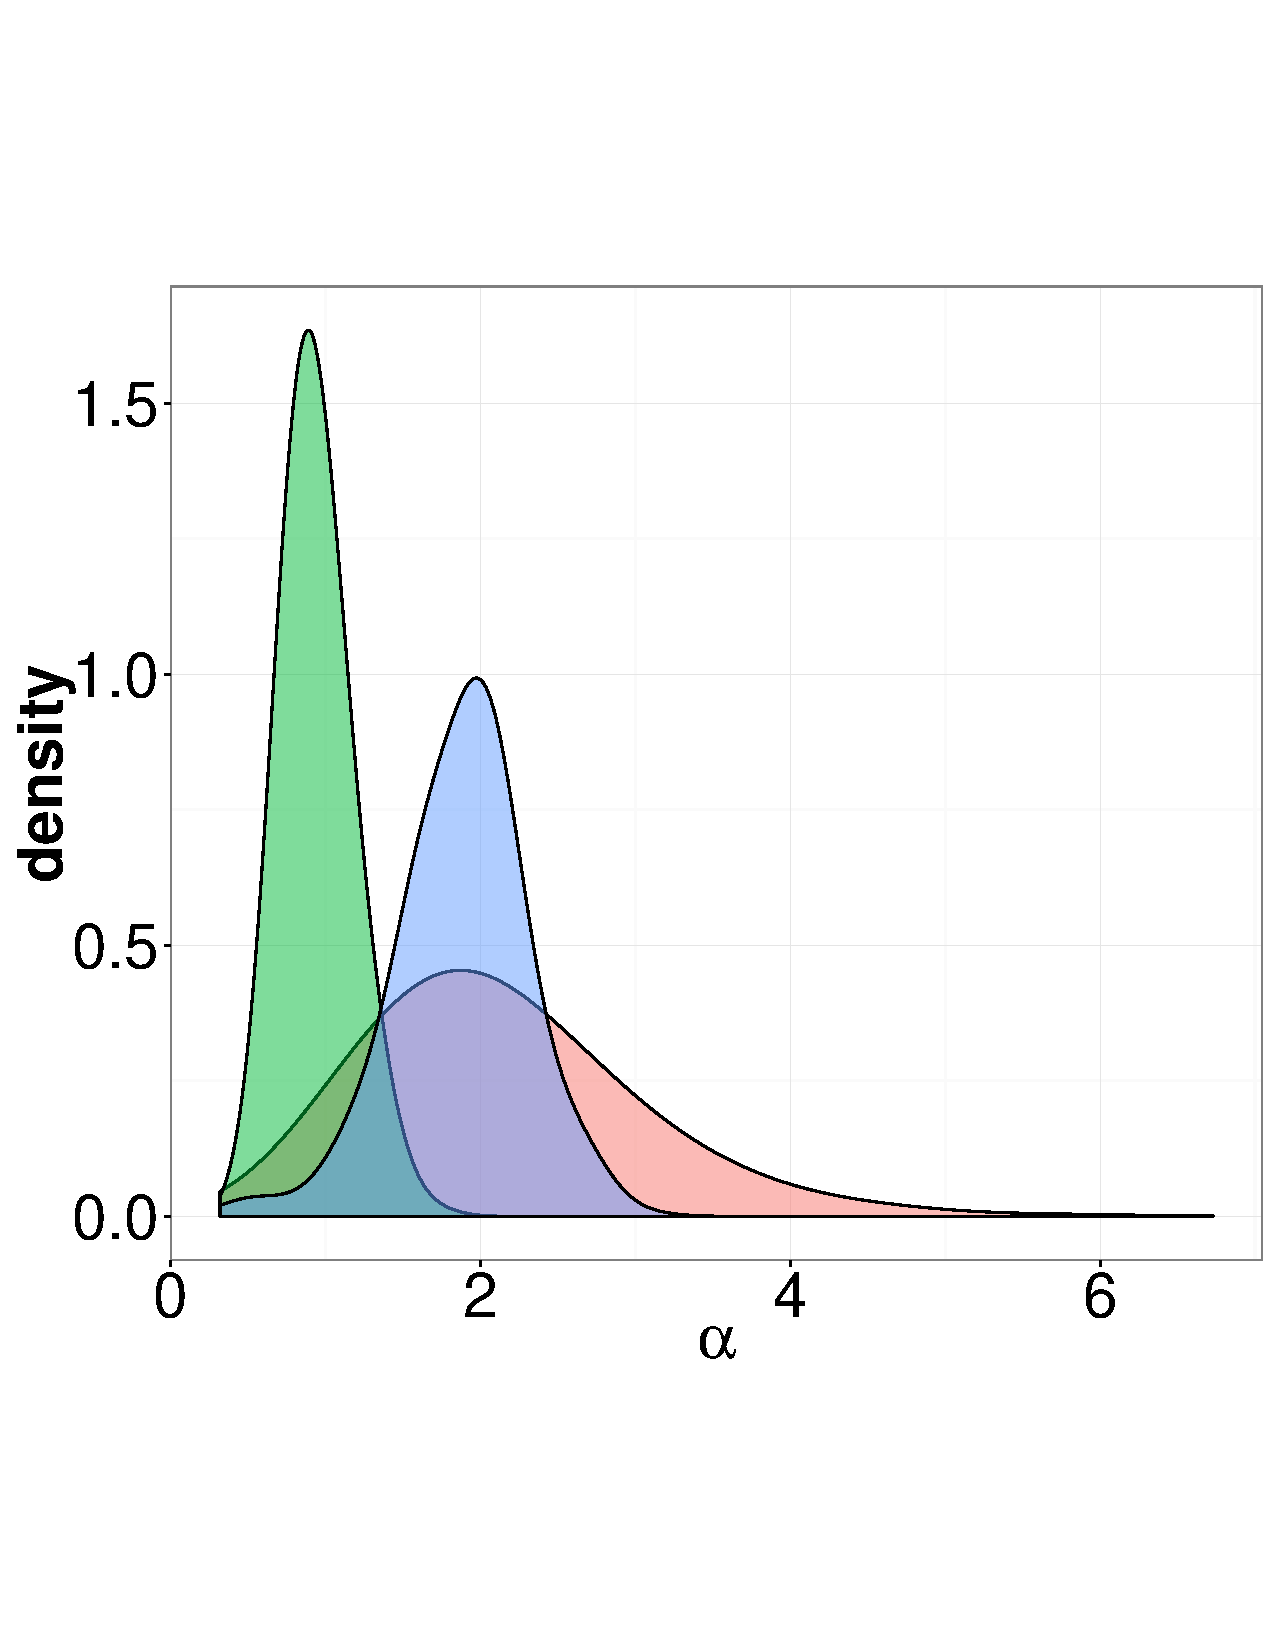
\includegraphics [width=0.70\textwidth, angle=0]{figs/hist_alpha.pdf}
    \vspace{-0 in}
     \label{fig:dist_alpha1}
  \end{minipage}
  \begin{minipage}[!hp]{0.45\linewidth}
  \centering
    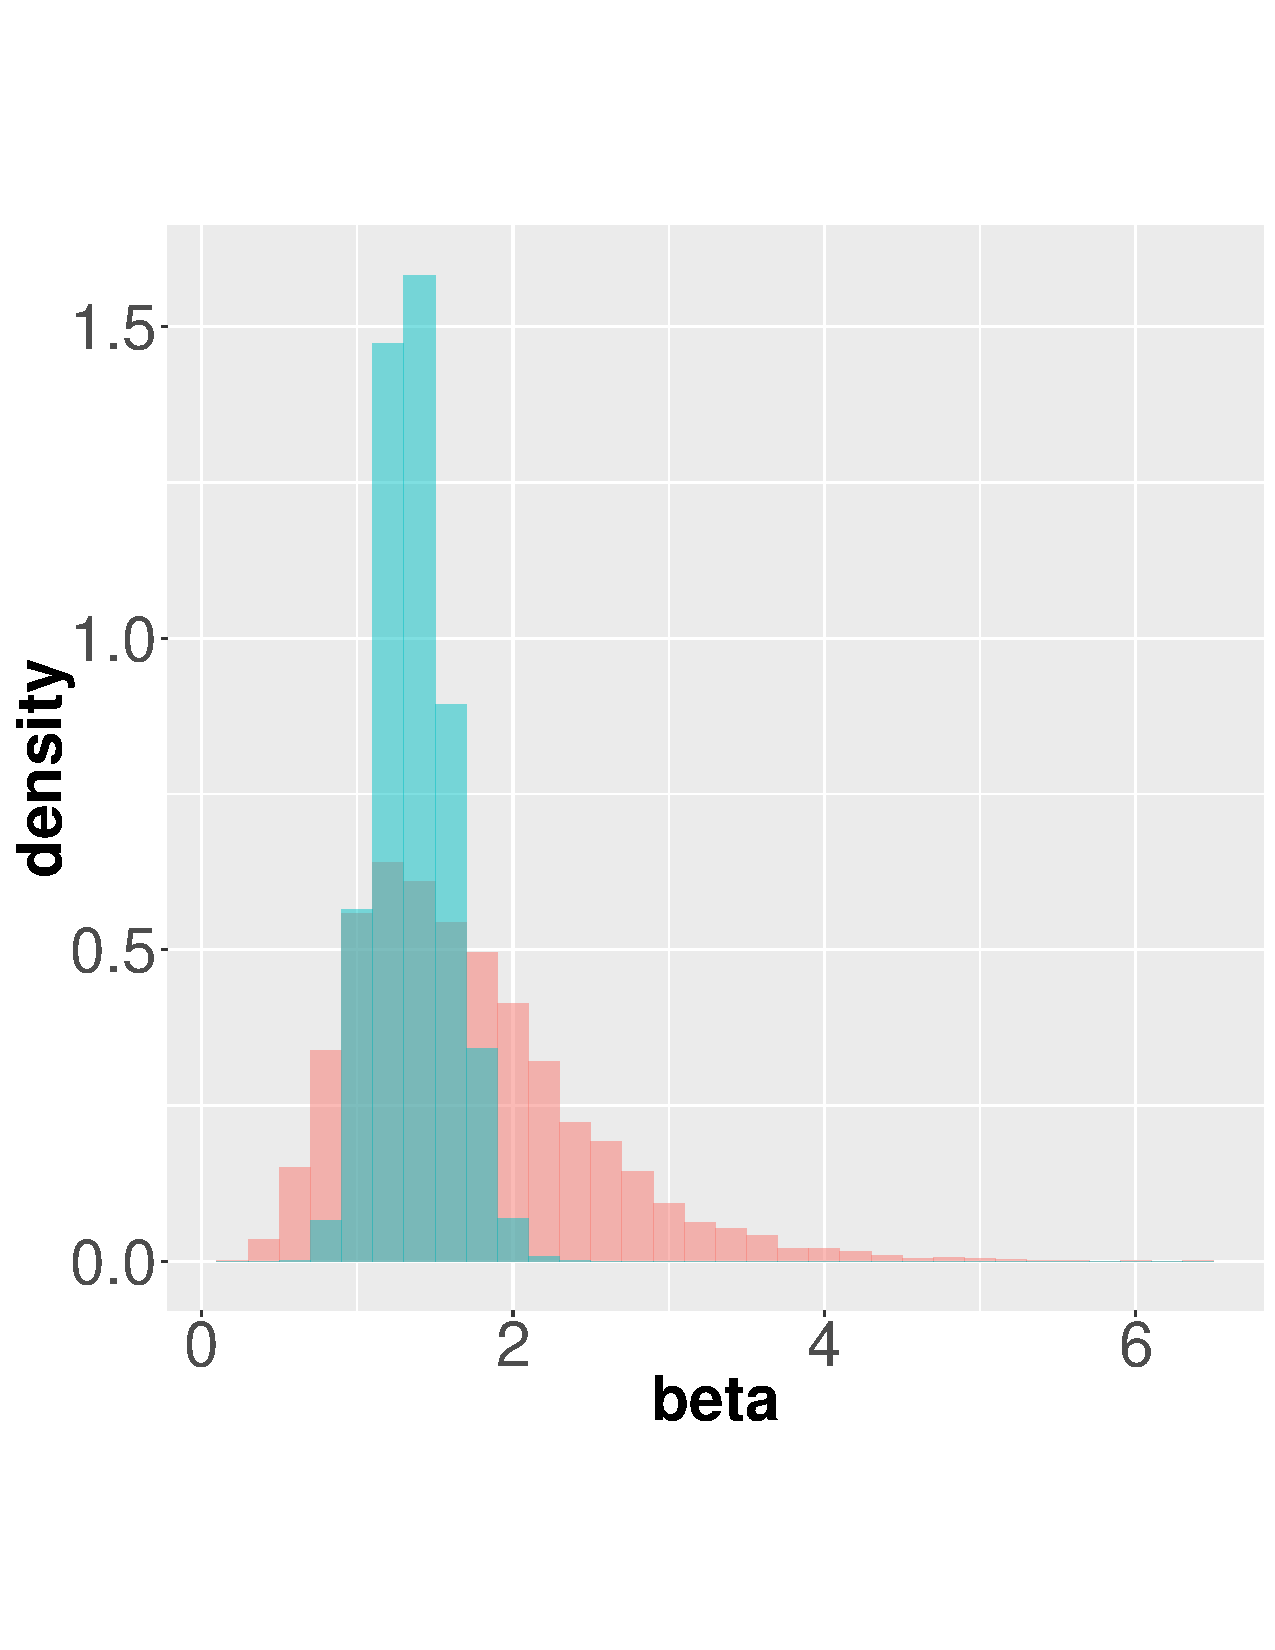
\includegraphics [width=0.70\textwidth, angle=0]{figs/hist_beta.pdf}
    \vspace{-0 in}
     \label{fig:hist_beta}
  \end{minipage}
    \caption{test}
  \end{figure}
  

\section{DNA evolution JC69 model }~
  \begin{figure}[H]
  \centering
  \begin{minipage}[!hp]{0.45\linewidth}
  \centering
    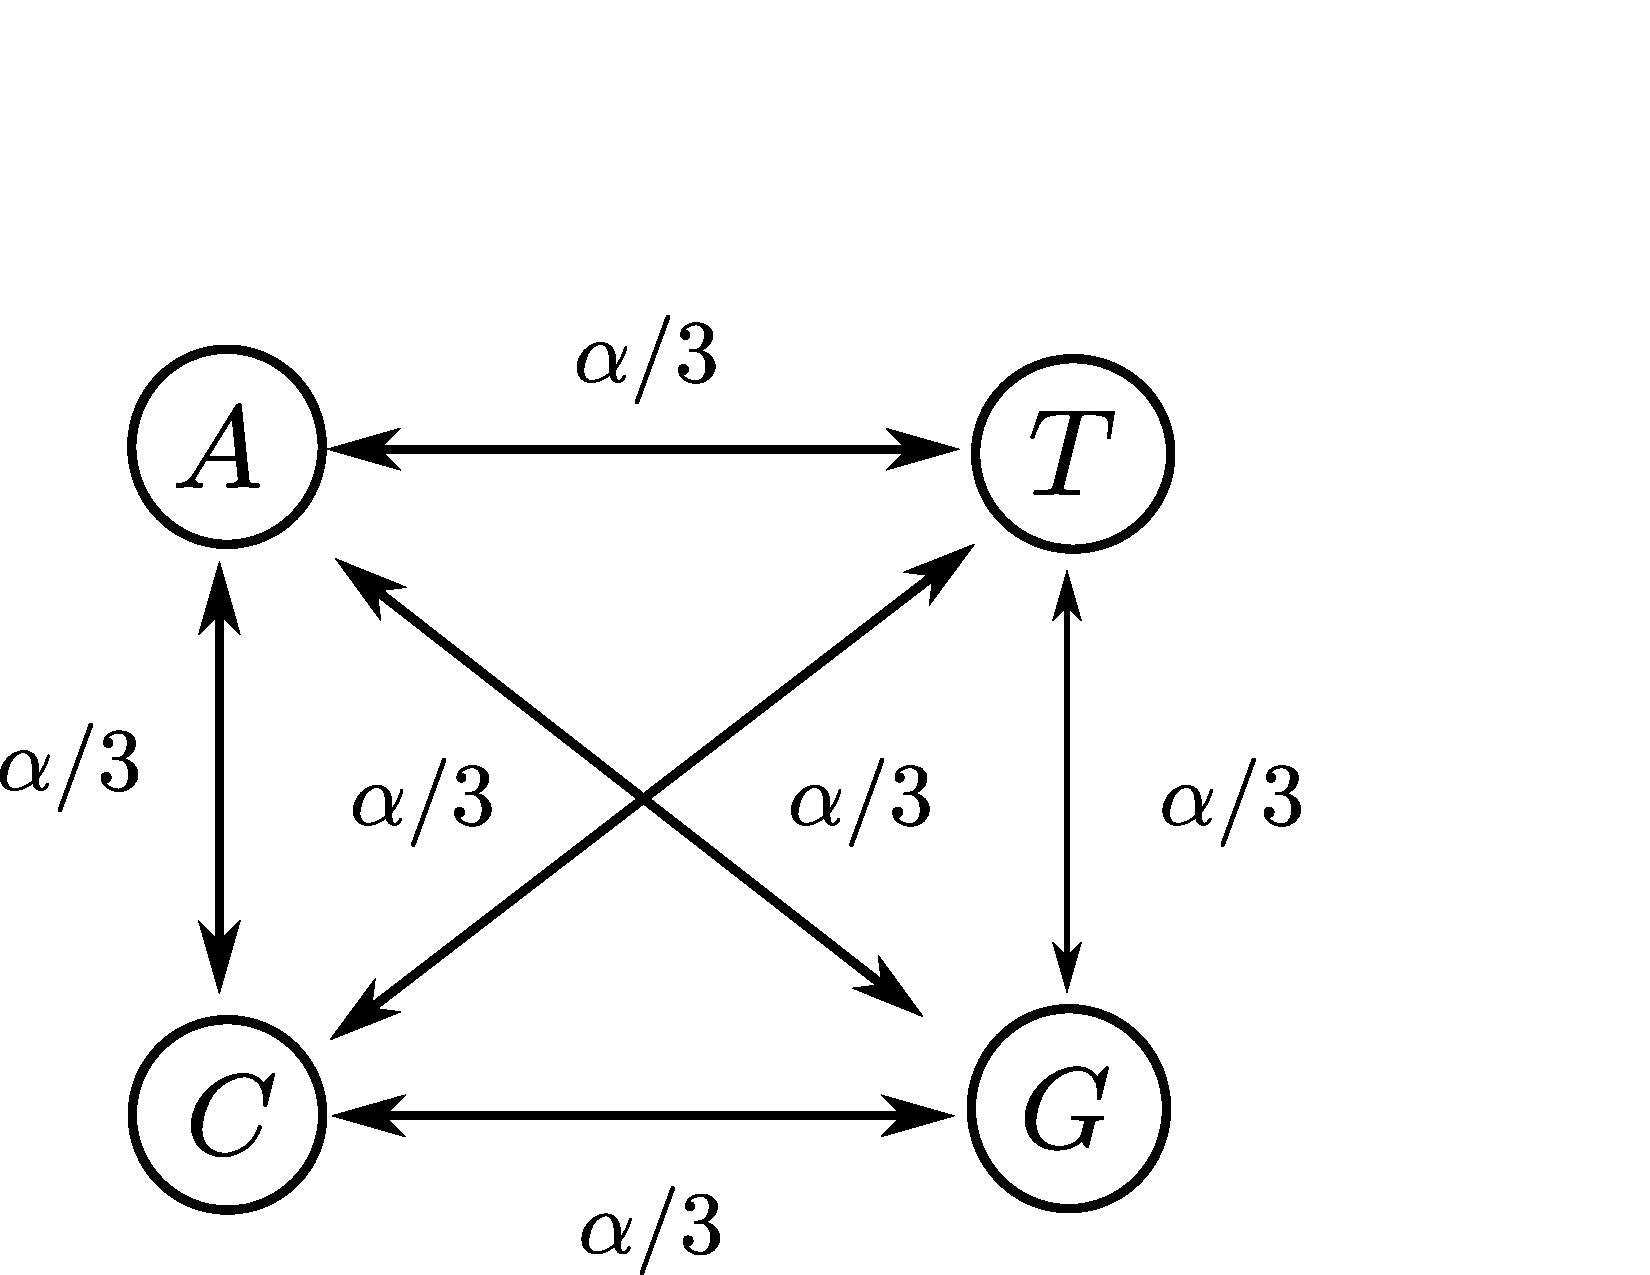
\includegraphics [width=0.70\textwidth, angle=0]{figs/jc_model.pdf}
      \end{minipage}
    \caption{exp model}
  \end{figure}

JC69 is the simplest substitution model. There are several assumptions. It assumes equal base frequencies and equal mutation rates. The only parameter of this model is $\alpha$. The overall substitution rate is therefore $3\alpha$. The state space is $\{1, 2, 3, 4\}$, representing $\{A, T, C, G\}$.\noindent Assume: $S = [S_0,S_1, ...,S_N] \;, T = [t_0(t_{start}), t_1,...,t_N, t_{N+1}(t_{end})]$, and y as observations.\\
$$A_i =: A_{i,i} = -3\alpha, \; \; i =0,1,...,N$$ $$A_{i, j} = \alpha, \; \; i \neq j.$$
If we assume the prior of $\alpha$ is $Gamma(\mu,\lambda)$\\
$$p(\alpha) = \frac{\lambda^\mu}{\Gamma(\mu)}\alpha^{\mu -1}e^{-\lambda \alpha} $$.
Then we can get the posterior distribution $$f(\alpha | s_0,S,T)$$ as follows.
$$ f(\alpha| s_0,S,T) \propto \exp(-(\lambda + 3(t_{end} - t_{start}))\alpha) \alpha^{\mu + N -1} .$$
$\alpha | s_0,S,T$ is following $Gamma(\mu+ N,\lambda + 3(t_{end} - t_{start}))$\\
\section{Experiments}
In the following, we evaluate a Python implementation of our algorithms compared to other exact samplers which include Gibbs sampler and Particle MCMC sampler. We consider three different dimensions which are 3, 5, and 10 and three different k which are 1.5, 2, and 3. We generated random parameters $\alpha$, $\beta$ from prior distributions ($Gamma(3,2), Gamma(5, 2)$), and used this to construct the transition matrix A. Then we generate an MJP trajectory with a uniform initial distribution over states. The state of this MJP trajectory was observed via a Normal distribution with mean equal to the value of state and variance 1, and posterior samples given the observations were produced by a Python implementation of our algorithm. 100 MCMC runs were performed, each run consisting of 10000(Varies among different dimensions) iterations. For each run, the number of transitions as well as the time spent was calculated, and effective sample sizes (ESSs) of these statistics (the number of independent samples with the same `information' as the correlated MCMC samples) were calculated using R-CODA (Plummer et al., 2006). The overall ESS of a run is defined to be the mean ESS across all these ESSs.

  \begin{figure}%[b]
  \begin{minipage}[!hp]{0.45\linewidth}
  \centering
    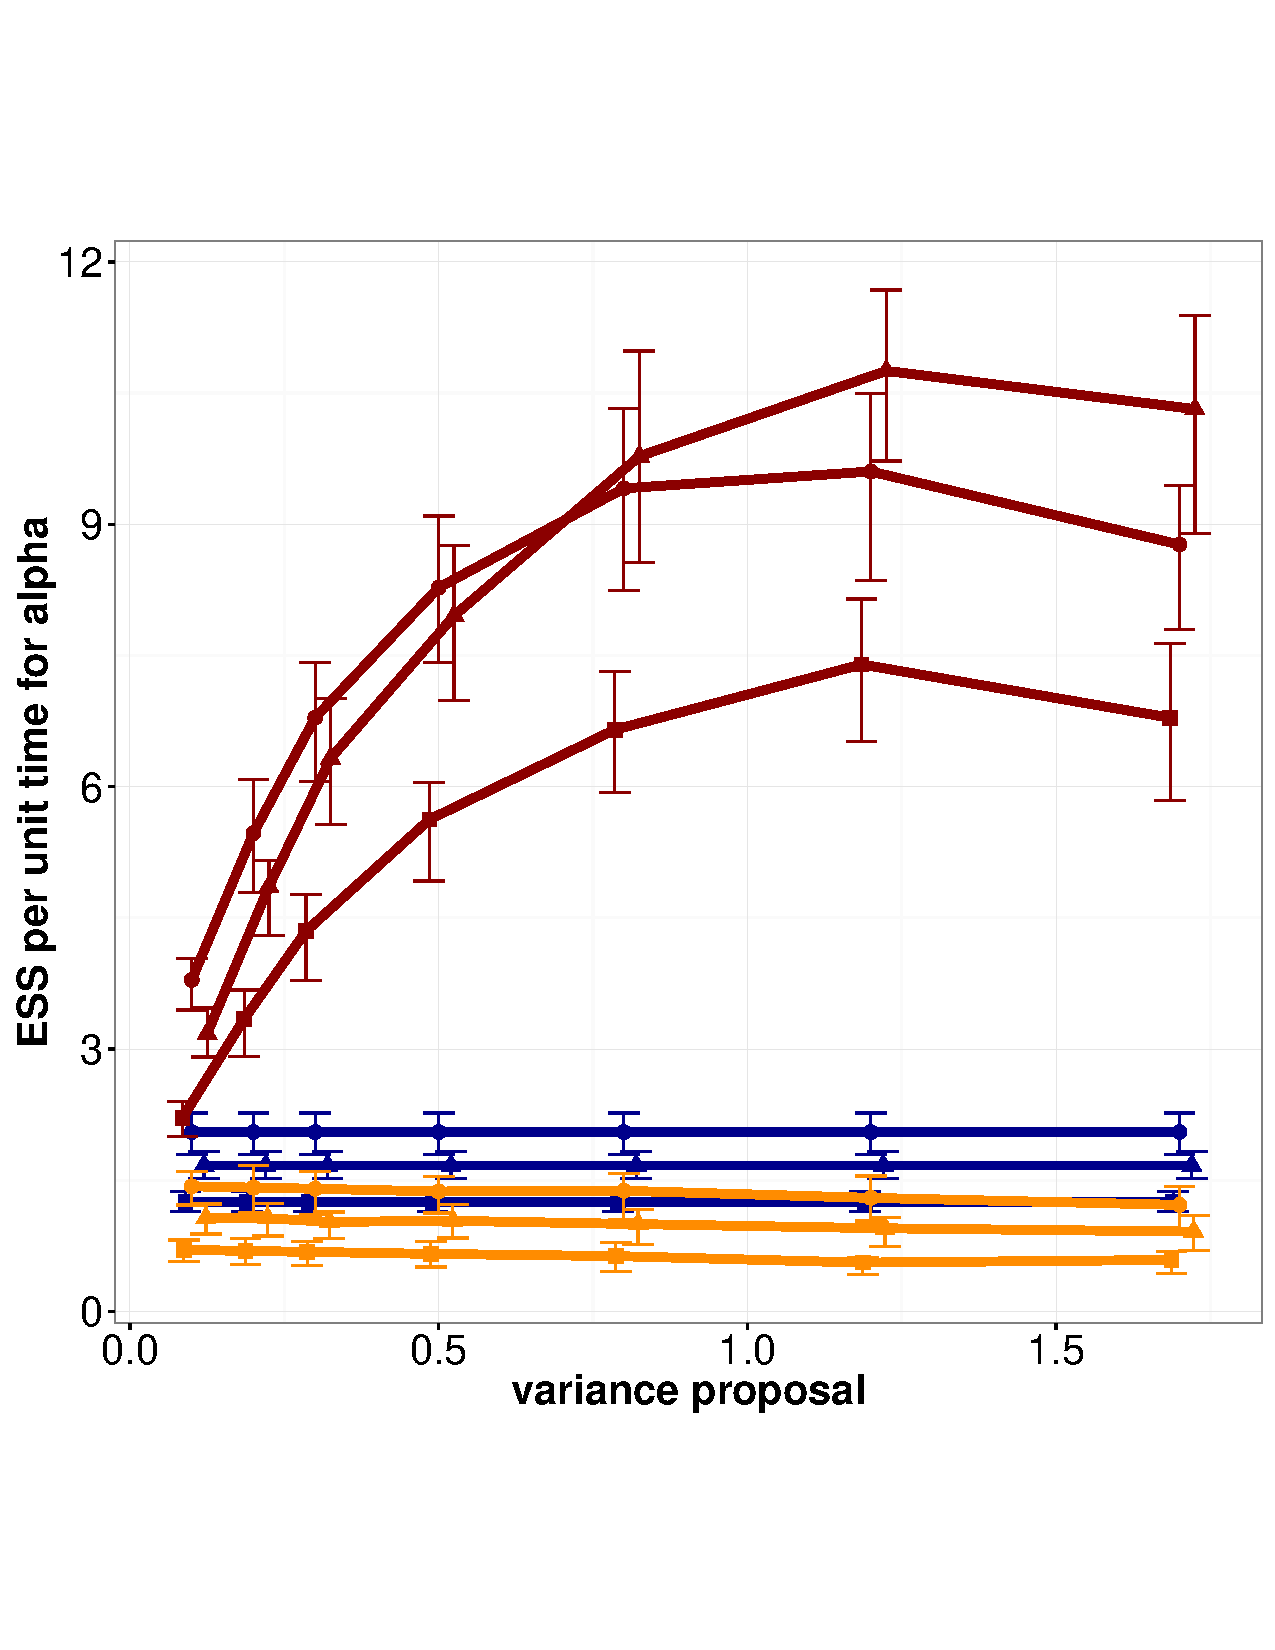
\includegraphics [width=0.70\textwidth, angle=0]{figs/jc.pdf}
    \vspace{-0 in}
    \caption{ESS/sec for JC69 Model }
     \label{fig:ESS_JC}
  \end{minipage}
  \end{figure}



\section{Immigration models with capacity with piece wise constant rate}~
We consider the Queuing model, with piece wise constant transition rate. 
\noindent Assume: $S = [S_0,S_1, ...,S_N] \;, T = [t_0(t_{start}), t_1,...,t_N, t_{N+1}(t_{end})]$, and y as observations.\\
Now, let's consider a immigration model as follows. State space is $\{0, 1, 2, ..., N - 1\}$, representing the total population. The transition matrix is defined as follows. 
$$A_i(t) =: A_{i,i}(t) = -(\alpha + i\beta)w(t), \; \; i =0,1,...,N$$ $$A_{i, i+1}(t) = \alpha w(t), \; \; i =0,1,...,N-1,$$ $$A_{i, i-1}(t)  = \beta w(t), \; \;  i =1,...,N.$$
$w(t)$ is a piece wise constant function. $w(t) = w_i, \; t \in [\l_i, l_{i + 1}), i = 1,2,3,..., K.$\\
We already know the conditional density(given $\alpha,\; \beta$) of a MJP trajectory $(s_0, S, T)$ in time interval $[t_{start}, t_{end}]$, with $S=(s_1, s_2,..., s_k)$, $T=(t_1, t_2,..., t_k)$. 
$$f(s_0,S,T| \alpha, \beta) = \prod_{i=0}^{k-1} A_{s_i, s_{i+1}}(t_i) \exp(\sum_{i=0}^{k} A_{s_i}(t_i)(t_{i+1} - t_{i})), $$
where $t_0 = t_{start}$, $t_{k+1} = t_{end}.$\\
Let's denote some notations here.\\
$$U(s_0, S, T):= \sum_{i=0}^{k-1} \mathbb{I}_{\{s_{i+1} - s_i = 1\}}.$$
$$D(s_0, S, T):= \sum_{i=0}^{k-1} \mathbb{I}_{\{s_{i+1} - s_i = -1\}}.$$
Call them U and D for short.
Let's denote the total time when the trajectory state stays at state i as $\tau_i$, i.e. $\tau_i = \sum_{j=0}^{k} (t_{j+1} -t_j)\mathbb{I}_{\{s_j = i\}}$, then $\sum_{i=0}^k (t_{i+1} - t_i)s_i = \sum_{i=0}^N \tau_ii.$\\

$$f(s_0,S,T| \alpha, \beta) \propto \exp(\sum_{r = 0}^{K}-w_r\alpha(l_{r + 1} - l_{r}- \tau_N^r) )\alpha^U \cdot  \exp(-\int_{t_s}^{t_{e}}(S(t)w(t)\beta)  \beta^D$$\\
If we assume the prior of $\alpha$, and $\beta$ are $Gamma(\mu,\lambda)$, $Gamma(\omega, \theta)$, which are independent with each other. \\
$$p(\alpha) = \frac{\lambda^\mu}{\Gamma(\mu)}\alpha^{\mu -1}e^{-\lambda \alpha}. $$
$$p(\beta) = \frac{\theta^\omega}{\Gamma(\omega)}\beta^{\omega -1}e^{-\theta \beta}. $$
Then we can get the posterior distribution $$f(\alpha, \beta | s_0,S,T)$$ as follows.
$$ f(\alpha, \beta | s_0,S,T) \propto \exp(-(\lambda +\sum_{r = 0}^{K}w_r\alpha(l_{r + 1} - l_{r}- \tau_N^r))\alpha) \alpha^{\mu + U -1} \cdot \exp(-(\int_{t_{s}}^{t_{e}}(S(t)w(t) + \theta)\beta) \beta^{\omega+ D -1}.$$
It means that the posterior distributions of $\alpha$, $\beta$ are still independent. \\
$\alpha | s_0,S,T$ is following $Gamma(\mu+ U,\lambda +\sum_{r = 0}^{K}w_r\alpha(l_{r + 1} - l_{r}- \tau_N^r)  )$\\
$\beta | s_0,S,T$ is following $Gamma(\omega+ D,\int_{t_s}^{t_{e}}(S(t)w(t) + \theta)$.\\
Such immigration models have perfectly conjugate posterior distributions when we assign $\gamma$ priors to $\alpha$ and $\beta$. We apply our Metropolis Hasting algorithms on such models to compare the performance with the performance of Gibbs Sampling algorithm.

\subsection{Experiments}
In the following, we evaluate a Python implementation of our algorithms compared to the Gibbs sampler. We consider three different dimensions which are 3, 5, and 10 and three different k which are 1.5, 2, and 3. We generated random parameters $\alpha$, $\beta$ from prior distributions ($Gamma(3,2), Gamma(5, 2)$). We set $w$ as $(1, 2, 3, 4)$ and $l$ as $(0, 5, 10, 15, 20)$   We used this to construct the transition matrix A. Then we generate an MJP trajectory with a uniform initial distribution over states. The state of this MJP trajectory was observed via a Normal distribution with mean equal to the value of state and variance 1, and posterior samples given the observations were produced by a Python implementation of our algorithm. 100 MCMC runs were performed, each run consisting of 5000(Varies among different dimensions) iterations. For each run, the number of transitions as well as the time spent was calculated, and effective sample sizes (ESSs) of these statistics (the number of independent samples with the same `information' as the correlated MCMC samples) were calculated using R-CODA (Plummer et al., 2006). The overall ESS of a run is defined to be the mean ESS across all these ESSs.

  \begin{figure}%[b]
  \centering
  \begin{minipage}[!hp]{0.45\linewidth}
  \centering
    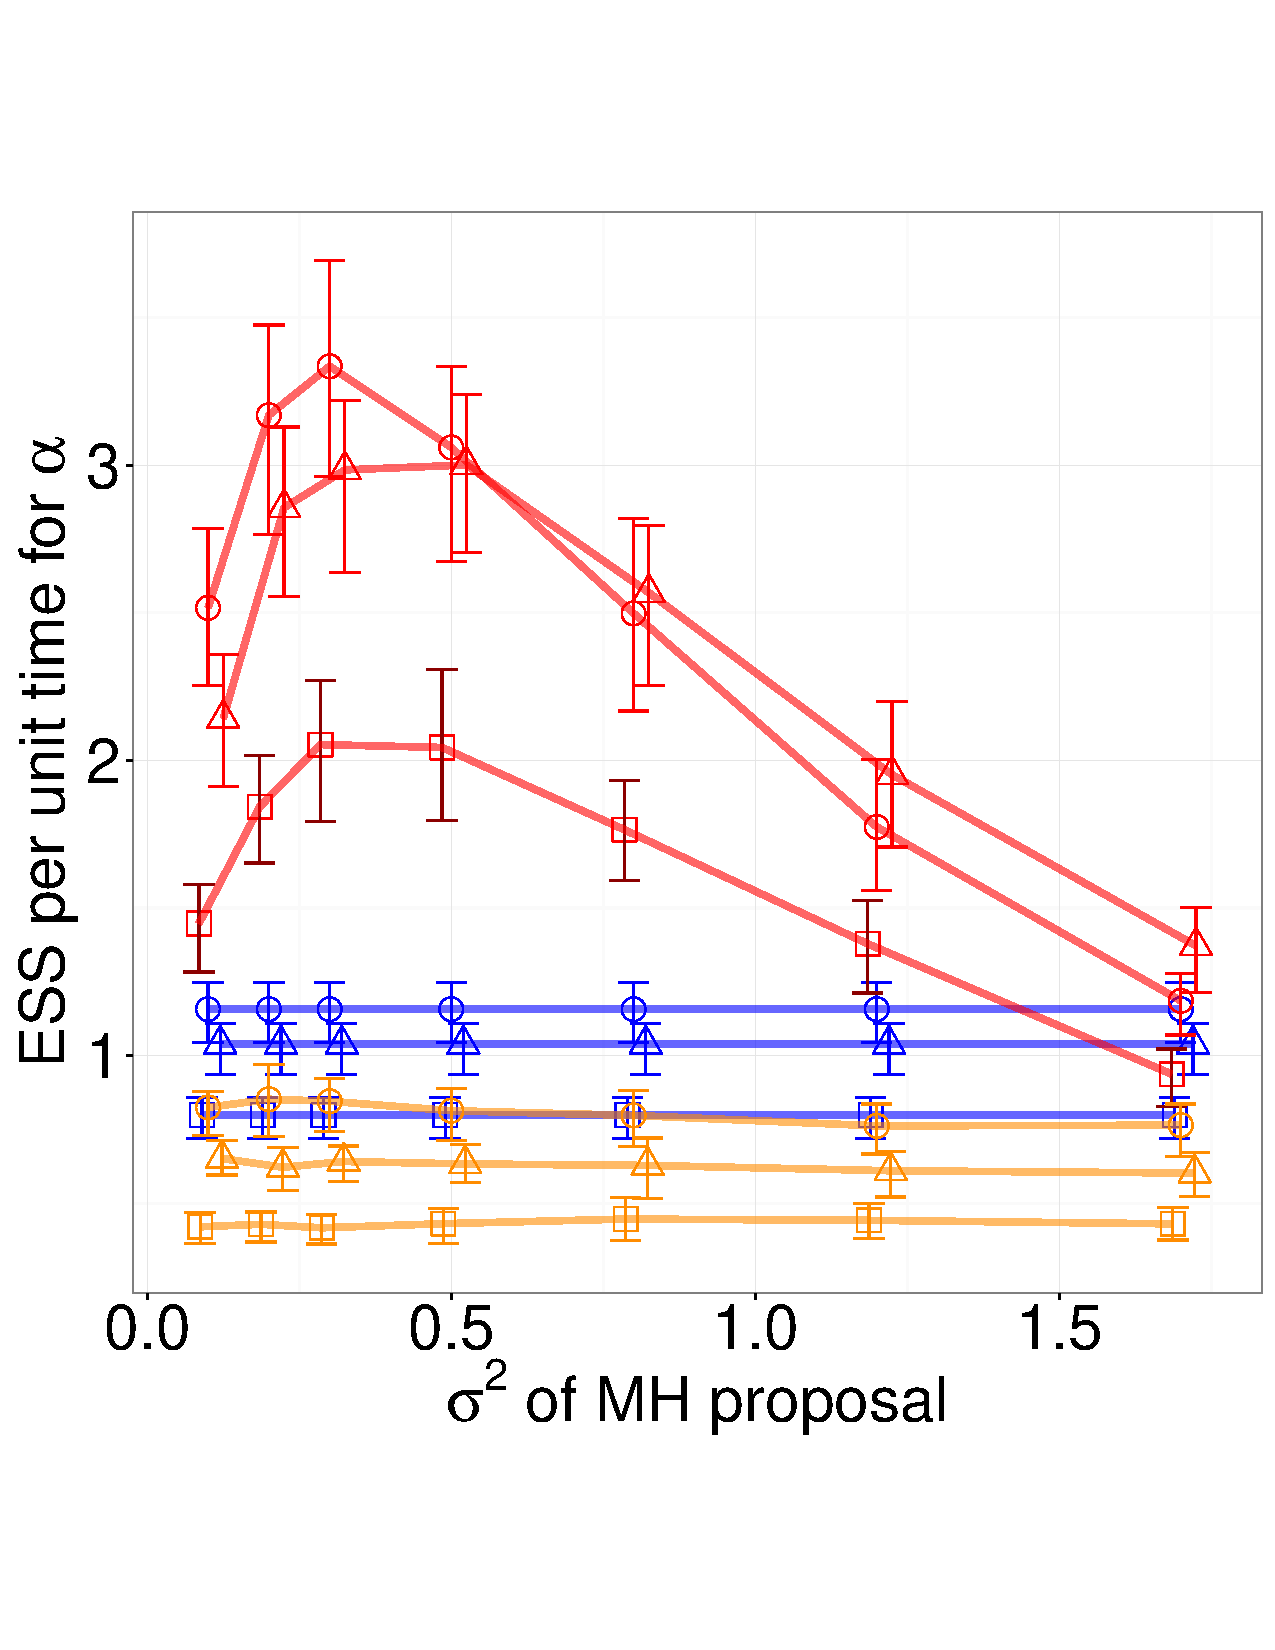
\includegraphics [width=0.70\textwidth, angle=0]{figs/pc_3_alpha.pdf}
      \end{minipage}
  \begin{minipage}[!hp]{0.45\linewidth}
  \centering
    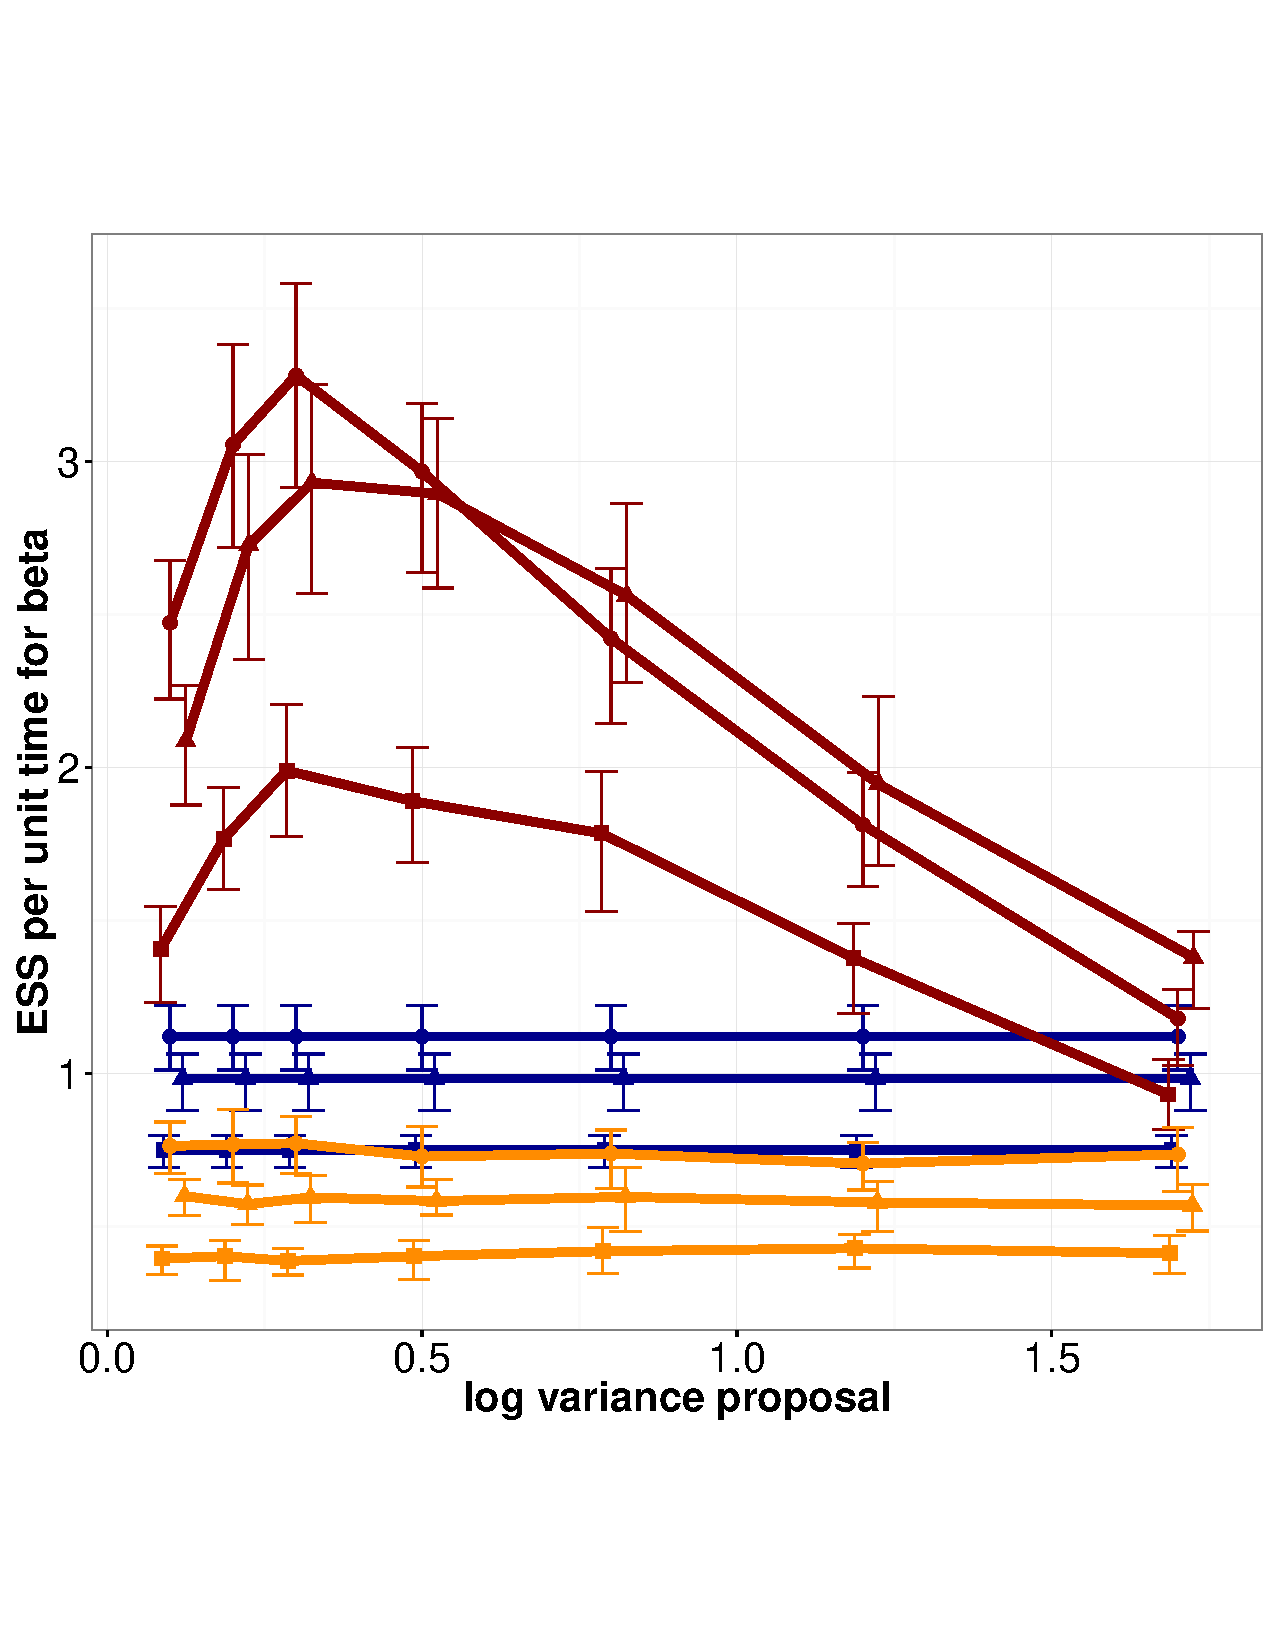
\includegraphics [width=0.70\textwidth, angle=0]{figs/pc_3_beta.pdf}
    \vspace{-0 in}
     \label{fig:ESS_Q_3}
  \end{minipage}
    \caption{ESS/sec for NH Immigration model (dim 3)}
  \end{figure}
  \begin{figure}%[b]
  \centering
  \begin{minipage}[!hp]{0.45\linewidth}
  \centering
    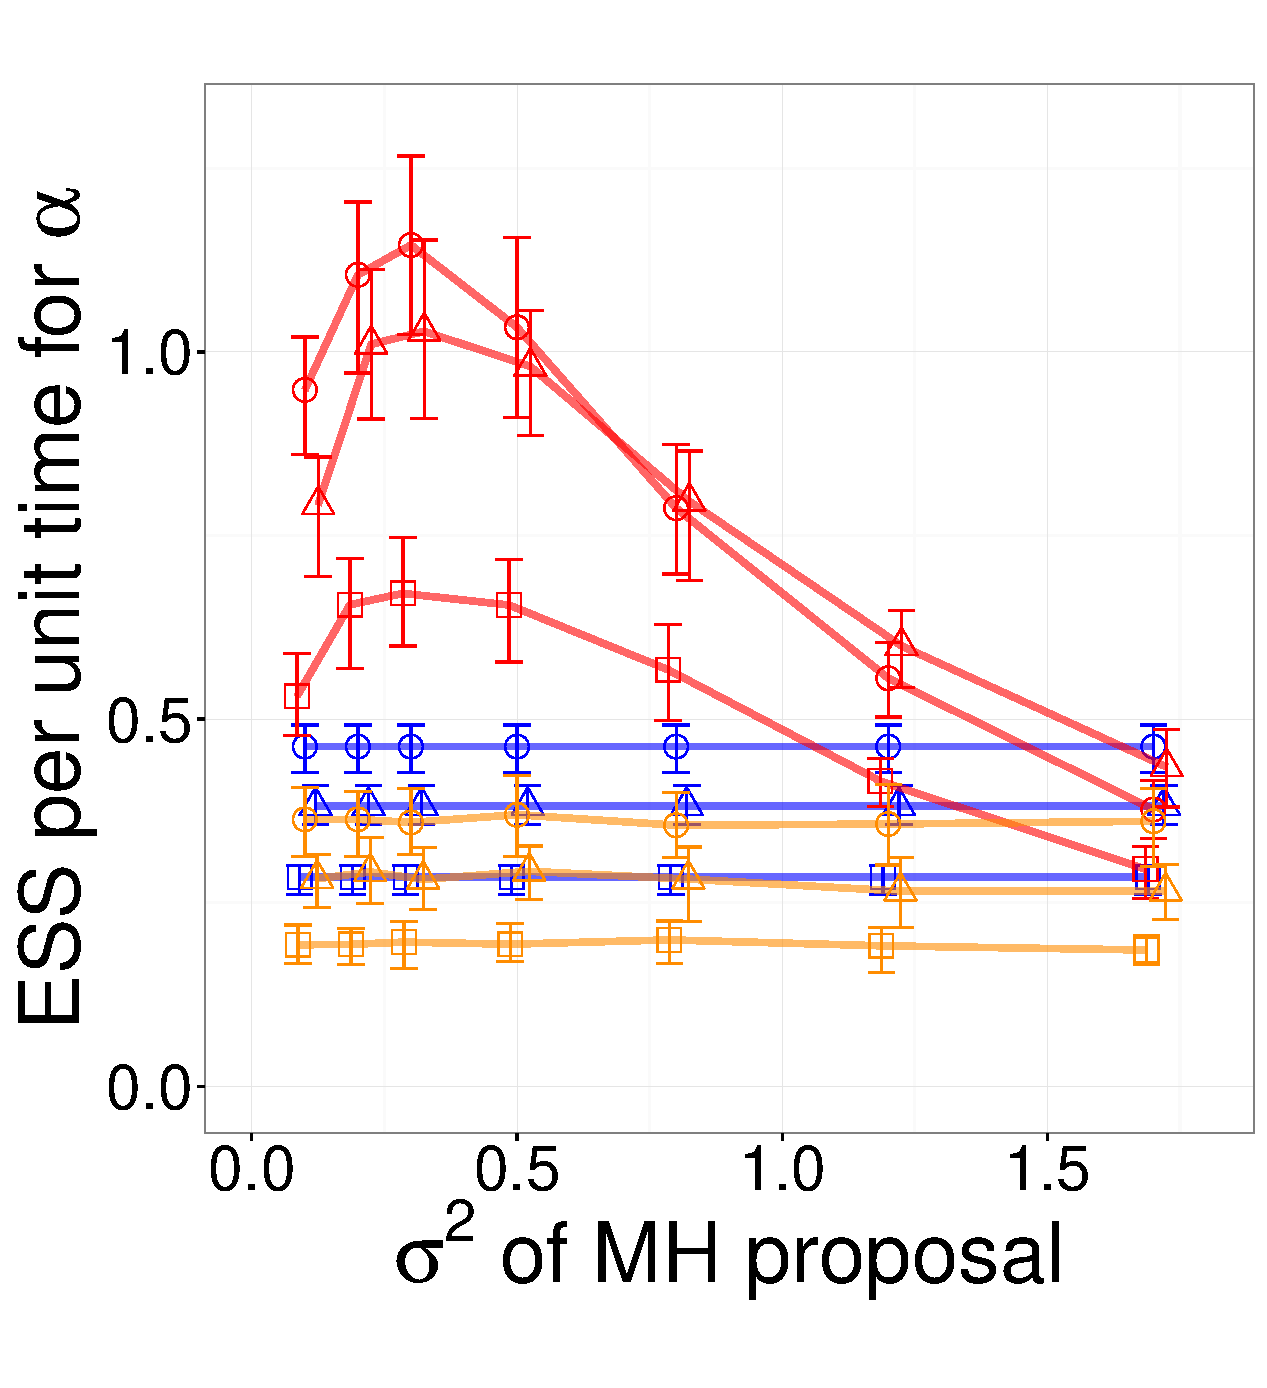
\includegraphics [width=0.70\textwidth, angle=0]{figs/pc_5_alpha.pdf}
      \end{minipage}
  \begin{minipage}[!hp]{0.45\linewidth}
  \centering
    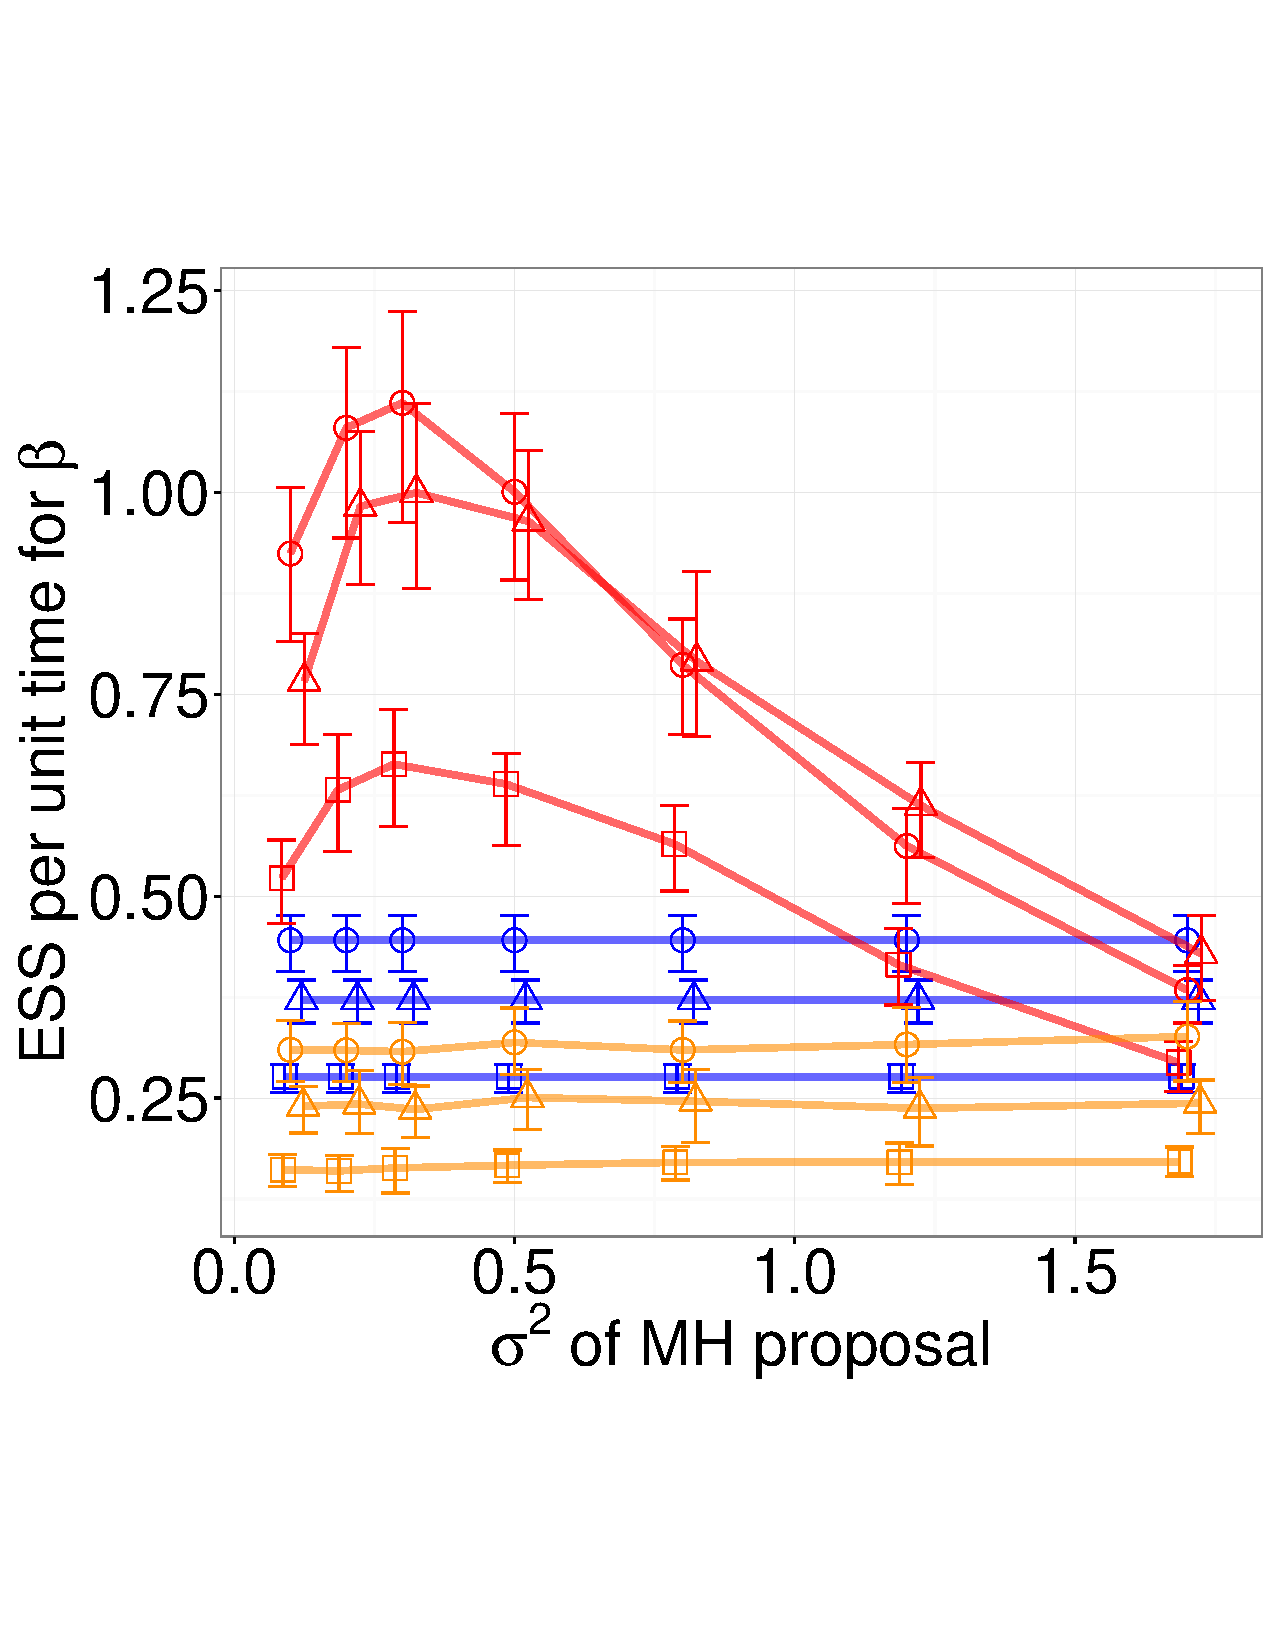
\includegraphics [width=0.70\textwidth, angle=0]{figs/pc_5_beta.pdf}
    \vspace{-0 in}
     \label{fig:ESS_Q_5}
  \end{minipage}
    \caption{ESS/sec for NH Immigration model (dim 5)}
  \end{figure}

  \begin{figure}%[b]
  \centering
  \begin{minipage}[!hp]{0.45\linewidth}
  \centering
    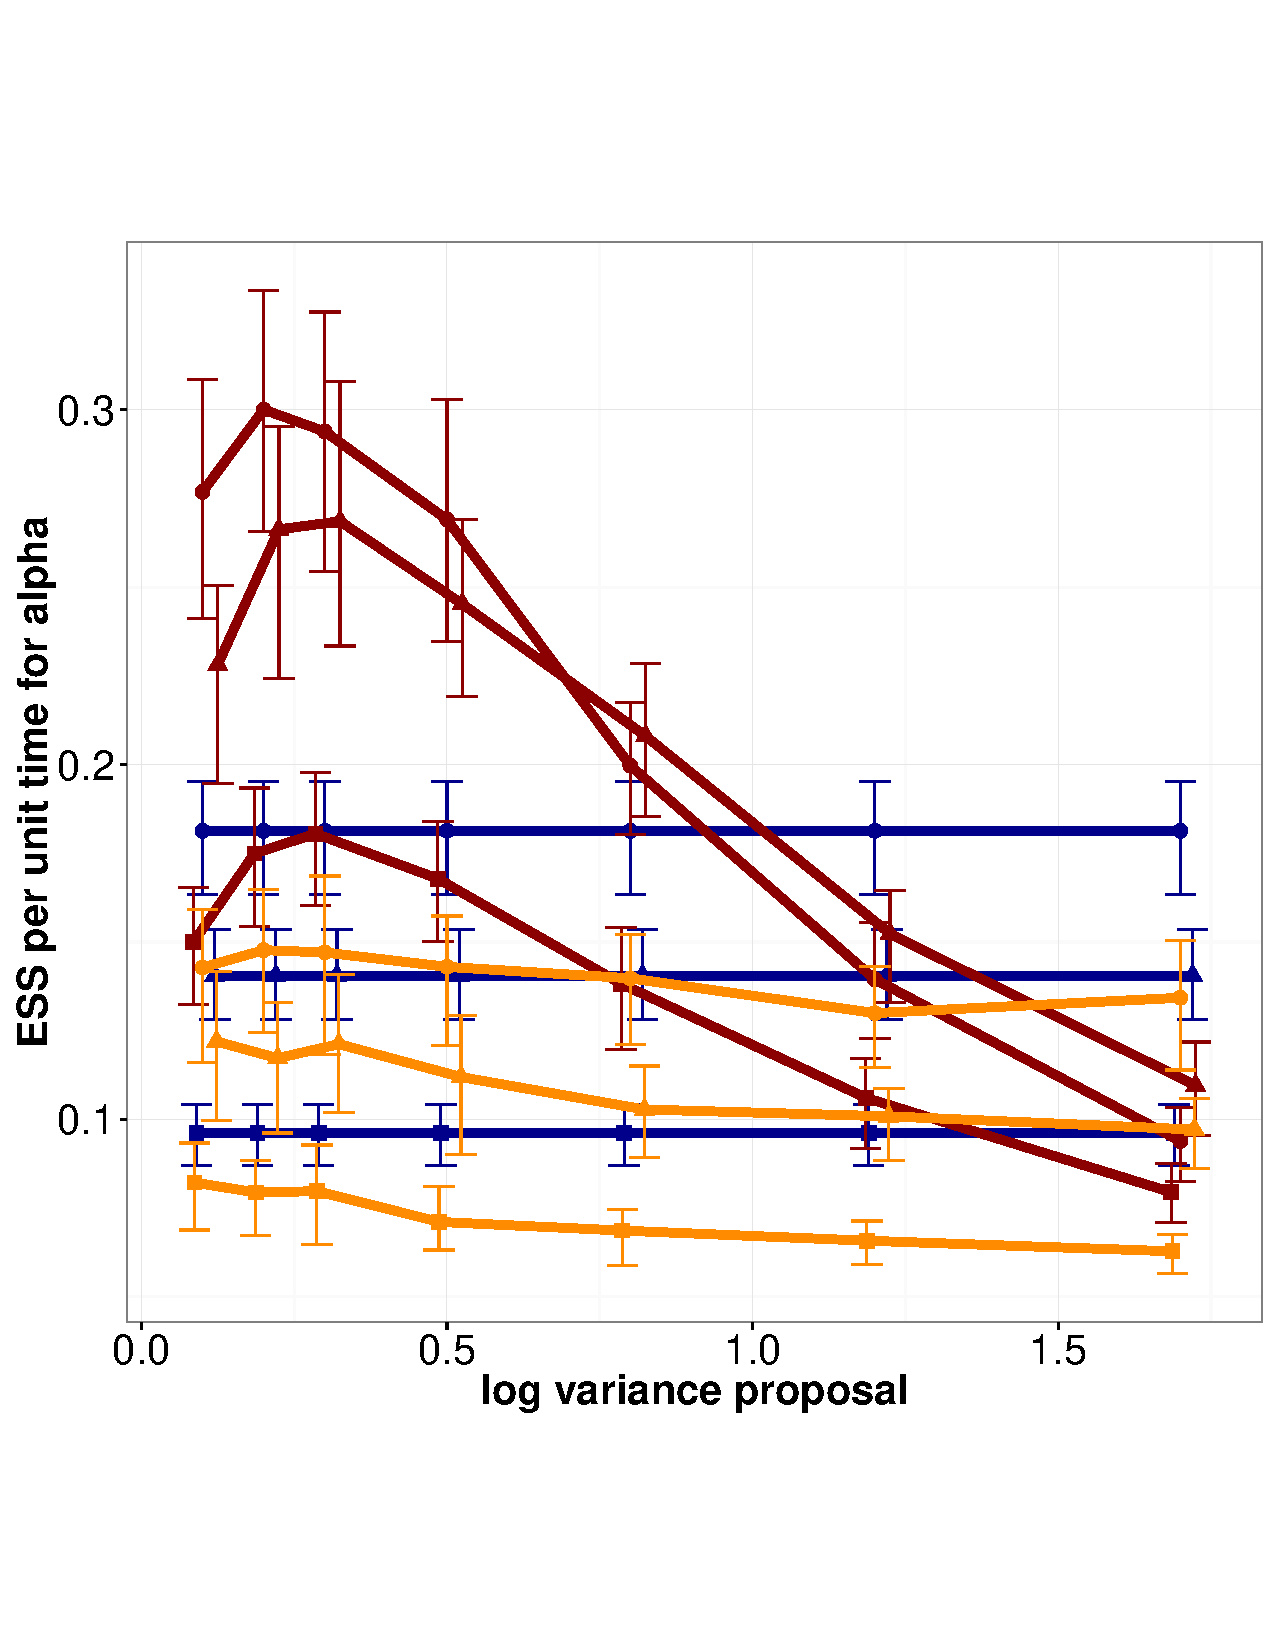
\includegraphics [width=0.70\textwidth, angle=0]{figs/pc_10_alpha.pdf}
      \end{minipage}
  \begin{minipage}[!hp]{0.45\linewidth}
  \centering
    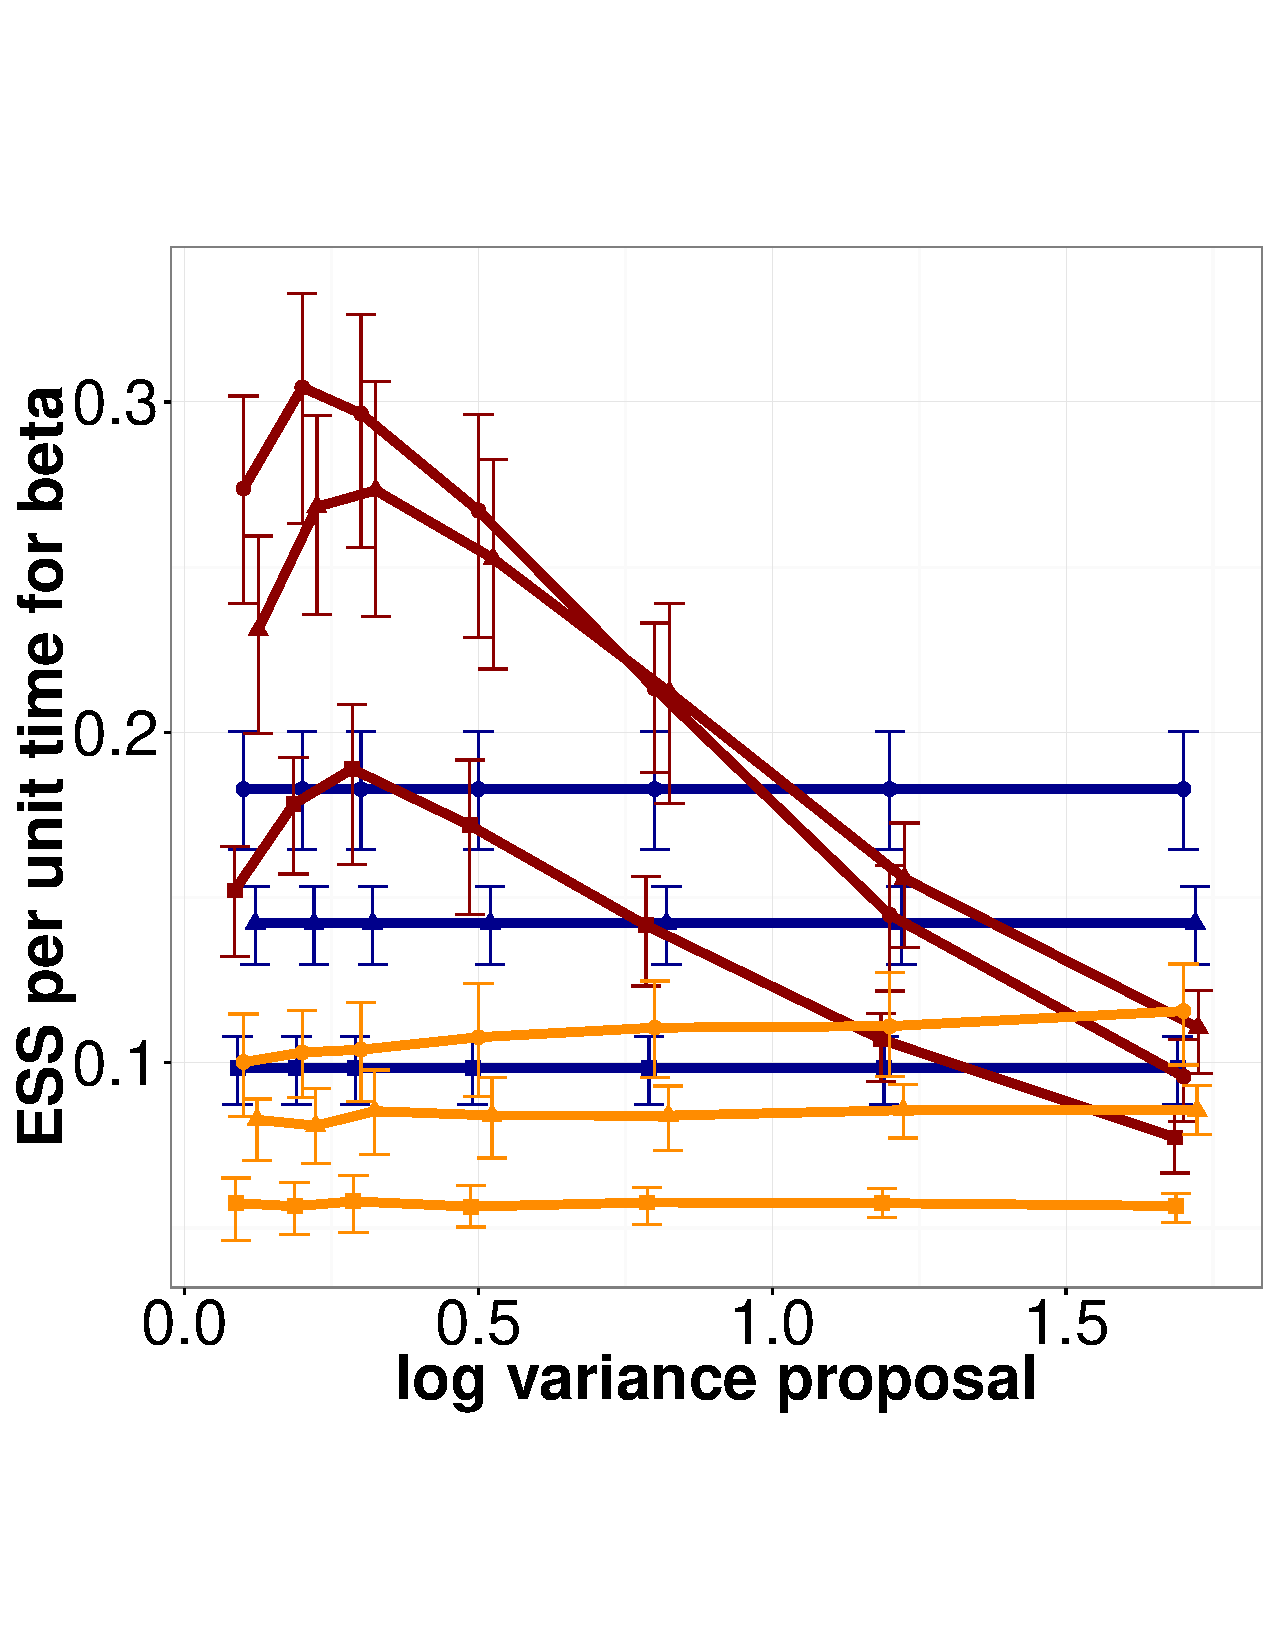
\includegraphics [width=0.70\textwidth, angle=0]{figs/pc_10_beta.pdf}
    \vspace{-0 in}
     \label{fig:ESS_Q_10}
  \end{minipage}
    \caption{ESS/sec for NH Immigration model (dim 10)}
  \end{figure}





\bigskip
%\begin{center}
%{\large\bf SUPPLEMENTAL MATERIALS}
%\end{center}

%\begin{description}

%\item[Title:] Brief description. (file type)

%\item[R-package for  MYNEW routine:] R-package �MYNEW� containing code to perform the diagnostic methods described in the article. The package also contains all datasets used as examples in the article. (GNU zipped tar file)

%\item[HIV data set:] Data set used in the illustration of MYNEW method in Section~ 3.2. (.txt file)

%\end{description}

~\cite{RaoTeh13}
~\cite{RaoTeh12}
~\cite{Andrieu10}
~\cite{Andrieu09}
~\cite{Golightly15}
~\cite{Andrieu102}
~\cite{Liu94}
~\cite{Neal12}
~\cite{Neal03}
\bibliography{bibfile}
\bibliographystyle{plain}
\end{document}
